% Options for packages loaded elsewhere
\PassOptionsToPackage{unicode=true}{hyperref}
\PassOptionsToPackage{hyphens}{url}
%
\documentclass[
]{book}
\usepackage{lmodern}
\usepackage{amssymb,amsmath}
\usepackage{ifxetex,ifluatex}
\ifnum 0\ifxetex 1\fi\ifluatex 1\fi=0 % if pdftex
  \usepackage[T1]{fontenc}
  \usepackage[utf8]{inputenc}
  \usepackage{textcomp} % provides euro and other symbols
\else % if luatex or xelatex
  \usepackage{unicode-math}
  \defaultfontfeatures{Scale=MatchLowercase}
  \defaultfontfeatures[\rmfamily]{Ligatures=TeX,Scale=1}
\fi
% Use upquote if available, for straight quotes in verbatim environments
\IfFileExists{upquote.sty}{\usepackage{upquote}}{}
\IfFileExists{microtype.sty}{% use microtype if available
  \usepackage[]{microtype}
  \UseMicrotypeSet[protrusion]{basicmath} % disable protrusion for tt fonts
}{}
\makeatletter
\@ifundefined{KOMAClassName}{% if non-KOMA class
  \IfFileExists{parskip.sty}{%
    \usepackage{parskip}
  }{% else
    \setlength{\parindent}{0pt}
    \setlength{\parskip}{6pt plus 2pt minus 1pt}}
}{% if KOMA class
  \KOMAoptions{parskip=half}}
\makeatother
\usepackage{xcolor}
\IfFileExists{xurl.sty}{\usepackage{xurl}}{} % add URL line breaks if available
\IfFileExists{bookmark.sty}{\usepackage{bookmark}}{\usepackage{hyperref}}
\hypersetup{
  pdftitle={Decision Modeling with Spreadsheets},
  pdfauthor={William G. Foote},
  hidelinks,
}
\urlstyle{same} % disable monospaced font for URLs
\usepackage{longtable,booktabs}
% Allow footnotes in longtable head/foot
\IfFileExists{footnotehyper.sty}{\usepackage{footnotehyper}}{\usepackage{footnote}}
\makesavenoteenv{longtable}
\usepackage{graphicx,grffile}
\makeatletter
\def\maxwidth{\ifdim\Gin@nat@width>\linewidth\linewidth\else\Gin@nat@width\fi}
\def\maxheight{\ifdim\Gin@nat@height>\textheight\textheight\else\Gin@nat@height\fi}
\makeatother
% Scale images if necessary, so that they will not overflow the page
% margins by default, and it is still possible to overwrite the defaults
% using explicit options in \includegraphics[width, height, ...]{}
\setkeys{Gin}{width=\maxwidth,height=\maxheight,keepaspectratio}
\setlength{\emergencystretch}{3em} % prevent overfull lines
\providecommand{\tightlist}{%
  \setlength{\itemsep}{0pt}\setlength{\parskip}{0pt}}
\setcounter{secnumdepth}{5}
% Redefines (sub)paragraphs to behave more like sections
\ifx\paragraph\undefined\else
  \let\oldparagraph\paragraph
  \renewcommand{\paragraph}[1]{\oldparagraph{#1}\mbox{}}
\fi
\ifx\subparagraph\undefined\else
  \let\oldsubparagraph\subparagraph
  \renewcommand{\subparagraph}[1]{\oldsubparagraph{#1}\mbox{}}
\fi

% Set default figure placement to htbp
\makeatletter
\def\fps@figure{htbp}
\makeatother

\usepackage{booktabs}
\usepackage[]{natbib}
\bibliographystyle{apalike}

\title{Decision Modeling with Spreadsheets}
\author{William G. Foote}
\date{2021-05-08 to 2021-05-16}

\begin{document}
\maketitle

{
\setcounter{tocdepth}{1}
\tableofcontents
}
\hypertarget{prerequisites}{%
\chapter*{Prerequisites}\label{prerequisites}}
\addcontentsline{toc}{chapter}{Prerequisites}

The material in this book arises from several years of quantitative consulting for management and executive decision makers across several industries including government entities and from teaching MBA courses at Manhattan College. The materials in this book form the content for a focused one term, 3-credit graduate core course in an MBA program. As the title indicates the primary goal is to model decisions organizations and their decision makers face. These include hiring, making, marketing, financing, procuring, distributing, developing, and strategizing what they produce and serve to customers, employees, investors, vendors, and, yes, regulators.

The primary computer software platform will be Excel 2019 with the Solver add-in. The course platform consists of the companion files from Microsoft as well as any file in Moodle. I do not recommend the use of Google Spreadsheets, yet. They often do not support some of the more basic structures of Excel, including the charting object (plots), the pivot table object, and macro recording. There is the smallest amount of programming in Visual Basic for Applications to automate the heavier computational loads of simulation. The goal, computationally, has been to use whereever possible what is native to the spreadsheet environment without use the of external calls to vast computational environments where algorithms alas are behind the proverbial curtain.

Here is a sample weekly schedule for a 7 week course.

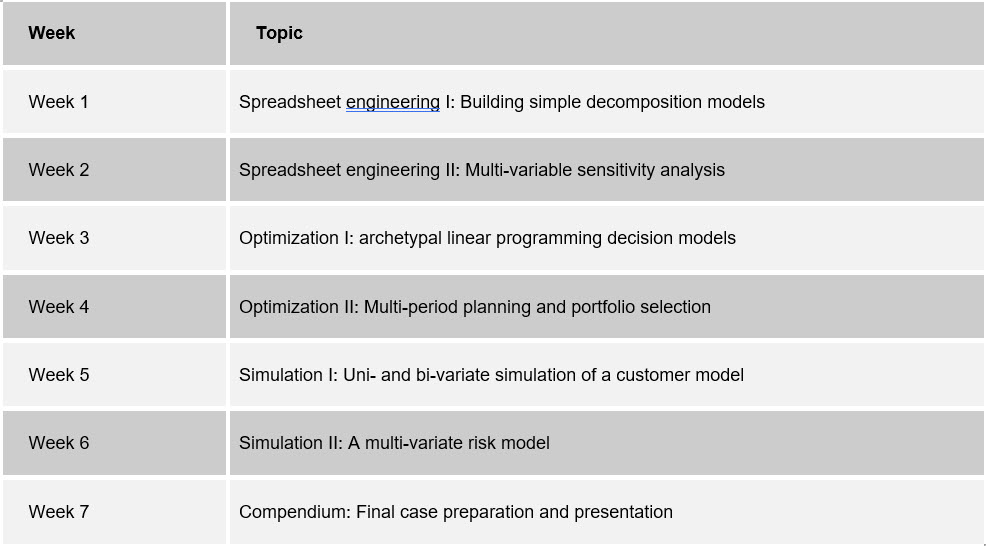
\includegraphics{images/01/weekly-schedule.jpg}

The book may be used to supplement much larger tomes devoted to the entire span of management science and computing techniques. The approach taken in this book is to titrate, curate, and focus students and practitioners on the essentials of using spreadsheets carefully in developing rapid prototype models of decisions in the field. The panoply of models that could have made the cut, but did not, underscores the need for a principled focus on essential model building and implementation in a spreadsheet.

With the essentials in hand, and in practice, analysts will have a solid basis to build prototypical models that can be expanded horizontally across other model configurations and vertically through various decision making requirements. As such, for example, network models are not discussed but are used to present the basics of a planning model. Also the range of Monte Carlo simulation is barely touched, but its utility is exploited with an uncommonly found model of a thick tail event distribution.

\hypertarget{part-1-spreadsheet-engineering}{%
\chapter*{Part 1 -- Spreadsheet Engineering}\label{part-1-spreadsheet-engineering}}
\addcontentsline{toc}{chapter}{Part 1 -- Spreadsheet Engineering}

Getting our arms around

\begin{itemize}
\item
  Design models with influence diagrams
\item
  Deploy principles of good spreadsheet practice
\item
  Use named ranges with INDIRECT, search with INDEX, MATCH, aggregate with SUMPRODUCT
\item
  Basic, non-probabilistic, sensitivity analysis with Data Table
\item
  Basic, non-probabilistic, sensitivity analysis with VBA
\item
  One variable optimization by grid approximation with Data Table
\item
  Plotting to communicate with a simple dashboard
\end{itemize}

\hypertarget{spreadsheet1}{%
\chapter{Tortuous Pie-making in the Sky}\label{spreadsheet1}}

\hypertarget{spreadsheets-really}{%
\section{Spreadsheets? Really?}\label{spreadsheets-really}}

Yes, emphatically! George Gilder says we should waste transistors (that is chips).\footnote{See \href{https://gilderpress.com/2020/03/12/investors-should-ignore-materialistic-superstitions/}{Gilder's comments here}. He goes on to a further idea: build billions of 1-chip interconnected systems (our mobile phones that are really computers) and waste chips that way instead of manufacturing billion chip data centers. According to Moore's law we will eventually get to a near zero-cost chip.} Gilder makes the fairly obvious point that we must use transistors (lots of them in an integrated circuit) or go out of business. They are ubiquitous. And arrived everywhere in a very short amount of time to boot. If you do not use them you lose control of your cost structure. Anything you build will be too expensive, too heavy, too big, too slow, too lacking in quality.

The same idea goes with Michael Schragge builds on Gilder's ironic hyperbole about transistors and analogizes that we should ``waste simulations.''\footnote{Here is a \href{https://www.technologyreview.com/2004/07/01/40161/prepared-minds-favor-chance/}{taste of Schrage's points of view}. He compiled the \href{https://www.amazon.com/exec/obidos/ASIN/0875848141/softwgardeinc}{``wasting prototyping'' paradigm into this book a couple of decades ago}.} If we do not so-called waste prototyping, rapid development, simulating potential problems, solutions, we will also go out of business. We must simulate until we drop! The alternative is that we will miss the one opportunity to improve or the one error that eliminates us. Of course the point he makes is that it iss not a waste, rather we should never shy away from working the problem, simulating the art of the possible.

So what is the value added of a prototype, which is simply a working model? It is about information, and information is a surprise, a deviation from a trend. Schragge believes that testing a hypothesis just gets us to the point of saying we seem, in probability that is, to have a trend going on here. In the world of growth, opportunity, error and ignorance, having a trend is barely the beginning of our journey. It is the deviation from the trend that matters.

Are we still talking about spreadhseets? Schragge quotes Louis Pasteur: ``Chance favors the prepared mind.'' Here the prepared mind is a product of simulations, the rapidly developed prototypes, Fleming used agar and discovered penicillin -- completely unexpected! Dan Bricklin developed the spreadsheet IBMDOS/Apple IIe program Visicalc.\footnote{\href{https://en.wikipedia.org/wiki/Dan_Bricklin}{Here is a summary of his work.} His innovation with Visicalc was to transform 20 hours of work into 15 minutes, almost of play at the time. Visicalc first ran on the Apple IIe. Dan is working on a web-based WikiCalc these days.} As a complete surprise this product was able to be used by millions of people to rapidly simulate other products and services. Steve Jobs credited Visicalc with the success of the Apple IIe and the Macintosh in 1985. IBM credited it with the success of the PC. Now people had a reason to buy the PC.

Using Visicalc we were able 40 years ago to build practical, plottable, usable option pricing models which transparently allowed us to visualize the calculations directly. Financial analysts built interactive pro forma balance sheet, income statements, and cash flow statements fed from managers' expectations, scenarios, and expert knowledge of markets. These models literally paid for themselves in days, not years. The main criterion for innovation success has always been the customer's payback, not the investors. How long did it take for the customer to recoup her investment? That's the innovation criterion. The spreadsheet is a sophisticated scratchpad some have used to be a production ready system.

But what is the most important message? A working prototype should be a sandbox where everyone is willing to get in and play. It has at least to be durable enough to get to the first slate of useful comments and suggestions for further improvement. Development continues! Rick Lamers recently open sourced his \href{https://github.com/ricklamers/gridstudio?ref=hackernoon.com}{Grid Studio spreadsheet product with deep integration with Python.}

Yes, let's play.

\hypertarget{questions-questions}{%
\section{Questions, questions}\label{questions-questions}}

Some questions come to mind as we begin.

\begin{itemize}
\item
  \textbf{What will we use the spreadsheet for?} We will rapidly prototype decision support models for business.
\item
  \textbf{What's a business?} We will use a working definition: an organization of resources to reach a common goal. Yes, there is more to it than that, but it's good enough for now.
\item
  \textbf{What's a decision, you might ask?} Again we will us a working definition for the moment: a commitment by people to deploy resources over time and space in support of a common goal. Decisions work inside of interconnected processes. They are the levers that allow, or refuse, inputs to become outputs. All very abstract, but we are on course to build out our use of a spreadsheet as a prototyping tool.
\item
  \textbf{What's a model?} Any model is a human being's abstraction from reality. We will not get into the cognitive, epistemological, ontological, or even methodological questions that might arise from this definition. Even saying a word like \textbf{sweet} is an abstraction of a perception, given experience with tasting anything, and tantalizingly informed by furtive imaginations. But one point must be made. \textbf{A model is not reality.} One more thing, \textbf{knowing is not just taking a look.} After all that's why we build models. But again a decision is the result of an affirmation, a judgment. Gosh, it gets epistemological really fast. We need to visit the Philosophy Department next and soon. Back to our geocentric way of thinking.
\end{itemize}

\hypertarget{count-the-errors-of-our-ways}{%
\section{Count the errors of our ways}\label{count-the-errors-of-our-ways}}

Spreadsheets are dangerous when in the wrong hands, with stubby fingers, bad memories, lack of structure, ramshackle governance, in short, poorly engineered. Here are some indicative \href{http://www.eusprig.org/horror-stories.htm}{\textbf{horror stories} from the European Spreadsheets Risk Interest Group}.

\begin{itemize}
\item
  \href{https://www.bbc.com/news/uk-54422505}{Covid: Test error `should never have happened':} 2020-10-05. The health secretary has said a technical glitch that saw nearly 16,000 Covid-19 cases go unreported in England ``should never have happened''. The error meant that although those who tested positive were told about their results, their close contacts were not traced. By Monday afternoon, around half of those who tested positive had yet to be asked about their close contacts. The error was the use of an old Excel format. Counts exceeded the number of rows in the spreadsheet. Labour said the missing results were ``putting lives at risk''.
\item
  \href{https://www.poconorecord.com/news/20190729/ag-state-overpaid-stroudsburg-nearly-500k}{AG: State overpaid Stroudsburg PA nearly \$500K}: 29/07/2019. The district used cumulative mileage totals rather than running calculations on a sample average for vehicles, which resulted in the district significantly over reporting total mileage data, causing the subsidy overpayments. In some cases the spreadsheet was double counting total days for some of the activity runs.
  -\href{https://www.theregister.co.uk}{Emailed spreadsheet contained private data in `hidden' columns}: 22/2/2017. A company employee mistakenly emailed a spreadsheet full of 36,000 coworkers' personal details to his spouse in November, 2016, including Social Security numbers and dates of birth, all in hidden columns.
\item
  \href{http://www.reuters.com/article/us-solarcity-lazard-idUSKCN11635K}{SolarCity adviser Lazard made mistake in Tesla deal analysis}: 2016-09-01. Lazard Ltd (LAZ.N), the investment bank that advised SolarCity Corp (SCTY.O) on its \$2.6 billion sale to Tesla Motors Inc (TSLA.O), made an error in its analysis that discounted the value of the U.S. solar energy company by \$400 million, This was the result of a computational error in certain SolarCity spreadsheets setting forth SolarCity's financial information that Lazard used in its discounted cash flow valuation analyses.
\item
  \href{http://files.shareholder.com/downloads/ONE/2261602328x0x628656/4cb574a0-0bf5-4728-9582-625e4519b5ab/Task_Force_Report.pdf}{Report identifies lack of spreadsheet controls, pressure to approve, at JP Morgan}: 18 January 2013-01-13. See pages 131-132 of the JP Morgan Task Force Report ``\ldots further errors were discovered in the Basel II.5 model, including, most significantly, an operational error in the calculation of the relative changes in hazard rates and correlation estimates. Specifically, after subtracting the old rate from the new rate, the spreadsheet divided by their sum instead of their average, as the modeler had intended. This error likely had the effect of muting volatility by a factor of two and of lowering the VaR.'' As reported in {[}``A tempest in a spreadsheet''{]} (\url{http://ftalphaville.ft.com/2013/01/17/1342082/a-tempest-in-a-spreadsheet/}?) Lisa Pollack comments that ``On a number of occasions, he asked the trader to whom he reported for additional resources to support his work on the VaR model, but he did not receive any. Also it appears that he (had to?) cut a number of corners, which resulted increased operational risk and artificially low volatility numbers \ldots{} pressure was put on the reviewers to get on with approving the model.''
\end{itemize}

Could many of thesse errors have been performed in a programming language like Visual Basic for Applications (underlies Excel spreadsheets), or R, or Python? Sure and they have. What they share in common are violations of basic software engineering design principles and practices, let alone well known and implemented risk management and governance.

Of course \href{https://dilbert.com/strip/2009-05-21}{Dilbert might calm us all down a bit.} Then again, maybe it isn't the spreadsheet after all, but \href{https://dilbert.com/strip/1995-08-13}{the strange idea about ant farms that someone might come up with in the first place.}

\hypertarget{prevailing-recommended-practices}{%
\section{Prevailing recommended practices}\label{prevailing-recommended-practices}}

We might refrain from using the term \emph{best practices} as that means, literally, there are no possibilities of improvement. At best, then, we might see some aspirational \textbf{leading practices}. here are some at least recommended practices for our consideration. They are based on this selection.

\begin{itemize}
\item
  \href{https://arxiv.org/ftp/arxiv/papers/0909/0909.2452.pdf}{Susan Allen's work at Lloyds Bank}
\item
  \href{https://arxiv.org/ftp/arxiv/papers/0803/0803.0165.pdf}{Payette's documenting spreadsheets,}
\item
  \href{https://arxiv.org/ftp/arxiv/papers/0803/0803.0165.pdf}{Various guidelines compiled by Raffensperger}
\item
  An all time favorite still \href{http://www.eusprig.org/smbp.pdf}{Read and Batson's IBM spreadsheet modeling design practices from way back in 1999.}
\end{itemize}

\hypertarget{do-not-ever-do-this}{%
\subsection{Do not ever do this}\label{do-not-ever-do-this}}

\begin{enumerate}
\def\labelenumi{\arabic{enumi}.}
\item
  Hard code data in a formula
\item
  Take the word \emph{spread} in spreadsheet literally
\item
  Put more than one major task or component on a worksheet
\item
  Guess the length or dimensions of any array, and everything in a spreadsheet is an array;
\item
  Use more than 3 IF-THEN-ELSE's nested in a single formula
\item
  Calculate parameters inside a chart or presentation table
\item
  Use Excel as the standard system of record database
\item
  Pretend you don't know what a named range is.
\end{enumerate}

\hypertarget{instead-practice-these}{%
\subsection{Instead practice these}\label{instead-practice-these}}

\begin{enumerate}
\def\labelenumi{\arabic{enumi}.}
\item
  Work flow. Paper and pencil the work flow for a model first. Document the scope, timing, user and system requirements, testing criteria first. Put data in one worksheet, task 1 in another, task 2, in another, and so on, plot set-up, table set-up in other separate worksheets, end-user presentation in another worksheet. Treat the spreadsheet model like a 3rd normal form data base. But for goodness sake avoid using Excel as a system of record data base if you can!
\item
  Definitions. Use named ranges to refer to any cell or array by name. Refer to cells and arrays where appropriate with INDIRECT(). This is what programming languages do. Each object has a unique name and scope of operations (e.g., integer, floating point, character data, class, slot) with descriptions in comments, Named ranges has some of this capability to document what the cells are and a bit of what they are meant to do. Named ranges are effectively row and column absolute addresses where cell data resides in worksheets. Attributes of cells include value, format, data type.
\item
  Testing. Be ready to test the model. Paper and pencil calculations should yield the same calculations for bits of the model, often called a \emph{unit test}. But does the whole model stand up to scrutiny? A testing plan would stretch every assumption even to the breaking point of the model. Such \emph{stress testing} and \emph{system testing} are critical to the credibility both of the model and the model-builder in the eyes of the consumer of the model's results. The resiliency of models to changes in assumptions can be tested by installing form controls to sensitize results to those changes.
\item
  There are many more good practices, and even more bad ones. We should keep working, testing, improving, and communicating with one another about our various attempts at implementation. Perhaps a step in the right direction is the extensive use of FORMULATEXT() to display formulas in cells. Documentation can lead to immediate improvements.
\end{enumerate}

\hypertarget{pie-in-the-sky}{%
\section{Pie-in-the-Sky}\label{pie-in-the-sky}}

Simone Tortiere makes pies: gluten-free, vegan, full of micro-nutrients. She targets a highly under-served niche market: nutritarians. She has a dilemma. She would like to expand her business. The problem is what price should she charge? Simple economics usually indicates the price that yields the highest profit.

Here is some data at hand Tortiere finds credible enough to use along with some questions to which she wants answers.

\begin{itemize}
\item
  \textbf{Value capture}. Make-A-Pie Co.~generates profit by combining two purchased ingredients (fruit and dough) into pies, processing the pies (cooking, packaging, \& delivering), and selling them to local grocery stores. \textbf{What are the determinants of profit?}
\item
  \textbf{Processing}. Make-A-Pie keeps track of weekly processing costs. The table below shows expense for various output levels. \textbf{What is the relationship between output volume and expense?}
\end{itemize}

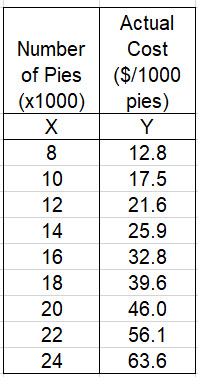
\includegraphics{images/01/pie-cost-table.jpg}

\begin{itemize}
\item
  \textbf{Demand}. Make-A-Pie has also experimented with demand elasticity. At a price above \$12, there will be no demand for her pies, but demand increases by about 4,000 pies per week for each dollar price decrease below \$12. For example, at a price of \$10 Make-A-Pie could expect demand of 8,000 pies. \textbf{What is the average relationship between price and revenue?}
\item
  \textbf{Price}. Savory vegetable filling costs \$3.48/pie, and sprouted flour dough costs \$0.30/pie. Overhead expenses are \$12,000 per week. \textbf{At what pie price will Make-A-Pie maximize profit? At what price will Make-A-Pie break even?}
\item
  \textbf{Sensitivity}. Tortiere believes in her estimates, but she well knows that markets, property tax assesssments, customer sentiment, and supplier costs can change. \textbf{How sensitive is weekly profit when any of the drivers of cost and revenue change?}
\end{itemize}

Tortiere muses further. She needs to understand if her business is profitable over the next few years and at what very sticky price should she charge her customers. She has already invested \$2.5 million.

\begin{itemize}
\tightlist
\item
  \textbf{Multi-period value}. Suppose that savory vegetable filling cost rises by 7\% per year, and sprouted dough rises (pun included) by 5\%. Overhead expenses rise by 2\% per year. Prices will also rise by 2\% per year. \textbf{At what year 1 pie price will Make-A-Pie maximize profit across a 3 year horizon if the business is worth \$2,500,000 today?}
\end{itemize}

Tortiere hires us to help her with her analysis. She asks us what is the first thing we should do?

\hypertarget{wheres-the-paper-and-pencils}{%
\section{Where's the paper and pencils?}\label{wheres-the-paper-and-pencils}}

First and foremost we map the requested analysis. We use a decompositional technique called an \href{http://www.cs.ru.nl/~marinav/Teaching/BDMinAI/influencediagrams05.pdf}{influence diagram, as developed by Howard and Matheson.} The diagram extends the ideas behind a similar structure called a decision tree, both of which are examples of \href{https://en.wikipedia.org/wiki/Directed_acyclic_graph}{directed acyclic graphs} and \href{https://escholarship.org/uc/item/6gv9n38c}{causal inference, e.g., Judaea Pearl's work} Software such as \href{http://www.dagitty.net/}{dagitty} can greatly aid visualization of causal relationships among decisions (e.g., price), criteria (e.g., profit), and drivers (e.g., unit costs). After all of that consideration here we will simply use boxes and arrows.

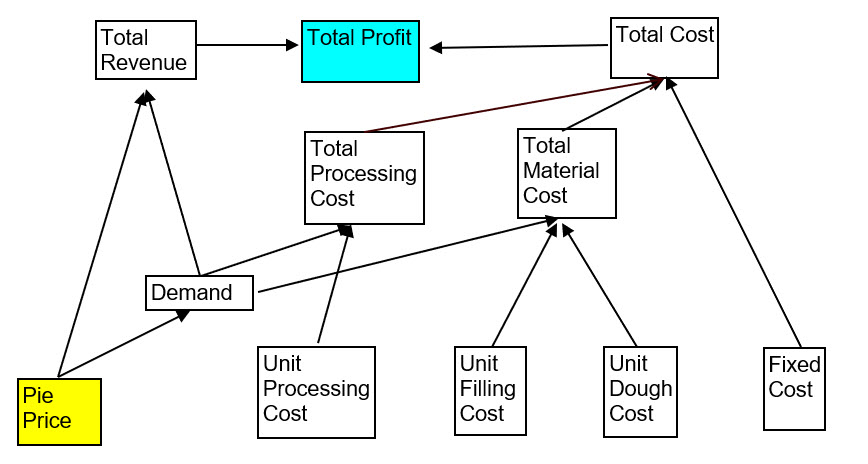
\includegraphics{images/01/pie-influence-diagram.jpg}

We identify the decision as price in the yellow box and the decision criterion profit in the blue box. Price, unit and fixed costs are somehow exogenous since they do not depend on any variable, but they do determine other variables. Unit and fixed costs will be assumed and thus condition the rest of the variables. Price on the other hand is the one variable for which we solve. Literally we will pick a price and see what happens to profit.

Tortiere agrees with our approach and analysis. She sees that her efforts to understand how the demanded volume of pies sold depends on her pricing decision. But she wants to get at how volume influences, conditions, cost. We move to the next task, the cost structure.

\hypertarget{cost-and-volume}{%
\section{Cost and volume}\label{cost-and-volume}}

Make-a-Pie's experience with expense and volume provides some inside into the way volume, as determined by number of pies sold, will influence, condition, cost. Here is a scatter plot with linear and quadratic lines fit to the data.\footnote{See \citet{Winston2019}, Chapter 54 Charting Tricks is a one-stop destination for a variety of charts, including the scatter plot here.}

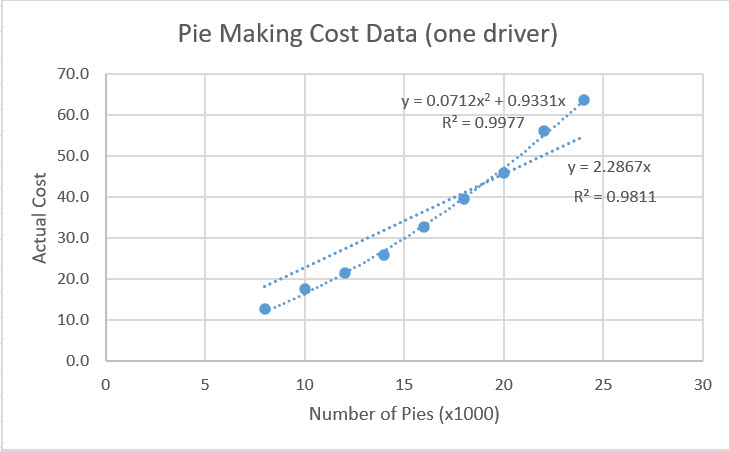
\includegraphics{images/01/pie-xost-graph.jpg}

Right-clicking one of the blue observations will reveal a dialogue box with a Trendline feature. This produced the lines and the equations. We can check these results by hand, but let's use the LINEST array function instead in the cost worksheet.\footnote{\citet{Winston2019} discusses several array functions and formulas in Chapter 91 and LINEST at page 578. LINEST is \href{http://www.mit.edu/~mbarker/formula1/f1help/04-g-m60.htm}{discussed here as well} along with references to array functions. To enter an array function: 1. Select a results range. Some functions require the results range to contain a certain number of columns or rows. A an abridged results range will not show all of the function results; a results range that is longer than the function's capability will display error messages in some cells. Check the documentation on the specific function for information about the required size and shape of the results range. 2. In the results range you selected, type in the equals sign, the array function keyword, and the argument(s) or argument range(s), in parentheses. 3. To enter the function DO NOT PRESS ENTER! Instead press SHIFT and CONTROL together and while they are pressed down then press ENTER. (If you simply press ENTER, the array function will return the \#VALUE! error.)}

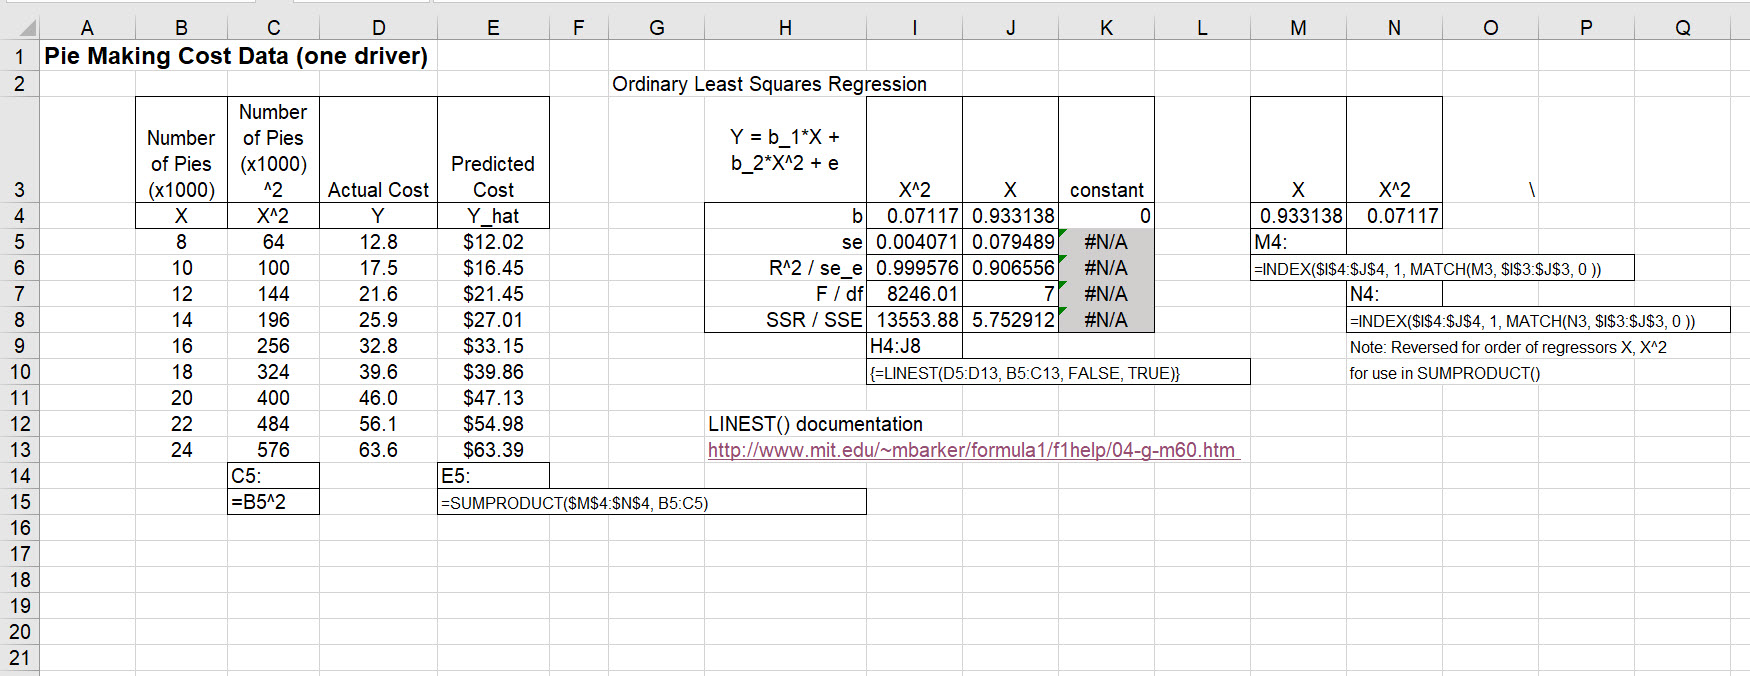
\includegraphics{images/01/pie-cost.jpg}
The FALSE setting in LINEST sets the intercept to zero in the Ordinary Least Squares (OLS) estimation. Predicted costs will be used in the profit calculation using volume demanded as an input to the quadratic cost structure. We also use the INDEX-MATCH combination to wrangle coefficients for use in the SUMPRODUCT calculation.\footnote{See \citet{Winston2019} Chapters 4 and 5 for INDEX-MATCH and Chapter 59 for multiple regression.}

\hypertarget{demand-analysis}{%
\section{Demand analysis}\label{demand-analysis}}

Tortiere's experiments with pricing provide valuable windows into customer preferences. Even a simple change of price can reveal a conjecture about the range of preferences. In this situation we need to anchor the demand analysis around two important points:

\begin{itemize}
\item
  the give-away price and volume, and
\item
  the no-show price where volume is just zero.
\end{itemize}

The give-away price is zero at least. The volume associated this lowest price becomes the intercept of a down-ward sloping straight-line demand curve in price. The increment downward is estimated using a simple rise-over-run rate of change of volume with respect to price.

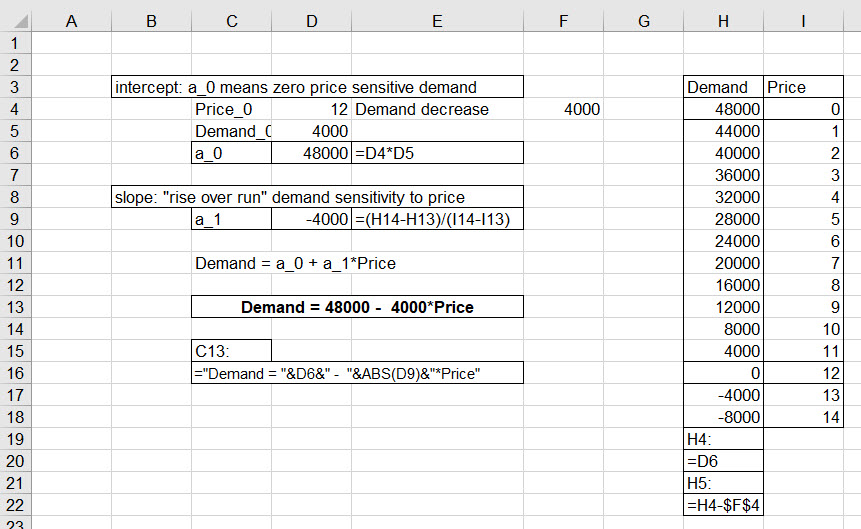
\includegraphics{images/01/pie-demand-analysis.jpg}

At a price above \$12, there will be no demand for her pies, but demand increases by about 4,000 pies per week for each dollar price decrease below \$12. For example, at a price of \$10 Make-A-Pie could expect a demand of 8,000 pies in a week. The intercept is then \(12 \times 4000 = 48000\). The formula in D9 confirms the negative slope \(-4000\). Thus we have a demand equation which serves as a schedule that will feed both revenue and processing cost.\footnote{\citet{Winston2019} Chapters 87 and 89 provide further approaches to demand analysis.}

\hypertarget{weekly-profit}{%
\section{Weekly profit}\label{weekly-profit}}

Weekly profit is only a snapshot of performance. It is defined as total revenues minus total costs with various drivers defined mapped in the influence diagram. The calculations depend on assumptions provided by another worksheet, the finale of the model, the dashboard. Cost and demand volumes derive from estimated algebraic relationships we already peaked at.

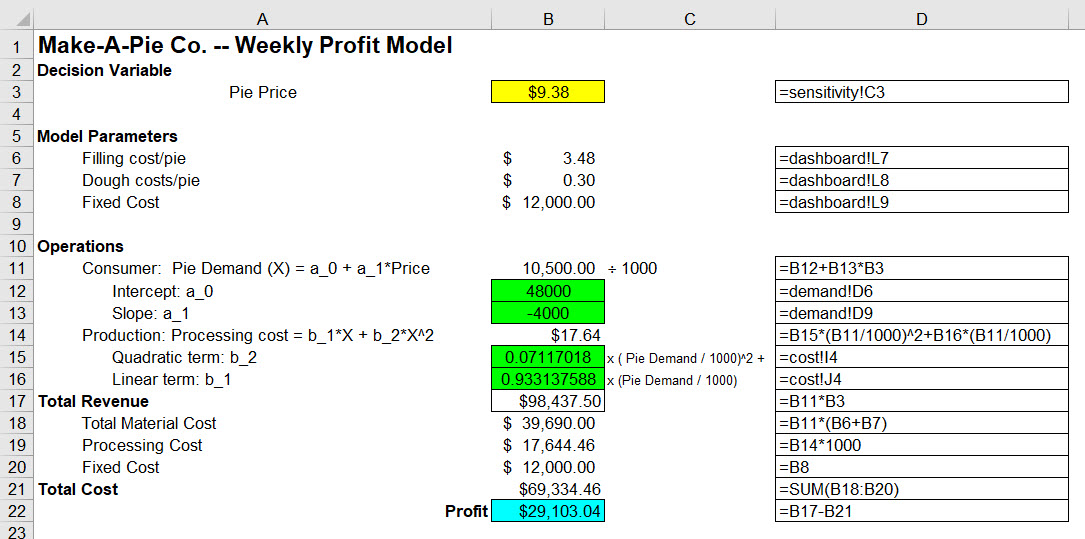
\includegraphics{images/01/pie-profit.jpg}

Price comes from a sensitivity analysis we have yet to review and is an input from that analysis of the profit maximizing price. Three unit and fixed cost assumptions also wander in from the dashboard. The user moves slide bars to choose those levels.

\hypertarget{profit-sensitivity-to-price}{%
\section{Profit sensitivity to price}\label{profit-sensitivity-to-price}}

Perhaps the most important activity in the building of a model, and the reason for a model in the first place, is to understand how model elements are sensitive to one another. Not emotionally of course as our models are robots and golems. BUt really there is no one so-called right answer! It is a range of answers dependent on the instructions we gave to our spreadsheet robots. Yes, the decision maker has to sign the contract, write a cheque, hire (or fire) a designated vendor, employee, partner. But before these decisions are cast in stone, we owe it to ourselves to waste simulations, again to recall George Gilder and Michael Schrage's ironic hyperbole.

In this graph we use data tables (Data \textgreater{} What if \textgreater{} Data Table) to take the column of possible prices and run them against the profit model. For each price (yes this is a for loop) the data table calculates a new profit.\footnote{\citet{Winston2019} Chapter 17 deftly covers this vast topic. I do not like to use data tables too extensively and without further some thought. They are dynamic. Whenever you change a cell, the table recalculates. That's fine for as simple data table as we have here. The problem is when we have a 10000 by 100 table. It simply take a while to update. The easiest way to change the calculation mode is on Excel's Formula ribbon. In the Calculation grouping, on the right side of the ribbon, is a drop-down button for \textbf{Calculation Options}. We choose an option that works best for the current file. There are two other important buttons in the Calculation grouping. \textbf{Calculate Now} (equivalent to pressing function key F9) updates the entire workbook. \textbf{Calculate Worksheet} updates only the current sheet, which is much faster in a large file.}

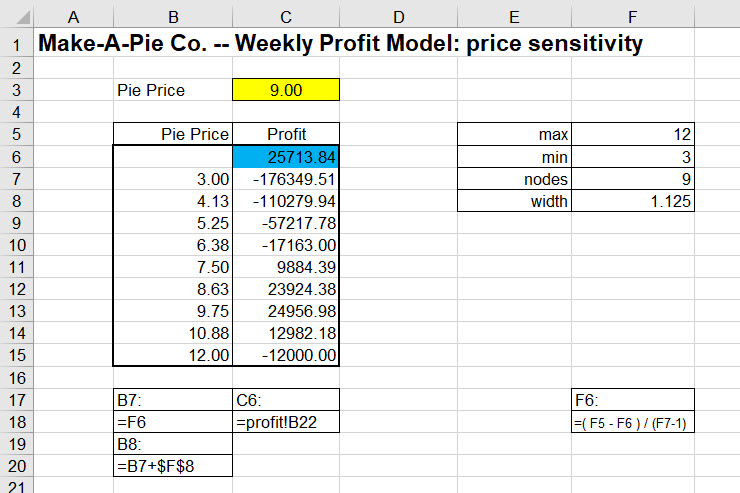
\includegraphics{images/01/pie-sensitivity-price.jpg}

A plot of price and profit is more than a little instructive. Here is a setup worksheet with titles, additional calculations and lookups. Shown only is the sensitivity table setup. Any other plots in this workbook have a setup grid devoted to their charts.

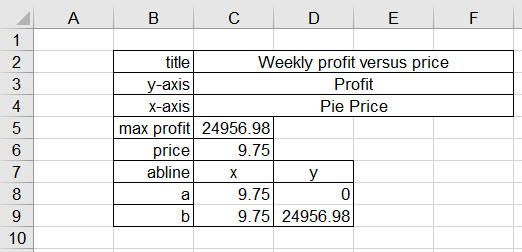
\includegraphics{images/01/pie-plot-setup.jpg}

\hypertarget{lo-and-behold}{%
\section{Lo and behold}\label{lo-and-behold}}

This is what we have been waiting for. We must first notice the modular nature of this spreadsheet application. The dashboard worksheet interacts with all but the questions worksheet, at least in this iteration of the application. All Simone Tortiere needs to do, after paying our invoice, is to put the cursor on the slide bars that help her understand how the profit maximizing price changes with changes in the unit and fixed cost assumptions.\footnote{\citet{Winston2019} Chapter 27 has a discussion on the implementation of user form controls. These are located on the Developer ribbon at the Insert button. \href{https://support.microsoft.com/en-us/topic/show-the-developer-tab-e1192344-5e56-4d45-931b-e5fd9bea2d45}{Here are directions to show this ribbon in your workbook.}}

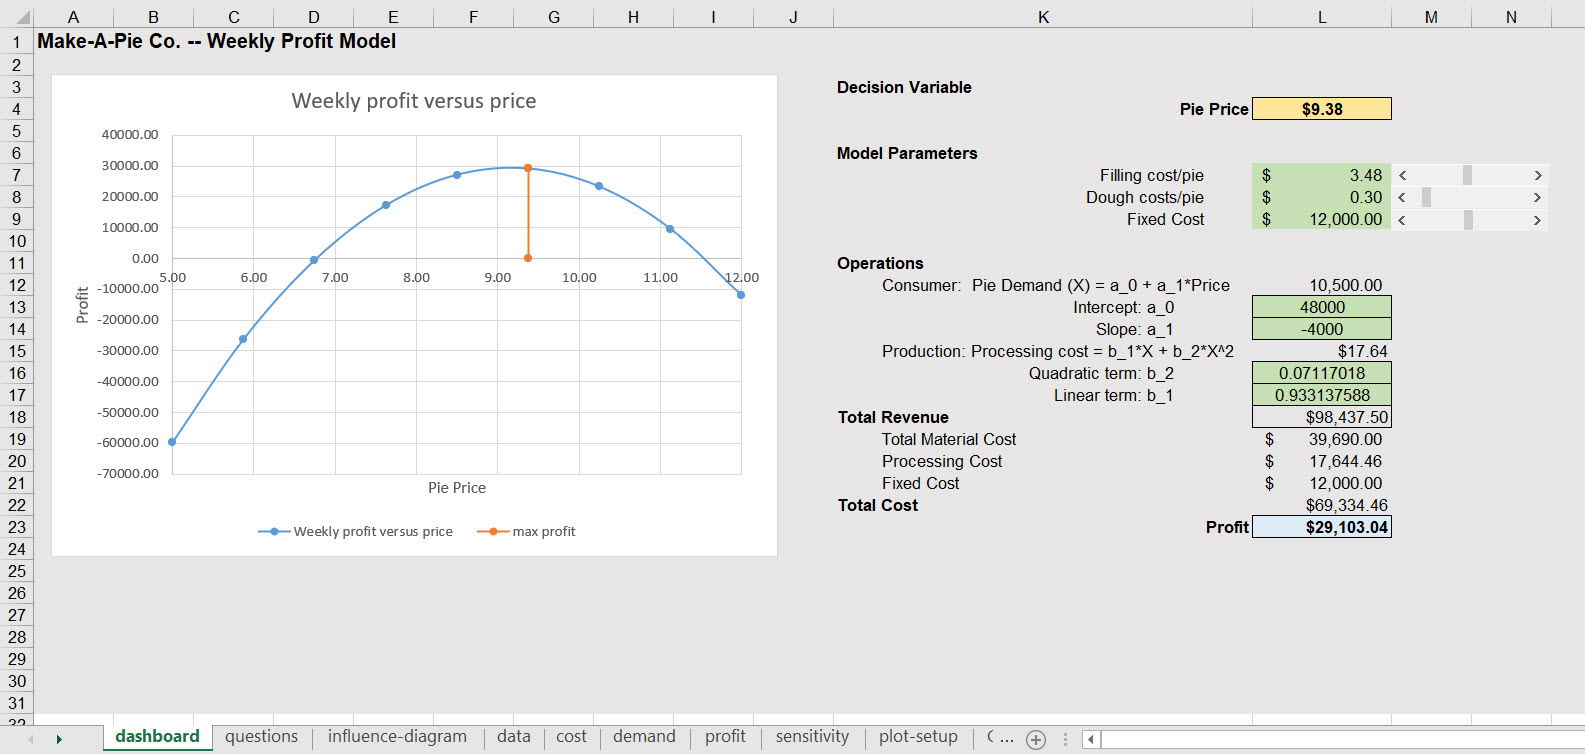
\includegraphics{images/01/pie-dashboard.jpg}

Is there too much in this dashboard? Perhaps the cost and demand equationscould be left to their respective worksheets. We might replace those with the underlying assumptions of both structures. We leave that for another day and week.

What price is best? All we have to do is live with whatever assummptions we make and read the dashboard.

\hypertarget{references-and-endnotes}{%
\section{References and endnotes}\label{references-and-endnotes}}

\hypertarget{chaotic-pie-making-in-the-sky}{%
\chapter{Chaotic Pie-making in the Sky"}\label{chaotic-pie-making-in-the-sky}}

\hypertarget{how-many}{%
\section{How many?}\label{how-many}}

According to the \href{https://irishtechnews.ie/seven-reasons-why-excel-is-still-used-by-half-a-billion-people-worldwide/?__cf_chl_jschl_tk__=eae1fe306ae27d3c9013b3704732878b80fc40f3-1616828018-0-AT1moxdZF6mKZLmtRhwzMYiVaKyU0bEe2Kz5ftdXTKKKtNdWjF6EH2e2blKxl4oVSpuFZbzH-mNHukGtzFU29btUpDwqUKJvi9xyIjQO2DmcXQ5OgccXl-AuKvdAhk9DltuuYjjrNzeh4fVzX8UvaT5nwAEAgONZ3H3GSh31P4tILL2x5OQsLXC2YFwcpthCsLENuLjGg0zZErvhaeOTbXpwVuKHBHPkZV5sZEq0wRZS6dIlxtzhO-g07UukzOtBi6GlAF_ctySgFuZ0yOwH7cFr8CzWiAUsP_GHqca5nOzJ-rbPuRMi9oc60Cb7cs7XlwM5cpxrwszbftEeCzYOV3QYkxFFKt8coSEzj5fetcnep_Fh7kEyR7xtuS5cXK_mZs8f8OkanlEyk7HesLVi0KxvIEmxk4XG1qZz8gH0DFdXYhQ2oFcLXdh4G-8gKYcwaDuvC4Ykkn2ybSU-sfazfgMLzKKIzAYgw-4r_gYvo2XG}{Irish Technology Review and quoting Microsoft} over 750 million users enjoy (?) Excel. I am enamored of points 3 and 4. I first ran into Excel with \href{}{Martha Grabowski at LeMoyne College} in 1989. I \emph{enjoyed} Lotus 1-2-3, used Visicalc, and Supercalc since 1981. I was not yet convinced about Excel. I learned C by building a very stripped down version of Borland's Quattro Pro with the idea of building option pricing models from finance directly into the DNA of the spreadsheet. We already knew that spreadsheets would inhabit if not infect the earth. My first balk was the use of the Excel \emph{=} instead of the \(@\) of Lotus formulae. Easy to overcome, but still the \(@\) (shift-2) is in my fingers' muscle memory.

I say all of this because we will see many changes in the expression of technology over the life cycle called our careers. Prepare Ye For The Changes To Come! I have experienced a lot of software products (not an expert at all and mostly a dilittante!) from very simple machine language to assembler to FORTRAN (with IMSL, LINPACK, EISPACK) to APL, APL2 (data shaping on steroids!), PLI and SAS, very early stage Matlab on DOS, S, S-Plus, LISP, PROLOG, BASIC, VBA (skipped Visual Basic interface with Oracle!), JavaScript (also skipped Java), C, C++, now R, Python, and, my almost favorite, Julia. Anything that works! Among all of these, spreadsheet products seem to have passed muster and kept going strong for the past 4 decades.

I must mention separately, \href{https://www.efinancialcareers.co.uk/news/2019/11/shakti-arthur-whitney}{Arthur Whitney's kx, A+ and Shakti} as the RISC (reduce instruction set computing) version, and maximizing time series vectors with relational databases and SQL (think vectoring FORTRAN). This is in the avant-garde of analytics. What a list of developments over the past several decades that lead us to the mixmaster and symbiosis of technology, technique, and skills we call analytics.

\href{https://www.ibm.com/products/apl2}{APL2} taught me data shaping. Whatever heuristics and algorithms within algorithms we devise in Excel are completely influenced by the shaping capabilities of array-driven technology like APL2, whether overtly or covertly. Unfortunately for a mathematically and numerically challenged population of analysts, APL2 is about to be deprecated. Yes a historically interesting, but practical issue exists? And yes, again, it does. we will develop analytically-based and at least influenced career paths that are really modeling with data paths. Musa Jafar keeps saying that there is a a 10-15 year cycle of software hegemony. I agree. The issue for us analysts is to develop capacities, not just skills in specific environments, which are agnostic to software platforms. In computing jargon, our minds must be interoperable across the platforms that enable us to inject data and interpretable analysis into our analytical products for consumption by decision makers.

Enough for this bully pulpit! The key take-away, so to say, is that we must begin with mind, go to data, and end up with mind. The mind has the thinking faculties that dicate what data is or is not important, credible, useful to the mind's view of the next horizon, whatever the technological platform.

\hypertarget{whats-new}{%
\section{What's new?}\label{whats-new}}

Simone Tortiere liked the model but furrowed her brow. Supply costs are sky-rocketing and customer demand is flagging. She is thinking about refinancing, perhaps even selling the business to a company with more capital resources. In fact she is in contact with a ;Special Purpose Acquisition Company (SPAC).{]}(\url{https://www.investopedia.com/terms/s/spac.asp}) Top of mind for her is three year plan. But first she wants to traverse the demand and cost terrain she might face. At risk is her \$2.5 million investment. She asks us to help her to revisit the pricing decision in this context.

\hypertarget{the-costs-they-are-a-changing}{%
\subsection{The costs they are a-changing}\label{the-costs-they-are-a-changing}}

Make-A-Pie is experiencing much more volatile changes in its processing costs. These represent everything from capital (think ovens) to labor (think bakers) and supporting infrastructure (think fixed costs here though). Here is a revised schedule of processing cost against volumes in thousands of pies produced in an average (actually a median) week.

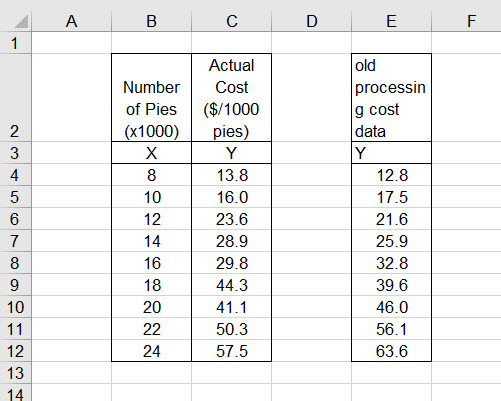
\includegraphics{images/02/pie-data-cost.jpg}

The previous schedule appears for comparison purposes. All of this calls for a new estimation of the way cost varies with pies demanded, and sold. So far storage is not an issue, yet.

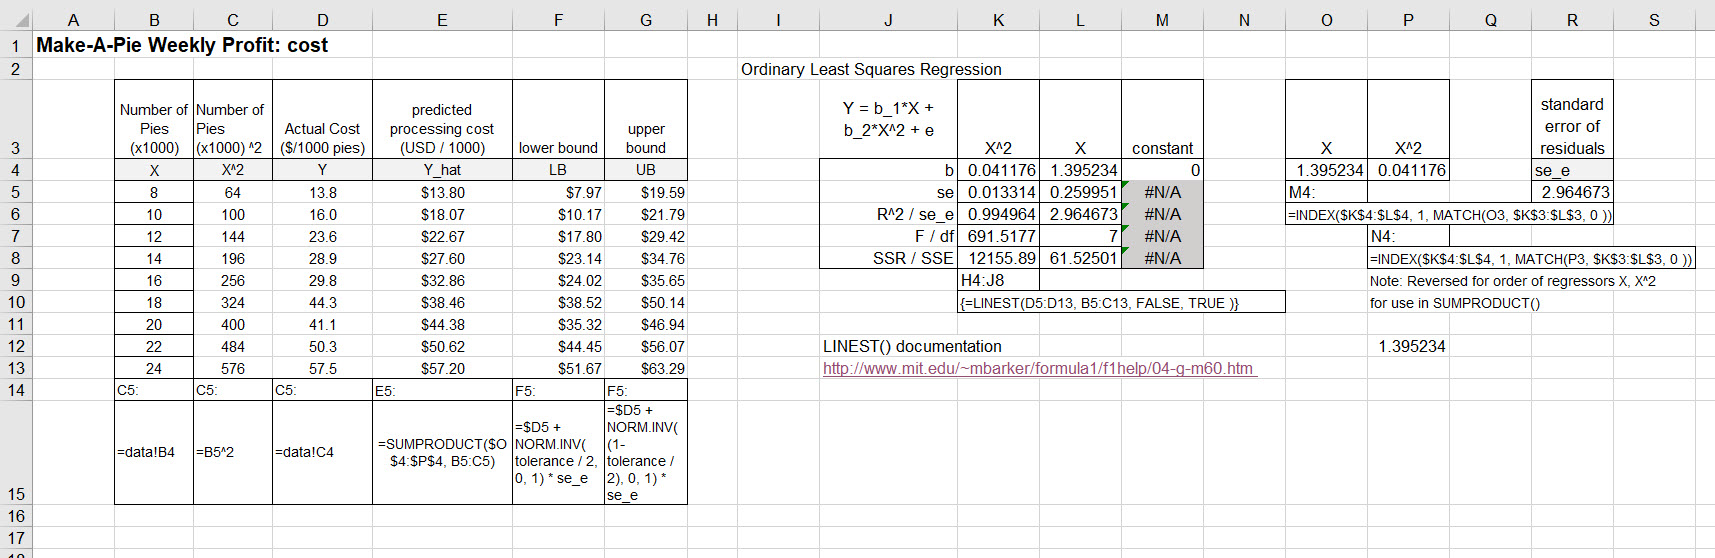
\includegraphics{images/02/pie-cost-estimation.jpg}

There is a new kid in this block of numbers. Columns F and G calculate lower \(L\) and upper \(U\) 95\% probability interval bounds. Make-a-Pie's policy is not to tolerate any more than 5\% errors in any given week. This rendering helps to explain the policy.

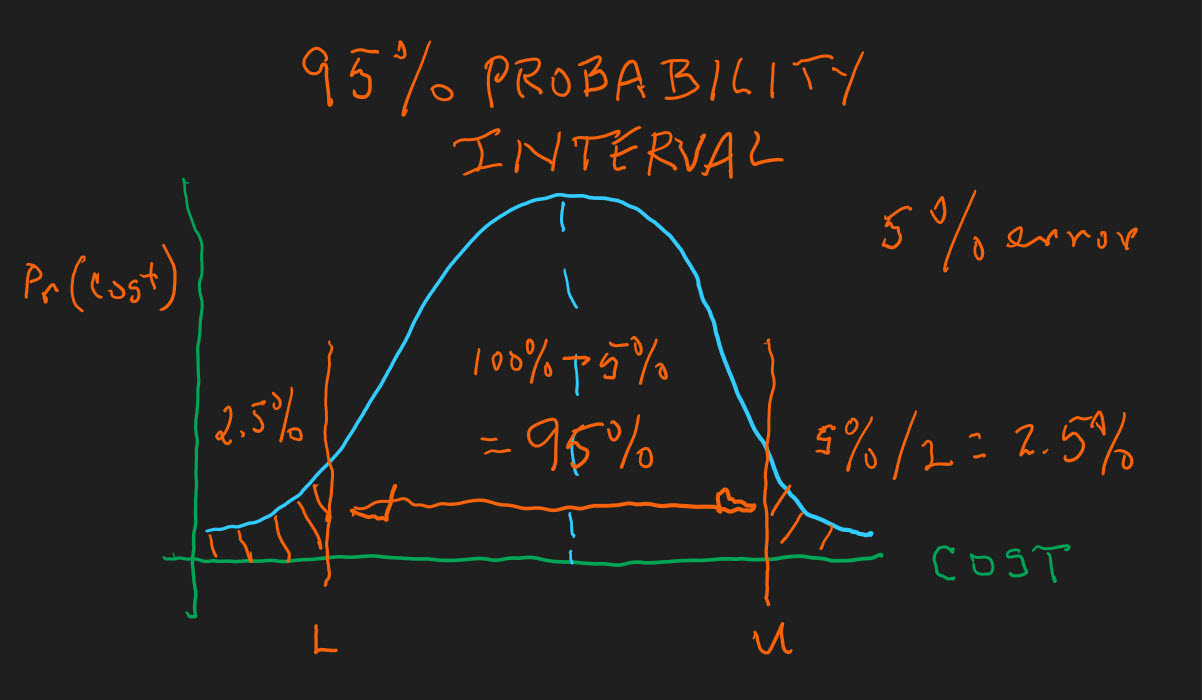
\includegraphics{images/02/pie-cost-prob-interval.jpg}

We might observe costs distributed symmetrically about a proposed future, or even actual, value. If the distribution is Gaussian, also known as normal (though there is nothing that normal about it!), then we can use Excel to calculate the lower and upper bounds of cost using the number of standard deviations \(z\) from the model mean of costs we estimated and the standard error of the model \(s_e\).

\[
\begin{align}
L &= \mu - |z_{0.025}|s_e \\
U &= \mu + |z_{0.975}|s_e
\end{align}
\]

For some mean \(\mu\) and standard deviation \(\sigma\) of observed outcomes \(X\) we can first first find the deviations of the outcome from the mean, \(X-\mu\). Then we can calculate the number of deviations per standard deviation \(\sigma\).

\[
z = \frac{X-\mu}{\sigma}
\]

We use Excel's NORM.INV() to calculate the \(z\) values with a mean of 0 and standard deviation of 1 at lower bound 2,5\% cumulative probability and upper bound 97.5\% cumulative probability. This produces the 97.5 - 2.5 = 95\% probability interval. All \(z\) distributions have this standard mean and standard deviation. That is very convenient.\footnote{\citet{Winston2019} Chapter 69 is a good and very basic introduction to random variables and Chapter 72 is a decent brief on the normal (Gaussian) distribution and z scores. We might skip ahead to Chapter 74 where he discusses the use of probability in making forecasting statements.}

Of course some errors, we might call them, are intolerable, such as breaches of legal requirements and non-compliance with regulations such as food handling. The bounds are calculated around each actual, as opposed to predicted, processing costs. A picture is much in order.

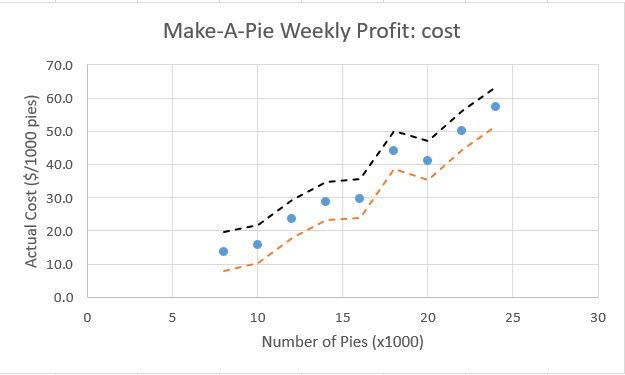
\includegraphics{images/02/pie-cost-plot-lb-ub.jpg}

There is a wide enough variation to cause further identification and assessment of root causes and potential failure modes in the operation.

\hypertarget{demand-takes-a-step-back}{%
\subsection{Demand takes a step back}\label{demand-takes-a-step-back}}

Make-a\_Pie customers buy the pies from grocery stores. Tortiere plans to set up a program with restaurants and schools as well. But we will wait for that later. Suffice it to say, such a plan will garner increased regulatory scrutiny anda requirements, all the more so-called overhead.

Recent store surveys reveal that there will be no demand for prices above \$10, but demand increases by about 4,500 pies per week for each dollar price decrease below \$10. For example, at a price of \$8 Make-A-Pie could expect demand of 9,000 pies. Here are the calculations.

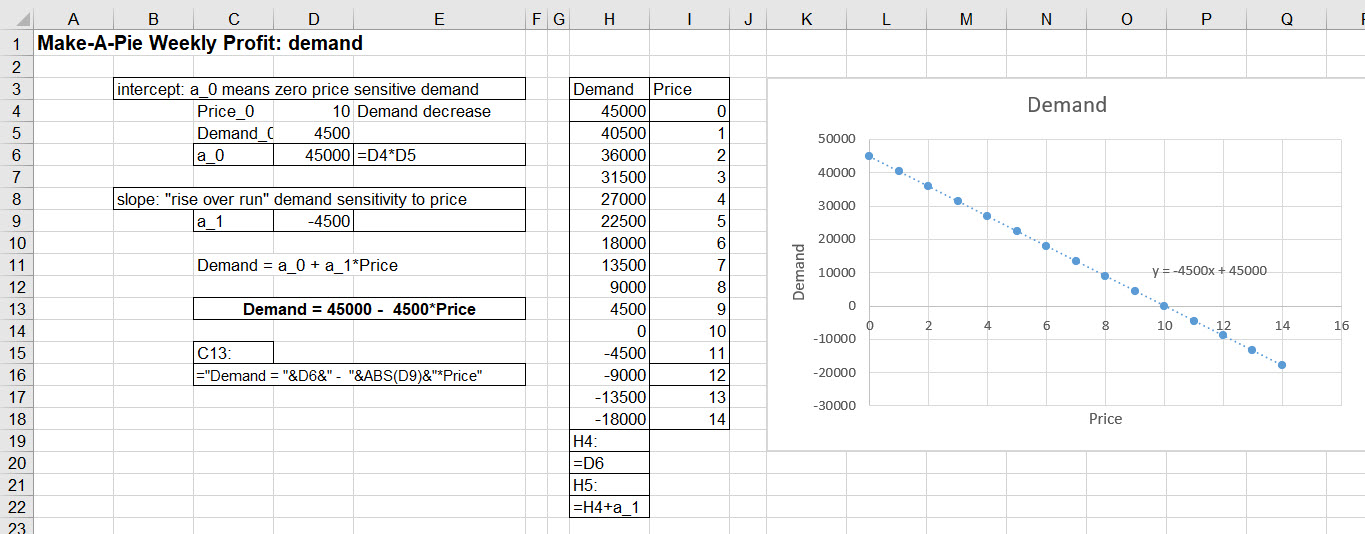
\includegraphics{images/02/pie-demand-curve.jpg}

The new conditions yield lower than previously thought volume intercept and steeper slope to meet the zero demand price of \$10. Consumers are definitely feeling the pinch in their household budgets. Grocery stores, responsible for handling, storage and insurance have increased their markups as well.

\hypertarget{a-new-profit-dawning}{%
\subsection{A new profit dawning}\label{a-new-profit-dawning}}

All of this yields a new weekly profit calculation and sensitivity analysis.

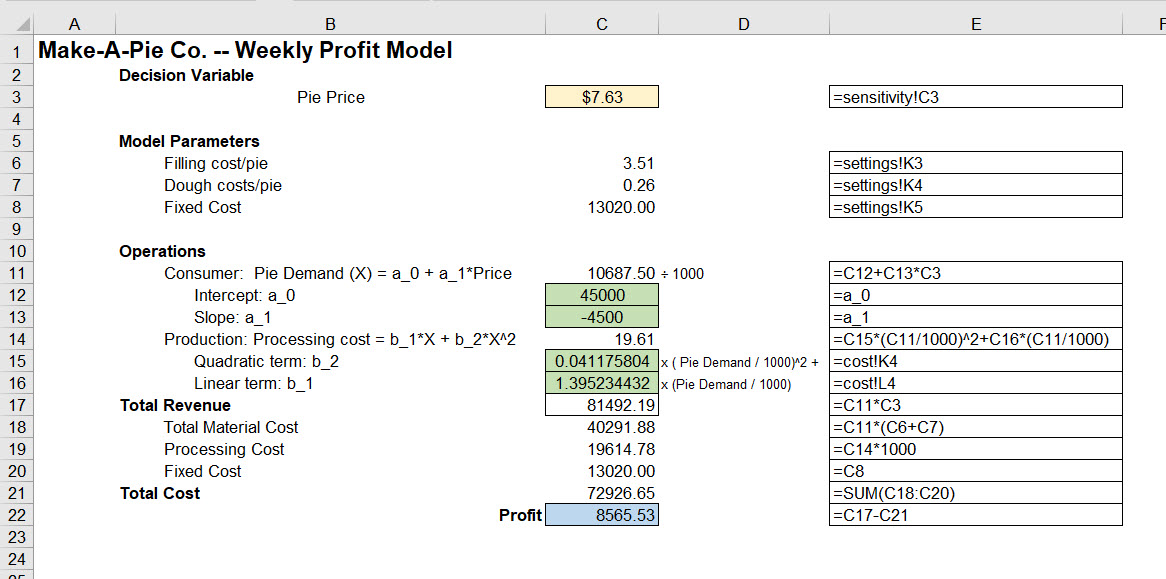
\includegraphics{images/02/pie-profit-calc.jpg}

Cells drive in from source worksheets. Notably the C3 price comes from the price sensitivity analysis worksheet.

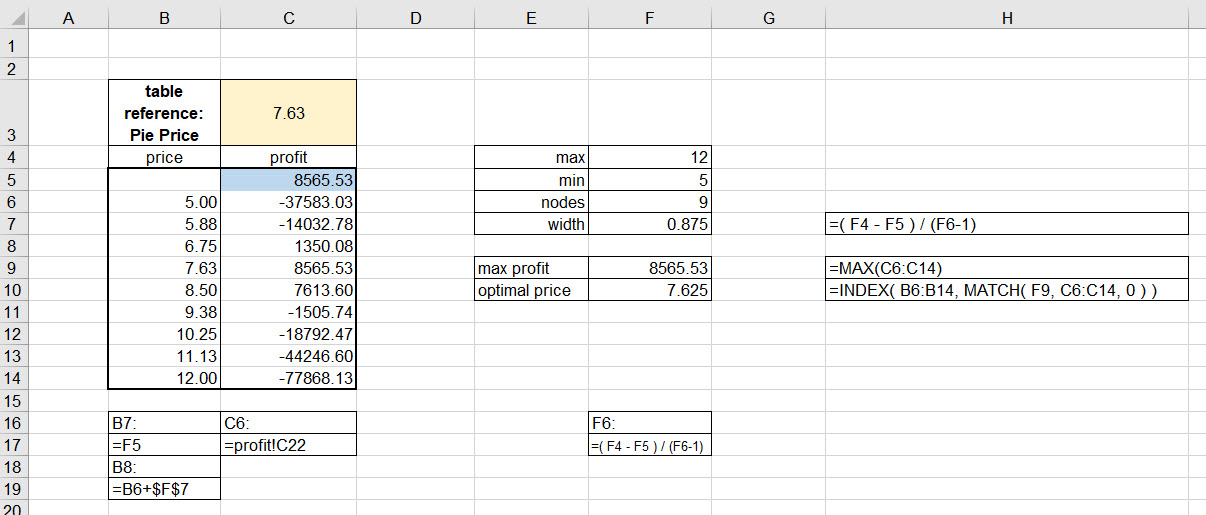
\includegraphics{images/02/pie-sensitivity-profit-result.jpg}

With these settings, Tortiere smiles at the weekly profit. But she knows full well this is not the whole story.

\hypertarget{an-algebra-of-pie}{%
\section{An algebra of pie}\label{an-algebra-of-pie}}

The rest of the story boils down to the relationships among variables of interest to Tortiere. She faces increased supplier costs and volatility of costs and consumer preferences. She believes her business is going under. Decisions, pricing, resources, timing, investment, must agily respond. She hunkers down with us, her analytical trusted advisors, to understand the breadth and depth of the situation.

\hypertarget{a-little-lite-algebra}{%
\subsection{A little lite algebra}\label{a-little-lite-algebra}}

First, she likes the influence diagram. Second, she wants to extend the ideas in the diagram across three years. She thinks this is a reasonable planning period. It can roll forward to future three year intervals. In her experience, three years is a cycle in her industry: feeding the hungry. The influence diagram generates this algebraic model of key relationships.

\[
\begin{align}
price_i       &= price_{set}  (1 + price_g) ^ {i - 1} \\
demand_i      &= (a_0 + a_1  price_i) * 52 \\
revenue_i     &= price_i  demand_i \\
process_i     &= (b_1  (demand_i / 52000) + b_2  (demand_i / 52000) ^ 2) (52)(1000) \\ 
doughcost_i   &= dough_0 demand_i  (1 + dough_g) ^ i \\
fillingcost_i &= filling_0  demand_i  (1 + filling_g) ^ i \\
fixedcost_i   &= fixed_0  (1 + fixed_g) ^ i \\
cost_i        &= process_i + doughcost_i + fillingcost_i + fixedcost_i \\
profit_i      &= revenue_i - cost_i \\
pv_i          &= profit_i + pv_{i+1} / (1 + rate) ^ 1
\end{align}
\]

The insight here is that the set price, \(price_{set}\), gets the ball rolling. When chosen, price feeds demand, which, in turn, drops into the determination of processing cost, filling and dough costs as well. Total revenue is price times demand. Total cost is the sum of all component costs. Profit is revenue minus cost. All of these elements are tracked from year \(i= 1 \ldots T\). In our case Make-a-Pie has a \(T=3\) year horizon.

Several variables grow across this horizon. If we set price in year \(i = 1\) to \(price_{set}= price_1 = 9.00\) and grow the price at \(price_g = 0.02\) per year, then by end of year \(i=2\) \(price_2\) is

\[
\begin{align}
price_2 &= price_1 (1+price_g)^{2-1} \\ 
        &= price_1 (1+price_g)^{1}   \\
        &= 9.00 (1 + 0.02)^1 \\
        &= (9.00)(1.02) \\
        &= 9.18
\end{align}
\]

In contrast we set \(filling_0 = 3.50\), at \(i = 0\), with growth rate \(filling_g = 0.07\) the initial 3.50 would grow to \(3.50(1+0.07)^1 = 3.57\) by the end of year \(i=1\). This amount will compound to \(3.50(1+0.07)(1+0.07) = 3.50(1+0.07)^2 = 4.007\) by the end of year \(i=2\). And as they often say in Leipzig \emph{und so weider}, and so on with the other calculations subject to growth rates.

\hypertarget{pvs-last-stand}{%
\subsection{PV's last stand}\label{pvs-last-stand}}

THe last equation builds, even better, accumulates value from one yeat to another. Here is a simple example for a two period cash flow process. We can extend it to any number of forward periods. We can also think of periods as seconds, minutes, days, weeks, months, quarters, years, decades, centuries, and we get the idea! We conceive of getting or giving out cash flows (profits? losses?) right now, date 0, next period, as of date 1, and the following period, as of date 2.

This drawing depicts the process.

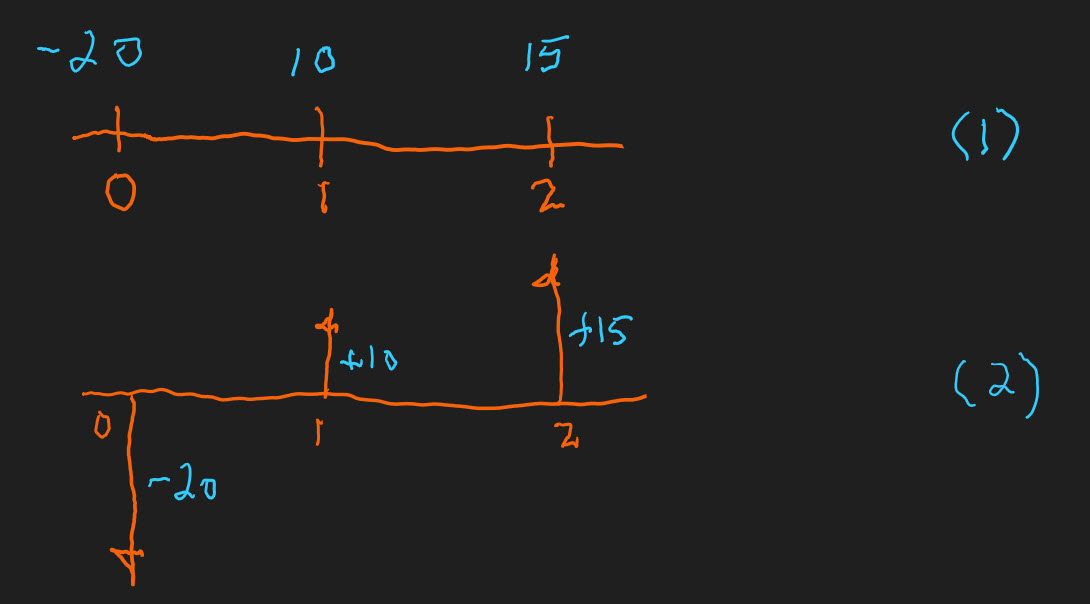
\includegraphics{images/02/pie-pv-dwg1.jpg}

Panel (1) depicts three cash flows, -20, 10, and 15 occurring at the end of each periods with dates 0, 1, adn 2. Panel (2) uses directional arrows to animate the conversation a bit. These directional arrows are frequently used in financial engineering applications and are part of the influence diagram tool-kit.

The next panel displays the calculation of the more or less obvious result that the present value of -20 paid out today is just that, -20.

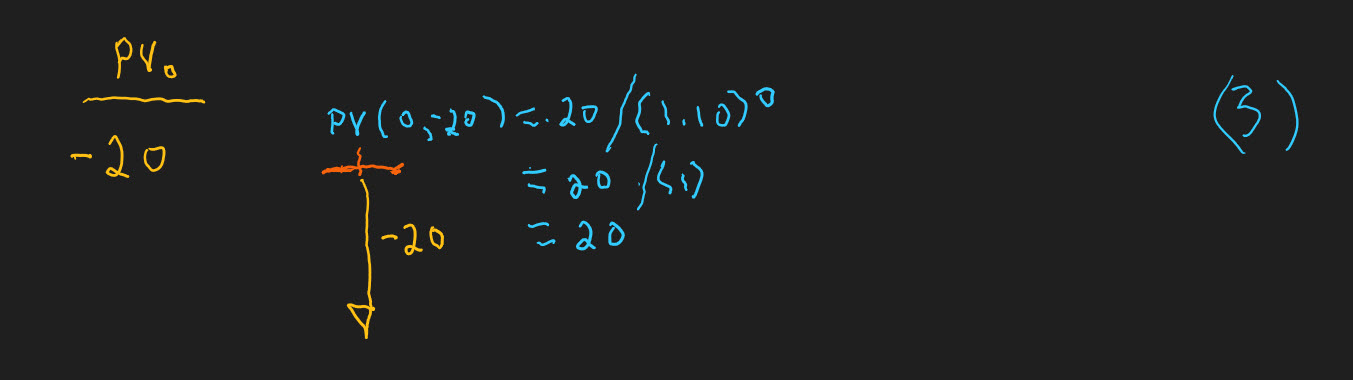
\includegraphics{images/02/pie-pv-dwg2.jpg}

We notice the discounting mechanism at work here. We calculate \(-20/(1+0.10)^0\) and realize that anything raised to the zero power is just 1 and a thing times 1 is just the thing itself. Very philosophical.

This next panel shows a calculation of the present value of a cash flow in one period. In fact this is the kernal of all discrete cash flow present value calculations. It is all we need to know for any number of cash flows. Here it is.

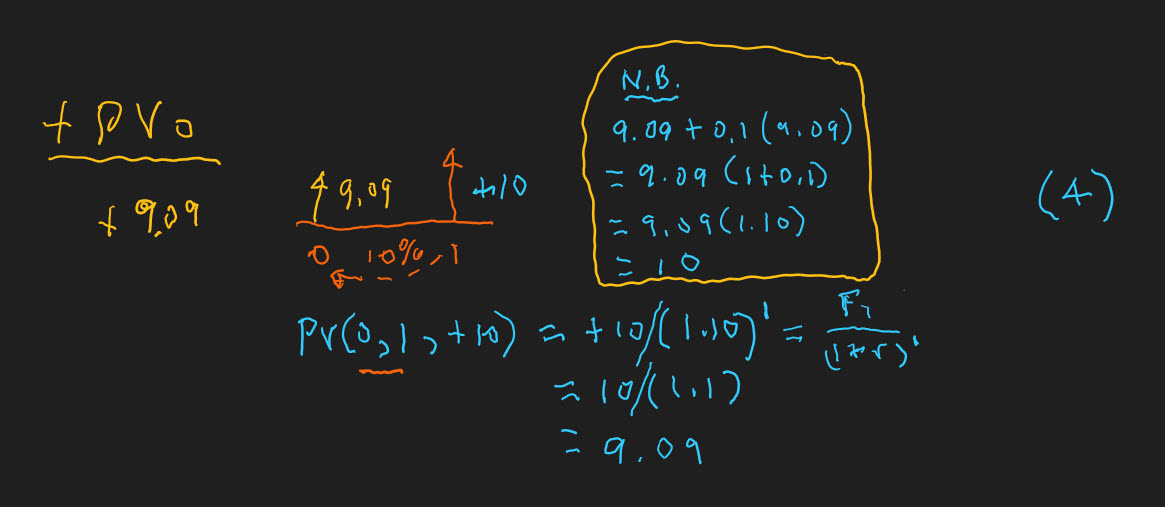
\includegraphics{images/02/pie-pv-dwg3.jpg}

We discount 10 by 10\% as \(10/(1+0.10)^1\) to get 9.09. The \emph{N.B} (that is, note well) comment works the process in the other direction. Post 9.09 bail at date 0 and receive 10\% return of 0.91 and the return of principal of 9.09 to get 10.00 at the end of the next period at date 1. Discounting and growth are inverse processes.

The next, and thank goodness, last panel shows that all we need is the one period present value. The tally so far includes present values of -20 and 9.09. One more plank to walk down and we are done.

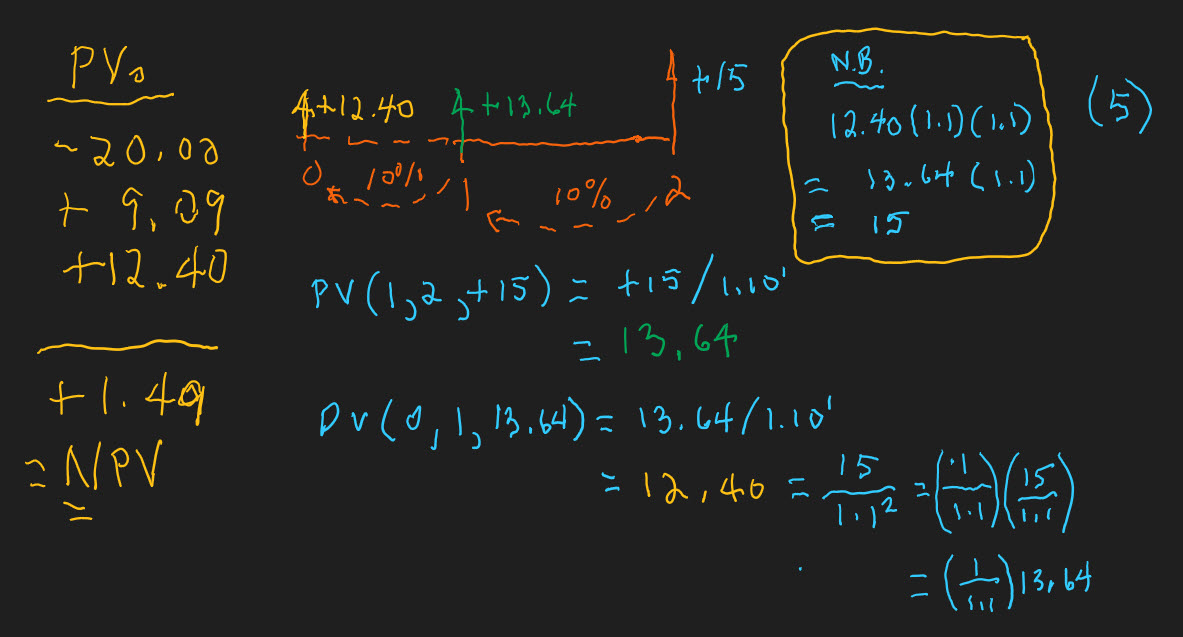
\includegraphics{images/02/pie-pv-dwg4.jpg}

A cashflow occurring at the end of two periods at date 2 is first discounted at 10\% to date 1 for a date 1 value of 13.64. Then, and if all goes well (and the creek doesn't rise!), 13.64 discounts to 12.40, again at 10\%. The PV tallies to 1.49. This is, finally, and forever more in our minds, \textbf{net present value} (NPV). NPV is just the present value of all cashflows, including today's cash flow.

Now we can add one more equation to the mix.

\[
pv_i =  cf_i + \frac{pv_{i+1}}{(1+r_{i, 1+1})^1}
\]

Any date \(i\) present value equals the cash flow occurring in date \(i\) plus the discounted present value at the next date \(i+1\) at a rate of return that is expected to occur from date \(i\) to date \(i+1\). This is powerful medicine for multi-period planning models. We will come back to this when we attempt to optimize a multi-period pricing structure for Simone Tortiere in the not so distant future.

\hypertarget{the-model-in-the-mist}{%
\subsection{The model in the mist}\label{the-model-in-the-mist}}

We will let this picture of the multi-period model begin to speak for itself (so to spreak).

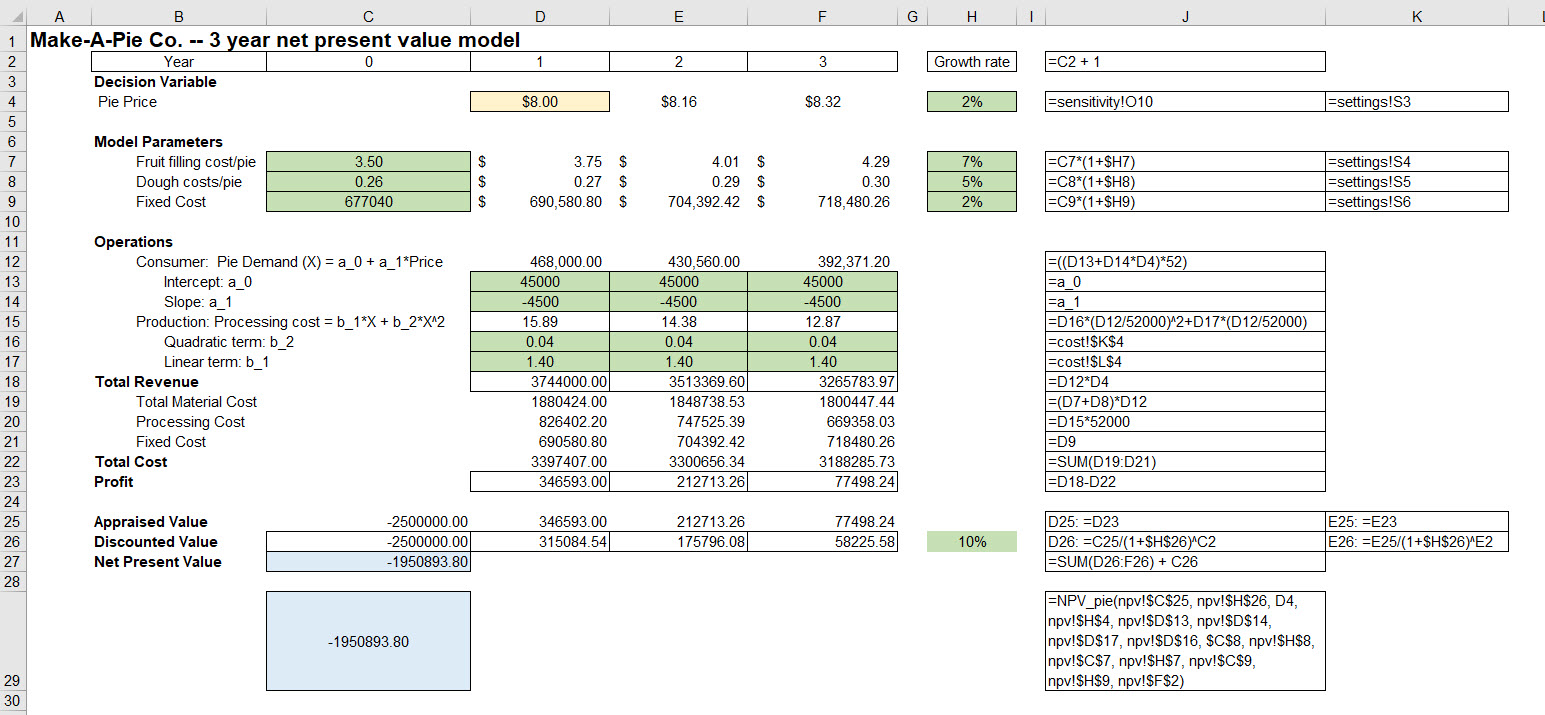
\includegraphics{images/02/pie-npv-calc.jpg}

Two things we should notice. First, the model simply is a the profit model with growth in filling, dough, and fixed costs, and let's not forget, a first year price that grows (or we can let decline). The algebraic representation maps directly into the formulae on the right. Also the price for the profit model can be set manually or comes from the sensitivity analysis worksheet.

Second, the calculation of discounted profits (really cash flow, we will have to consult with the accountants here), happens in two steps. We first calculate the discounted profit for each year. Then, second, we sum up all of the present values of cash flows (oops, profit) to arrive at the multi-period profit (cashflow) criterion we called net present value in cell C27. We do not use Excel's NPV() function for expositional reasons (showing off the full calculation) and to eliminate any confusion about the calculation.\footnote{\citet{Winston2019} Chapter 8 has many interesting details about the NPV() (and also the IRR()) functions in Excel. But if we calculate the =NPV(H26, C26:F26) we get the wrong answer, about -1,840,000. This is because Excel considers the first cash flow to occur in the first period and thus discounts the first flow by the discount rate, here 10\%. Many have done this, and some have paid the price of operational error. So why not call the NPV function the PV function? Someone at Microsoft did this a long time ago but for cash flows of even amounts, sometimes called an annuity.}

\hypertarget{how-sensitive}{%
\subsection{How sensitive?}\label{how-sensitive}}

The model computes profit sensitivity again. Here is the setup to refresh our memories of days past.

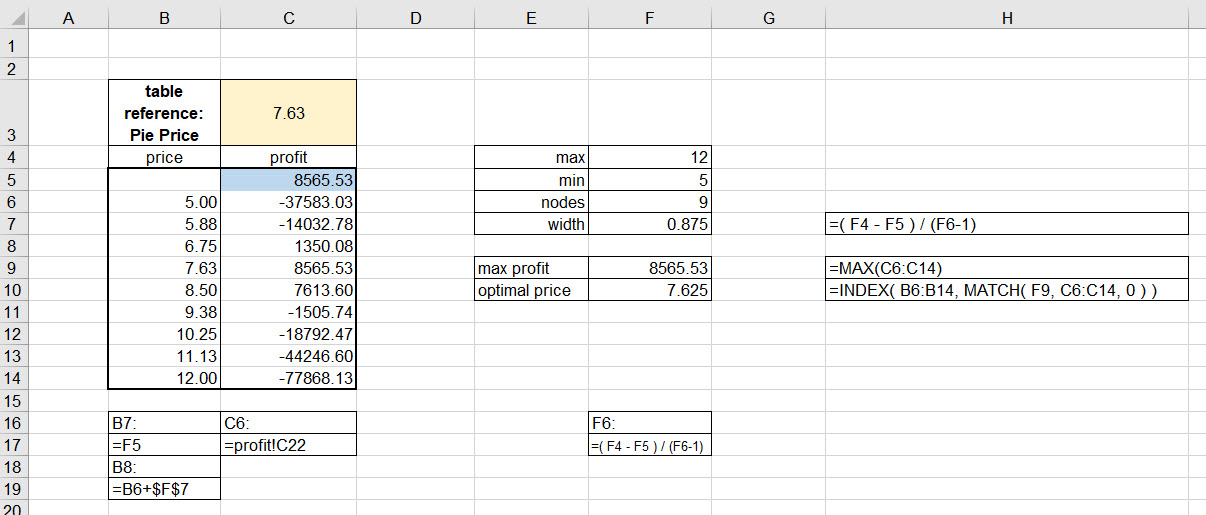
\includegraphics{images/02/pie-sensitivity-profit-result.jpg}

The Data \textgreater{} What if \textgreater{} Data Table feature comes to our aid again. We use INDEX-MATCH to locate the profit maximizing price. We plot the results for human consumers of the analysis. Here is the setup for the plot.

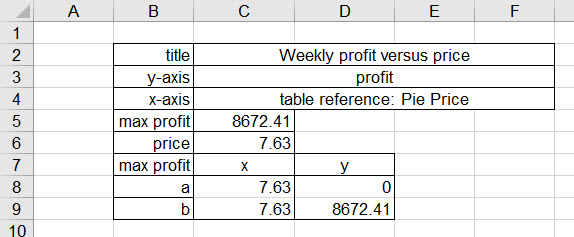
\includegraphics{images/02/pie-settings-profit-price-plot.jpg}

We locate the plot in the dashboard worksheet. This is familiar to us from the last time we met the model with only weekly profits.

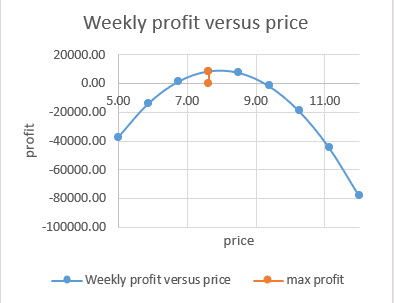
\includegraphics{images/02/pie-dashboard-profit-plot.jpg}

Done.

Well, not done. What about NPV? We perform the same tasks as we did for profit maximizing price. We use a data table to create the for loop of replacing prices in the npv worksheet with prices from the data table, and for each price calculate a new NPV. Here is the table.

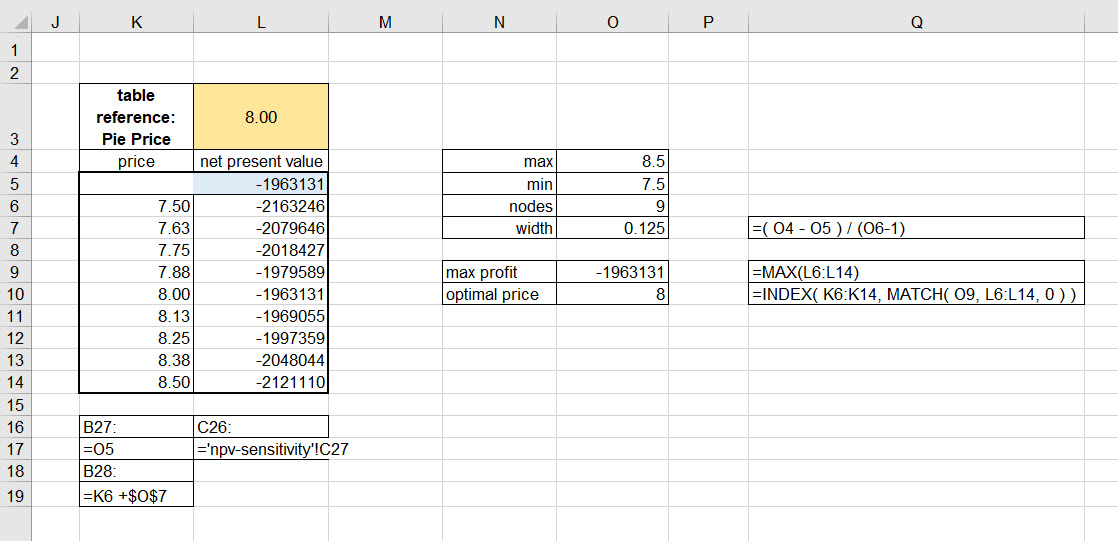
\includegraphics{images/02/pie-sensitivity-npv-result.jpg}

Of course we want to plot it. Plotting produces one more bit of information than the table: it makes very explicity the non-linear shape of profits, and multiperiod profits here labeled net present value.

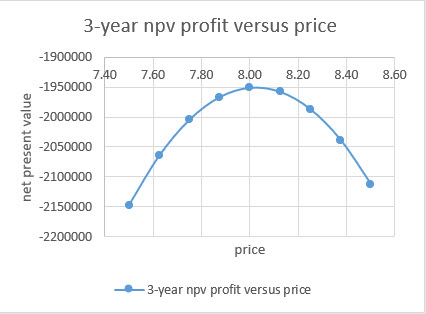
\includegraphics{images/02/pie-dashboard-npv-plot.jpg}

Oh, and one more thing, this plot dramatically shows that Make-a-Pie is under water, a quaint trope that more than suggests a uniformly, across the range of prices and for three years, a loss in the value of the enterprise. Simone Tortiere definitely furrows her brow over this rendering.What to do next?

\hypertarget{one-way-or-the-other}{%
\subsection{One way or the other}\label{one-way-or-the-other}}

We now venture into the world of a 2-way sensitivity analysis.\footnote{\citet{Winston2019} Chapter 17 shows us how to construct one-way and two-way data tables in good detail. We must always be sure to have data table reference cells in the same worksheet as the data table. In Chapter 93 he performs a many-way data table. This is a technique that easily lends itself to a spider-plot. \href{https://docs.microsoft.com/en-us/office/troubleshoot/excel/create-two-input-data-tables}{Microsoft Office help has this to say about 2-way data tables.}} We brace ourselves and strap in. First, of course, we set up a grid. This time two are two lists, here for price, and also for a variable of interest, filling cost per unit. Second, we make a grid and supply the reference for the npv calculation (from a separate npv-sensitivity worksheet to avoid possible calculation conflicts, oh my!). The references for the price and filling cost per unit on in the same worksheet as the data table. The npv sensitivity(2) worksheet does the calculations for the 2-way sensitivity table.

We call up Data \textgreater{} Table \textgreater{} What if, the row-column dialogue box appears. We choose price for the row and filling cost per unit for the column.

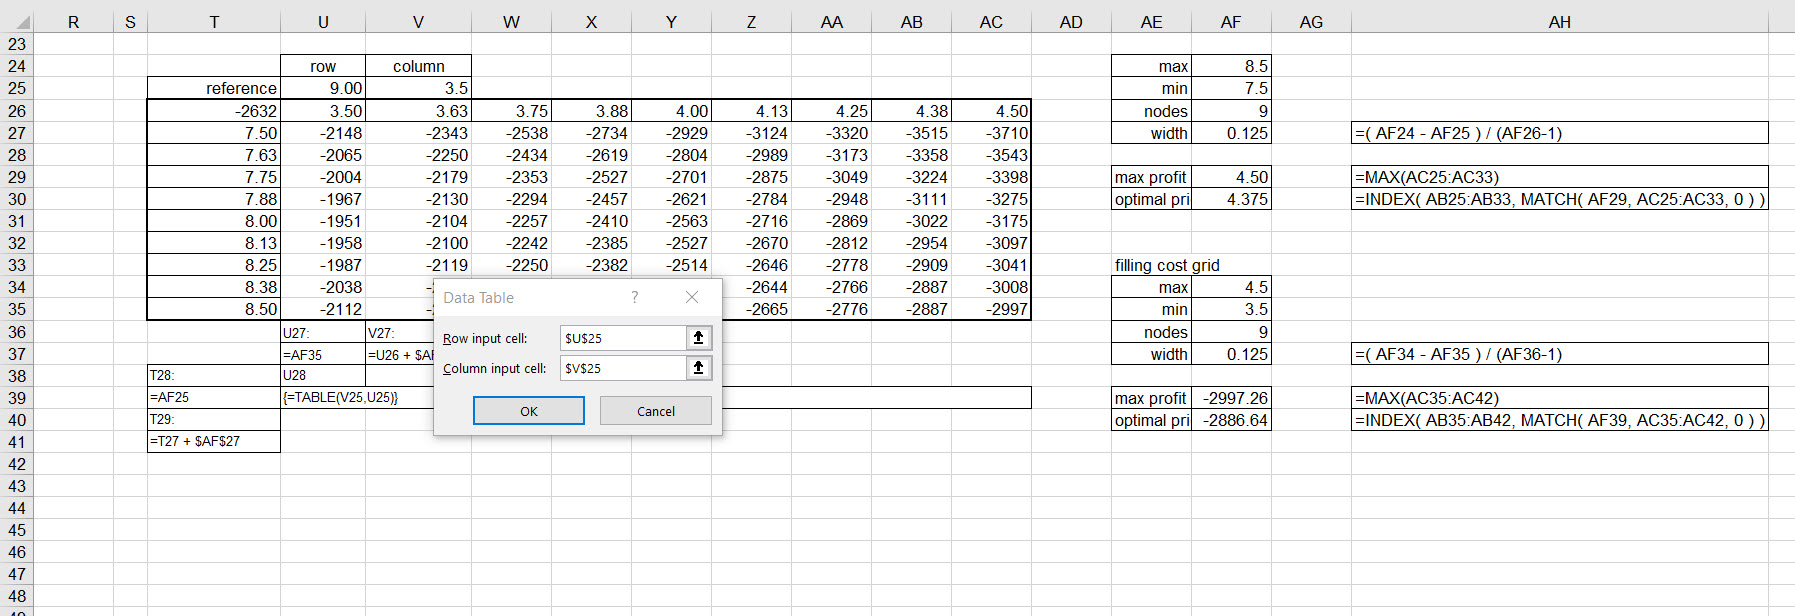
\includegraphics{images/02/pie-sensitivity-npv-2-way-data-table.jpg}

We press OK and see this table.

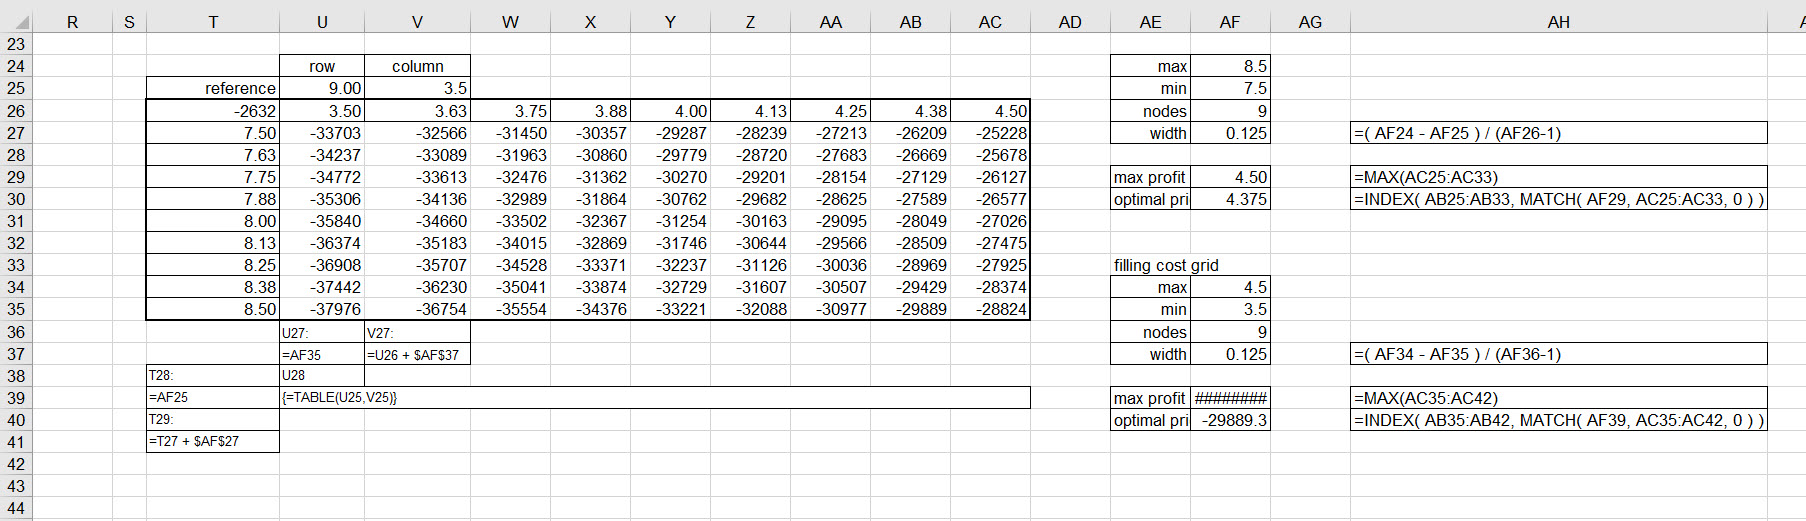
\includegraphics{images/02/pie-sensitivity-npv-2-way-data-table-result.jpg}

This took 5 seconds to run. That's too slow for a production model as we are often a bit impatient for results when under the track referee's gun to start the race! One way around this is to create our own model in Visual Basic for Applications. Here is a picture of such a model in the Developer ribbon.

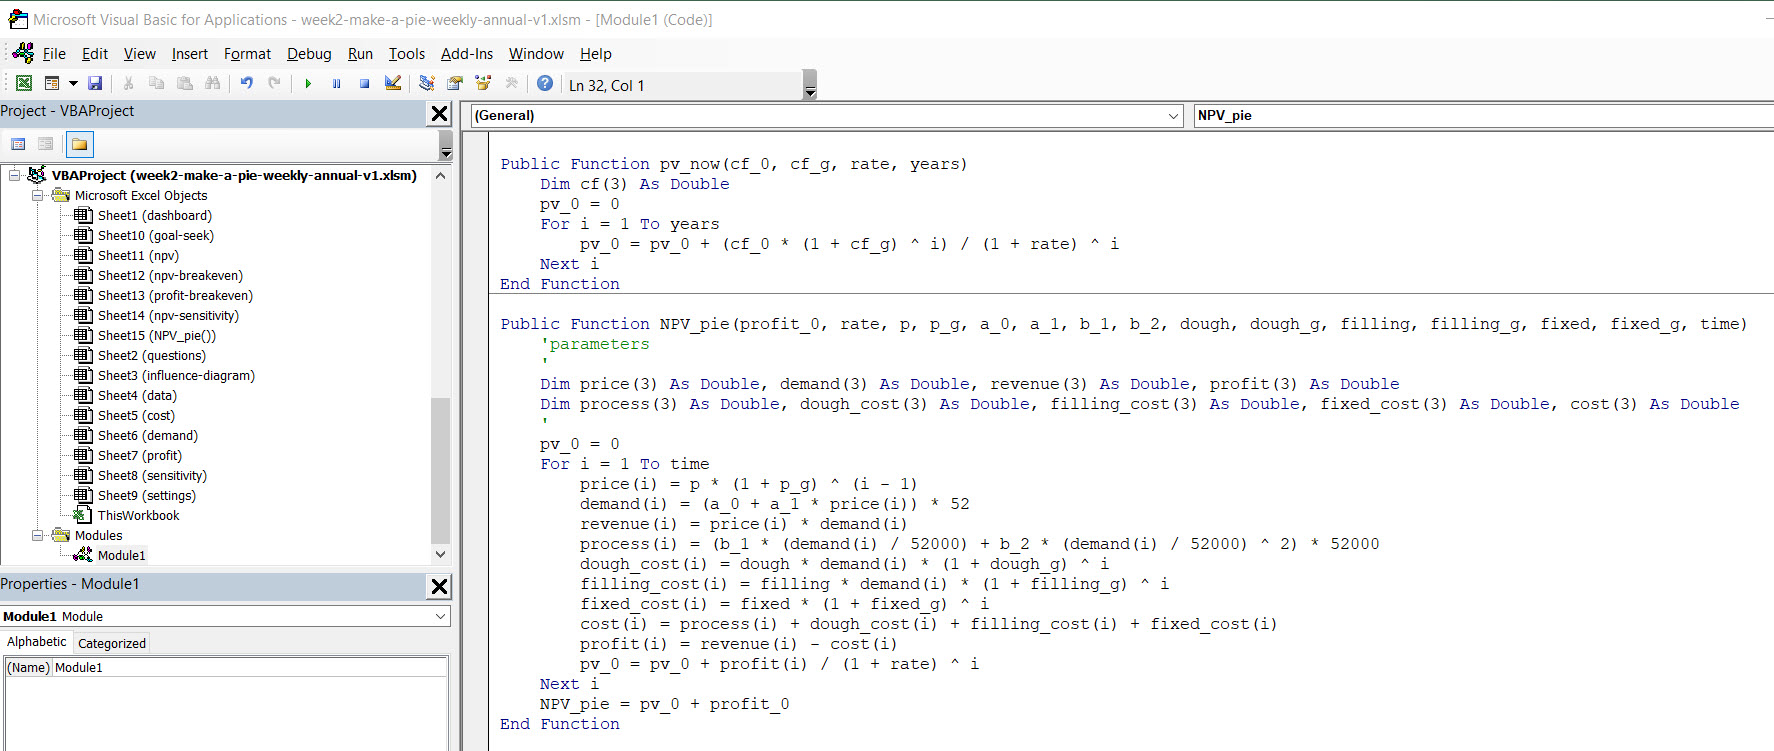
\includegraphics{images/02/pie-vba-ide.jpg}

The user-defined function (UDF) is NPV\_pie. It calculates the same value as the npv worksheet and is a good quality control check on what turns out to be a fairly complex model. The VBA function employs a FOR-NEXT loop. When we build grids like price and filling cost per unit we are implicitly using a for loop structure. We have an initial value like the minimum price. We then in the next cell increment the previous cell's value and then move to the next cell until there are no more cells to go to.\footnote{The logical thinking behind the spreadsheet seems more like the do-done logic in macro-assembler languages that underly Excel, VBA, C++, FORTRAN, APL2. \href{https://www.ibm.com/support/knowledgecenter/en/SSLTBW_2.1.0/com.ibm.zos.v2r1.bpxa400/bpxug193.htm}{Here is an IBM reference for examples.} Cell by cell calculations also seem analogous to the addresses in processor memory registers. \href{https://www.cs.virginia.edu/~evans/cs216/guides/x86.html}{Here is an example for x86 Intel processors.}}

Here is an illustration how we can use a function, or for that matter any formula, in a two way table (simply two inputs to the formula or the function). Suppose that we have the normal distribution describe cost behavior. We propose several values of the mean \(\mu\) and standard deviation \(\sigma\). We want to relate a mean with a standard deviation as if a scenario, just like a price and filling cost per unit combination. The formula for the Gaussian (normal) distribution is this beast.

\[
Pr( x \mid \mu, \, \sigma) = \frac {1}{\sigma {\sqrt {2\pi }}}e^{-{\frac {1}{2}}\left({\frac {x-\mu }{\sigma }}\right)^{2}}
\]

where \(d\) is some sort of data we are considering, say, \(d = 9\). We ask this question: \textbf{How plausible is it to observe a price that is \$9.00 per pie when when the mean and standard deviation are different values, and, this is crucial, we believe that price observations in general follow a Gaussian (normal) distribution?}

A data table comes to mind, of course! We set up \(\mu\) and \(\sigma\) grids, reference this beast of a formula, copy and paste into cells in Excel's memory caches, for example, like this rendering.

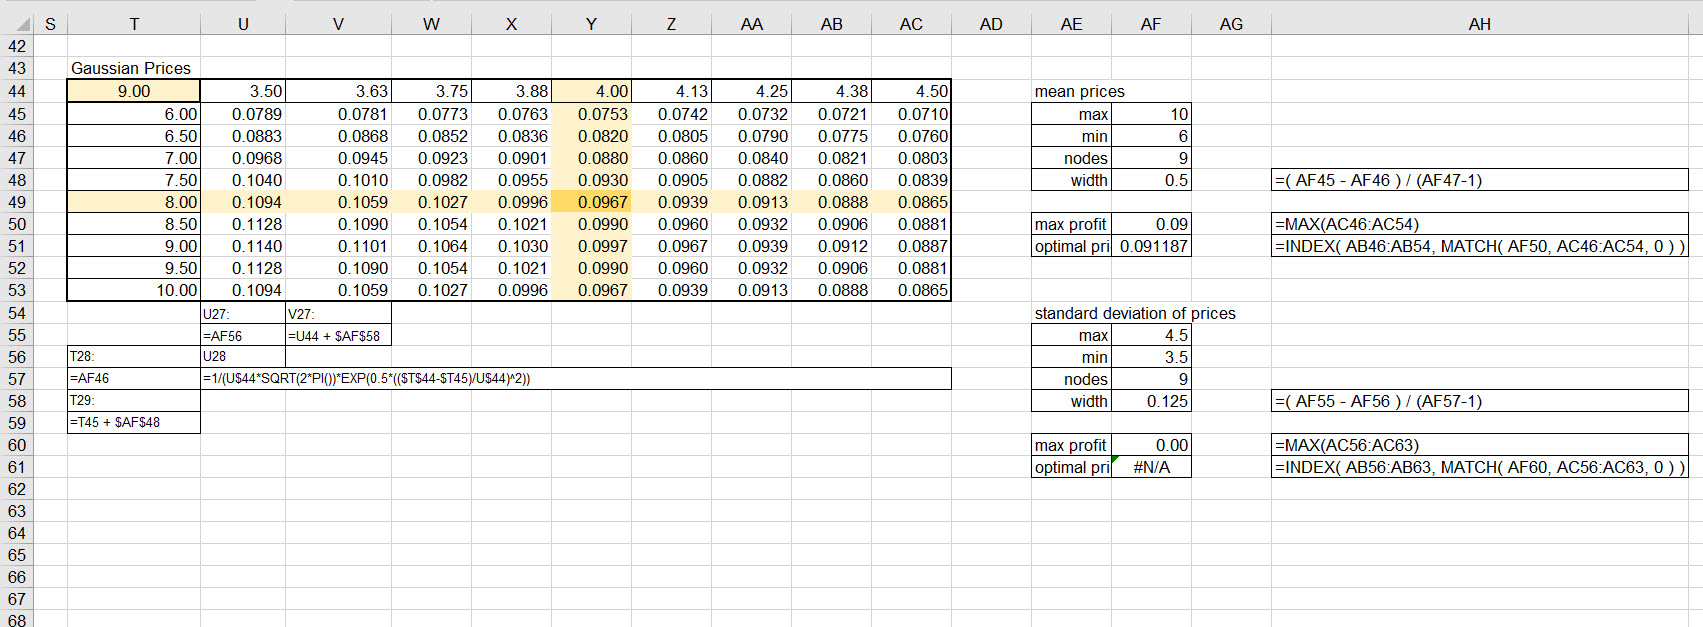
\includegraphics{images/02/pie-gauss-mu-sigma-table.jpg}

Instead of the Gaussian beast, we could have used the Excel NORM.DIST() function (with the last parameter set to FALSE for the probability mass calculation for which we clamor.) And instead of that we use our own, bespoke, NPV\_pie() function.

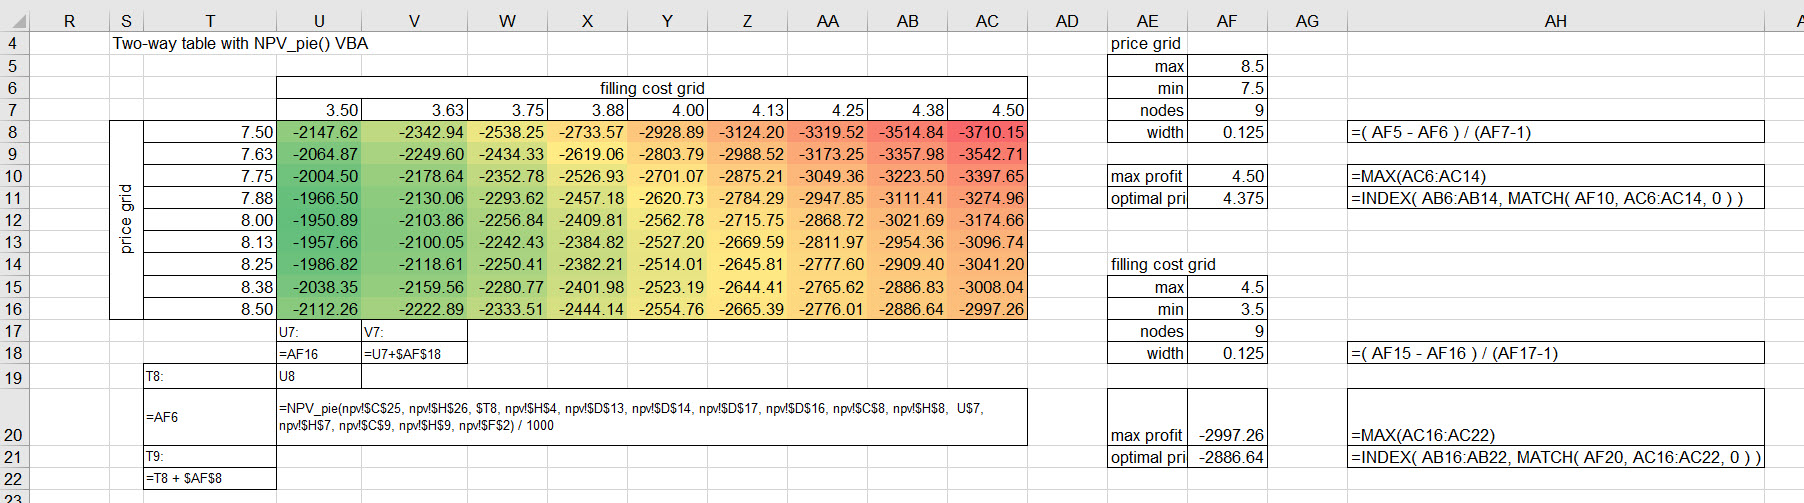
\includegraphics{images/02/pie-sensitivity-npv_pie.jpg}

And oh yes we selected the table results and at the Home \textgreater{} Conditional Formatting button selected Color Scales \textgreater{} Green-Yellow-Red. We have the notorious heat map. Use of heat maps for performance and heat map discussions are notorious because some believe them to be misleading and not good practice, \href{https://www.fairinstitute.org/blog/heat-maps-dont-support-iso-31000}{as in this article by Osama Salah.} He references the \href{https://www.iso.org/iso-31000-risk-management.html}{risk management international standard ISO 31000} for support. We can, and should, have some debate over this topic.

\hypertarget{lo-and-behold-yet-again}{%
\section{Lo and behold yet again}\label{lo-and-behold-yet-again}}

This is what we have been waiting for, agina. We modified the modular nature of this spreadsheet application extensively. The dashboard worksheet interacts with all but the questions worksheet, at least in this iteration of the application. All Simone Tortiere needs to do, after paying our invoice, is to put the cursor on the slide bars that help her understand how the profit maximizing price changes with changes in the unit and fixed cost assumptions.\footnote{\citet{Winston2019} Chapter 27 has a discussion on the implementation of user form controls. These are located on the Developer ribbon at the Insert button. \href{https://support.microsoft.com/en-us/topic/show-the-developer-tab-e1192344-5e56-4d45-931b-e5fd9bea2d45}{Here are directions to show this ribbon in your workbook.}}

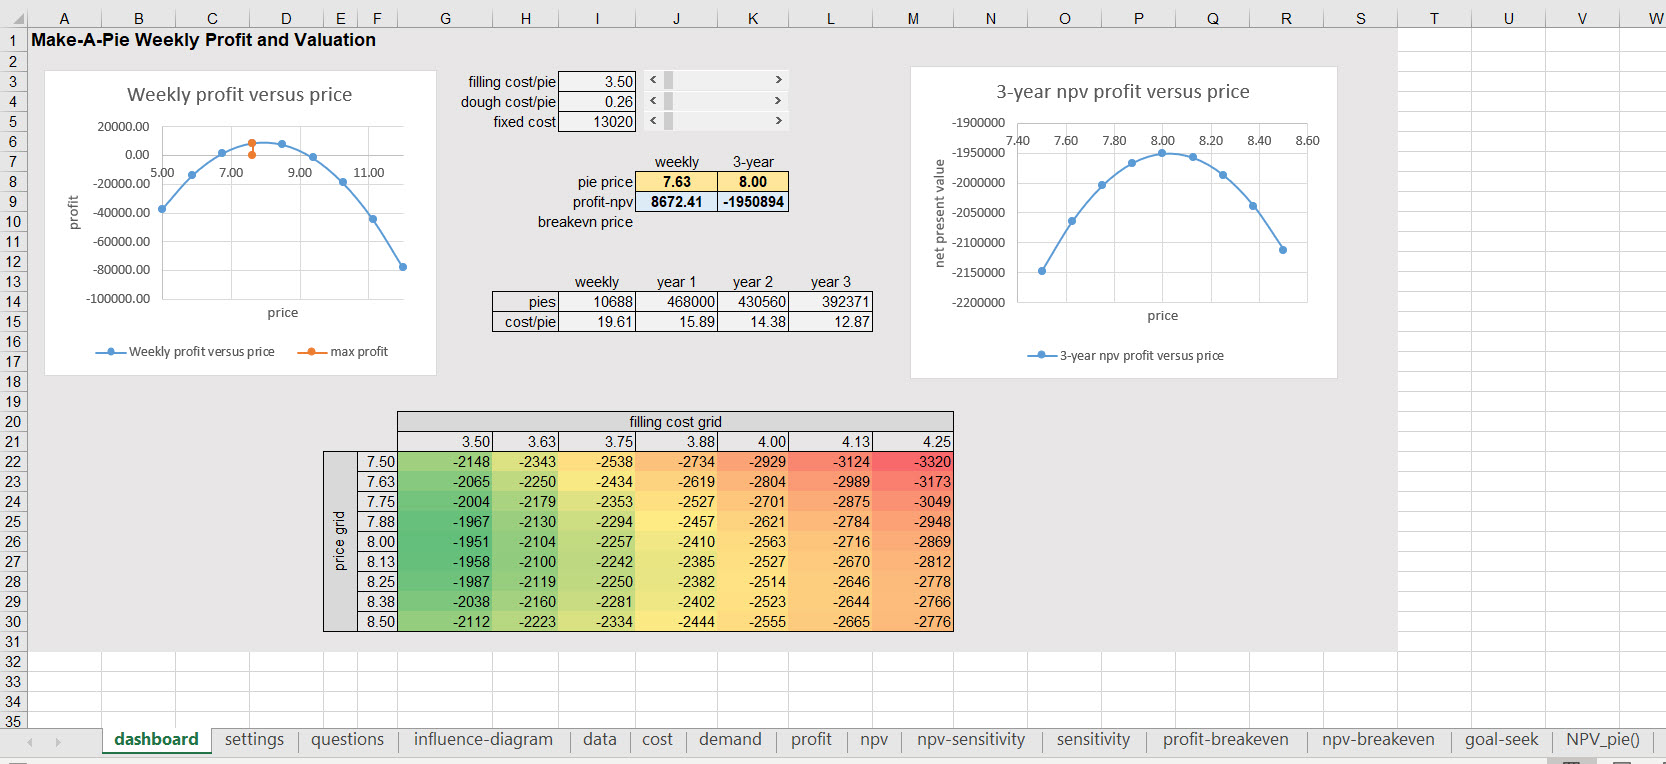
\includegraphics{images/02/pie-dashboard-all.jpg}

Is there too much in this dashboard, a question we shouldl ask Simone Tortiere? Are the colors of the heat map misleading? Only if they do not lead to a rational discussion of the lack of value in the organization, based on all of the assumptions of this analysis.

What price is best? All we have to do is live with whatever assummptions we make and read the dashboard. Using this and our beliefs about the credibility and plausibility of our results we ponder further. If enough political and emotional capital are present for a change, then change we must.

A break-even price is not even possible in this environment. If we went back to high school and solved the equation quadratic in prices that is the net present value equation we would get complex number solutions. Why? Because the NPV iceberg is entirely under water, it is negative. We would have to do something much more radical like change the structures behind the assumptions to float NPV back up to more solar energy.

\hypertarget{references-and-endnotes}{%
\section{References and endnotes}\label{references-and-endnotes}}

\hypertarget{case-salmeruxf3n-solar-systems-llc}{%
\chapter{Case: Salmerón Solar Systems LLC}\label{case-salmeruxf3n-solar-systems-llc}}

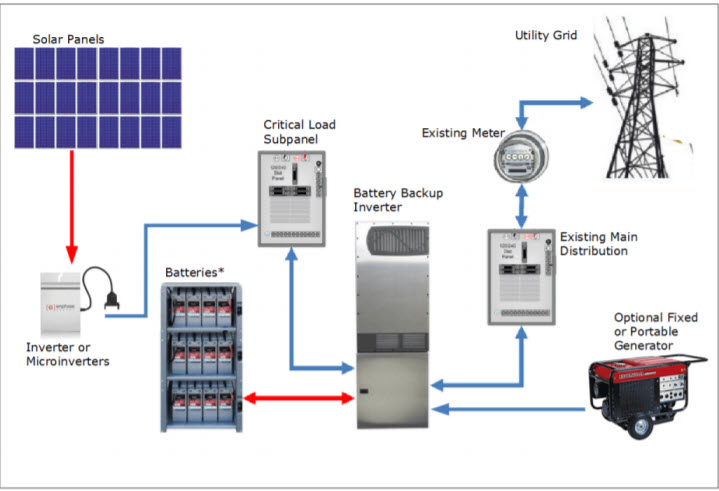
\includegraphics{images/02/solar-system.jpg}

\hypertarget{photovoltaic-systems}{%
\section{Photovoltaic systems}\label{photovoltaic-systems}}

With 50 packaged small scale photovoltaic systems already leased to industrial operators, Toni Salmerón would like to offer her US based solar leasing company for sale at a price of \$1,000,000 before the beginning of next year's operations. Tomi and her partners have built up the business over the past five years using their savings and good old-fashioned sweat equity. They hold key patents on battery, control, and manufacturing technology that they intend to retain. Toni wants us to develop a three-year economic analysis to evaluate buyers' tenders for the company.

\hypertarget{the-particulars}{%
\section{The particulars}\label{the-particulars}}

The company's property taxes are \$35,000 per year and are expected to grow at an annual rate of 4\%. Toni currently spends \$4,800 per year per system to maintain and administer the fleet. Administrative and maintenance costs are expected to increase by 7\% per year.

Currently, Toni leases her systems for \$1,000 per month each. She leases 60\% of the systems each month. Toni believes demand for her systems is highly elastic. Her market surveys and pricing experiments indicate that the percentage of the fleet leased each month increases by 7\% for each \$100 per system per month reduction in the lease price. For example, at \$600 per month, she expects that 88\% of her systems would be rented. She also believes lease prices can be increased 9\% in years two and three without affecting the fleet lease percentage established during the first year.

At the end of three years, Toni assumes for the purpose of the assessment that the buyer will resell the business for three times the revenue earned in year three. Until the end of the third year, the fleet size will remain constant so that no systems will be bought or sold.

\hypertarget{some-definitions-are-in-order}{%
\section{Some definitions are in order}\label{some-definitions-are-in-order}}

Toni defines cash flow simply as revenue minus expenses, and for this assessment will ignore depreciation and income taxes. After all, that is on the buyer in any case. She assumes that cash flow in year three includes the proceeds from the sale of the business at the end of the year and that year one's cash flow does not include the purchase price as this transaction will have happened prior to the first year in the analysis. She also defines overall investment profit as the net present value of the cash flows over the forecast horizon, assuming a discount rate of 10\%.

\hypertarget{requirements}{%
\section{Requirements}\label{requirements}}

\begin{enumerate}
\def\labelenumi{\arabic{enumi}.}
\item
  We construct an influence diagram for our analysis, labeling the decision variables, the key parameters, and the performance measures.
\item
  We then use the influence diagram diagram to construct an Excel spreadsheet. We label the cells containing the key problem parameters and constants. Our design and implementation uses named ranges, and no hard coding of constants anywhere.
\item
  We use a data table to determine the system lease price that achieves the highest overall investment performance. A graph builds on our ability to communicate results.
\item
  We then construct a 2-way data table to analyze the sensitivity of overall investment profitibility to at least one of following parameters: purchase price, annual maintenance cost/system, annual property taxes, and/or lease price growth rate.
\item
  We deposit results in a dashboard to summarize and focus a discussion around this organization/s value.
\end{enumerate}

\hypertarget{part-2-optimization}{%
\chapter*{Part 2 -- Optimization}\label{part-2-optimization}}
\addcontentsline{toc}{chapter}{Part 2 -- Optimization}

Getting our arms around

\begin{itemize}
\item
  Designing models with influence diagrams, again
\item
  Identifying the key business questions
\item
  Identifying decisions, formulating objectives, and developing constraints
\item
  Collecting data relevant to the decision framework which helps to answer the business questions
\item
  Implementing model as a linear or non-linear program
\item
  Analyzing sensitivity of results with respect to changes in decision and constraints parameters
\end{itemize}

\hypertarget{bringing-pie-to-earth}{%
\chapter{Bringing Pie to Earth}\label{bringing-pie-to-earth}}

\hypertarget{it-all-started-here}{%
\section{It all started here}\label{it-all-started-here}}

The first centuries of Islam saw the confluence of Hindu, Persian, and Mesopotamian science and mathematics. It is the algorithms that concern us here. The Latinized (translated, that is) name of Persian mathematician Muḥammad ibn Mūsā al-Khwārizmī (Persian: محمد بن موسی خوارزمی, romanized: Moḥammad ben Musā Khwārazmi; 780 -- 850 CE) is \emph{Algorithmi}- from the Arabicized al-Khwarizmi and formerly Latinized as Algorithmi. He led the research and teaching programs at Baghdad's \emph{Beit-al-Hikima}, the House of Wisdom.

Central to our purposes, Al-Khwarizmi wrote and compiled a procedure in \emph{The Compendious Book on Calculation by Completion and Balancing}, 813--833 CE (\citet{AlKarizmi830}) which we still use today to systematically solve linear and quadratic equations. We come across both in our work: net present value and profit both are quadratic in price, or volume. He employed both \emph{reduction} and \emph{balancing} (whatever we do to one side of the equation be must do on the other side). The algorithms we use to solve for optimal decisions depend explicitly on the procedures developed and taught, As did al-Khwarizmi, we too will use algebra and the geometrical representation of equations to describe, explain, and interpret our results.


\includegraphics{images/03/pie-2-products-arabic-algebra.jpg}

This page from al-Khwarizmi's work describes his procedure to find the largest square of 8, and of course it is 64. We will use equations, drawings, and graphs to perform much the same tasks for this menagerie of models.

\begin{itemize}
\item
  allocation models
\item
  covering models
\item
  blending models
\item
  network models
\end{itemize}

As we should always, we begin with a simple, but instructive, and even useful model for a decision maker.

\hypertarget{from-humble-beginnings}{%
\section{From humble beginnings}\label{from-humble-beginnings}}

Allocation modela choose mixes and compositions typically of competing decisions to optimize an objective (often some sort of cash flow or profit) subject to less-than or equal to constraints on capacity and availability of a resource. Examples include product and sales mix, vendor mix, and team member compositions. Resource constraints often dictate a trade off among alternatives.

Make-A-Pie (MAP) produces two kinds of pies: savory and fruit. Each product requires some labor in procurement of ingredients, assembly of pies, and baking. MAP sells pies through a local distributor as well as by contract to grocery store chains. These marketing channels estimate maximum potential sales for each product in the coming quarter. The MAP accounting department calculates profit contributions for each product. The decis **ion problem is to determine the product mix which maximize MAP"s profit for the quarter by choosing production quantities for the savory and fruit pies.

We ask three questions.

\begin{enumerate}
\def\labelenumi{\arabic{enumi}.}
\item
  \textbf{What are we deciding?} We need to set product mix. These are the volume of pies to be produced. There will be many possible, feasible alternatives from which to choose. For MAP the decisions are just the number of savory pies and number of fruit pies.
\item
  \textbf{What is success?} We next define a performance criteria against which we measure the impact of our decision alternatives. In many organizations, the criterion is profit, or net cash flow, or net present value of benefits, costs, and risks to performance. At the least we will need to know the contribution of decisions to profit. To that end we ask the management accountants to render profit per pie. This number when multiplied by the decision number of pies will yield the total profit of the decision alternative. We are not yet done. Our criterion is \textbf{maximize profit}.
\item
  \textbf{How is success constrained?} First of all, the decision variable themselves may have minimums and maximums. Contracting with grocery chains may require minimum volumes of on-time and in-full delivery of pies to maintain the marketing channel. Second, each process will have only so many hours of operation in a given week. The time frame of a week, of the limitations of work force, materials, and even square footage of floor space to produce all present themselves as candidates to constrain the feasible combinations of fruit and savory pie production volumes. Then there is potential demand which requires a number of fruit and savory pies.
\end{enumerate}

We have additional information from Tortiere and her CFO Marta Fazi. Adhering to good spreadsheet engineering practices we store this first report in a separate worksheet called \texttt{margin}.

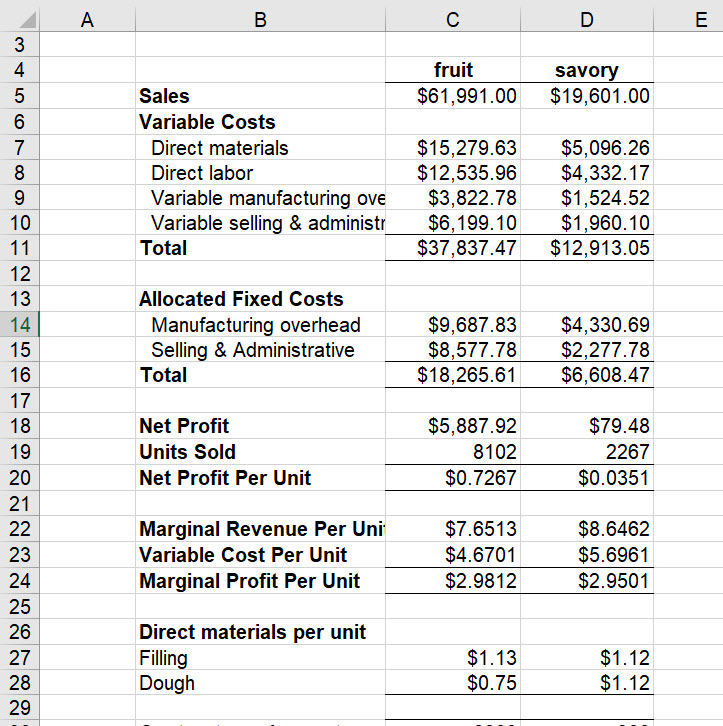
\includegraphics{images/03/pie-2-product-margin.jpg}

Marta believes that the savory line of pies is very unprofitable from a pure accounting model of value. However, she knows that allocated fixed costs must be incurred given a capacity to produce a range of the volume of pies. These expenses include environmental, health, and safety costs, general maintenance of equipment and work spaces, and even long-term employee benefits. Thus, she produced a marginal revenue, variable cost, and materials report.

We work with Marta to develop a further understanding of the business. We ask about the production process, its sub-processes, resource requirements per pie per pie line, and the availability of resources. Critical to this understanding is the way the decisions to produce pies winds its way into the underlying production processes and material availability.

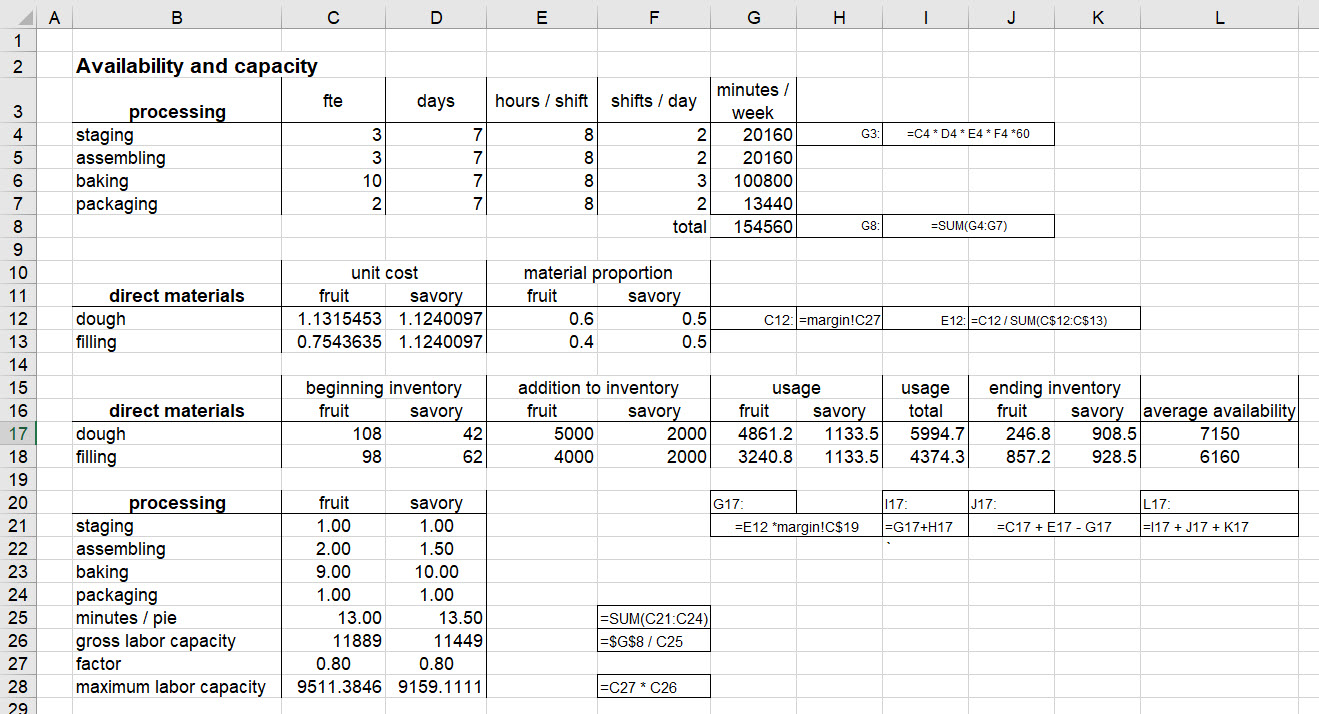
\includegraphics{images/03/pie-2-product-availability.jpg}

Marta likes the documentation using FORMULATEXT() as she trains, and educates, analysts to think through the work flow. We agree that the minutes it takes to procure, assemble, bake, and package pies is a unit of productivity measure of importance. Labor is key to the operation. The available labor minutes by activity constrains the production of pies. Adhering to good spreadsheet engineering practices we store the report in a separate worksheet called \texttt{availability}. Labor minutes of availability across pie lines is infuenced by the full time equivalent work force, number of shifts (maximum of 3 8 hour shifts), number of days (7 in a week), minutes in a day run through hours.

We model material availability through inventory. We start with beginning of the week inventory at the end of the previous week. During the week we procure ingredients thus adding to the beginning of week inventory. Then we start to use the ingredients in some proportion that is possibly different for each pie line. At the end of the week we tally up additions and subtractions to arrive at the end of week inventory. We then define material availability as beginning of week inventory plus additions to inventory procured during the week, but in advance of a production run in any shift.

\hypertarget{decisions-decisions}{%
\subsection{1. Decisions, decisions}\label{decisions-decisions}}

We attend to our first question, first. \textbf{What are we deciding?} We know we need to set the product mix. These are the volume of pies to be produced. There will be many possible, feasible alternatives from which to choose. For MAP the decisions are just the number of savory pies and number of fruit pies.

Here is a 2 dimension mapping of the decision space of all volumes of fruit and savory pies.

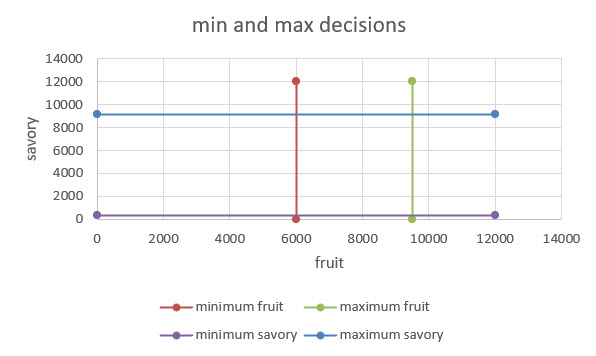
\includegraphics{images/03/pie-2-product-decisions.jpg}

First, we notice that we define decisions only in the positive quadrant of all possible combinations of fruit \(X\) and savory \(Y\) pies. Both decisions are continuous on the positive real number plane.

\[
\begin{align}
X &\geq 0 \\
Y &\geq 0
\end{align}
\]

Not only this constraint, but we also observe that there are minimum and maximum boundaries for the decisions.

\[
\begin{align}
6000 \leq \, &X \leq 9511 \\	
300 \,\,\leq \,\,  &Y \leq 9159
\end{align}
\]

Both a graph and and algebraic expression help us describe the decision space of possiblities.

\hypertarget{resources-they-are-aconstraining}{%
\subsection{2. Resources they are a'constraining}\label{resources-they-are-aconstraining}}

Perhaps borrowing too liberally from the Bob Dylan verse, we proceed to the second modeling question \textbf{What is success?} We now work with Marta and her MAP analysts to define a performance criteria against which we can measure the impact of our decision alternatives. In many organizations, the criterion is profit, or net cash flow, or net present value of benefits, costs, and risks to performance. In general this measure is multi-faceted for example when removing snow in Montreal PQ, there are competing objectives of cost and environmental impact minimization (\citet{Labelle2002}).

At the least we will need to know the contribution of decisions to profit. To that end we review Marta's profit per pie report. These marginal profits when multiplied by the decision number of pies will yield the total profit of the decision alternative. We are not yet done. Our criterion is then to \textbf{maximize profit}.

This graph depicts the family of equal-profits combinations of \(X=\) fruit pie volume and \(Y=\) savory pie volume, known affectionately as \textbf{iso-profit} curves. We can compactly express these curves using this equation.

\[
\begin{align}
aX + bY = c
\end{align}
\]

We already know what \(X\) and \(Y\) are. Coefficient \(a\) is the profit contribution per unit of decision \(X\) units (fruit pies!). Coefficient \(c\) is the profit contribution per unit of decision \(Y\) units (savory pies!). These add up to \(c\) total profits.

For example if we produce \(X=10\) fruit pies and \(Y=5\) savory prices, \emph{and} \(a=\$2.00\) marginal profit per fruit pie produced and sold and \(b=\$3.00\) marginal profit per savory pie produced and sold, then we can compute total profit \(c\).

\[
\begin{align}
aX + bY &= c \\
(2.00)(10) + (3.00)(5) &= c \\
20 + 15 &= c \\
35 = c
\end{align}
\]

Yes, it is as simple as this. The hard thing we had to do was come up with the right decisions and the marginal profits. We will use this formulation throughout our modeling work flow. We will also produce plots that will depend on the solution of \(Y\), on the vertical axis, the ordinate, in terms of \(X\) on the horizontal axis, the abscissa, of the plot. In homage to al-Khwarizmi, we balance and reduce terms to arrive at the solution.

\[
\begin{align}
aX + bY &= c \\
aX - aX + bY &= c - aX \\
0 + bY &= c - aX \\
bY &= c - aX \\
\frac{bY}{b} &= \frac{c - aX}{b} \\
(1)Y &= \frac{1}{b}(c - aX) \\
(1)Y &= \frac{c}{b} - \left(\frac{a}{b}\right)X \\
Y &= \frac{c}{b} - \left(\frac{a}{b}\right)X
\end{align}
\]

Where we used the algebraic facts that \(aX - aX=0\), \(b/b = 1\), and the distributive property of multiplication over addition. The term \(c/b\) is the intercept and the term \(-(a/b)\) is the slope of the straight-line (often called linear) equation of decision \(Y\) in terms of decision \(X\). In all of its glorious detail.

After all of that algebra in all of its glorious detail, we deserve to see our handiwork.

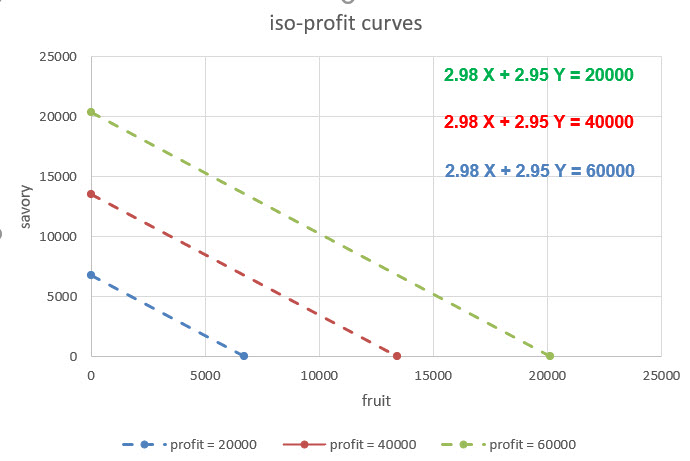
\includegraphics{images/03/pie-2-product-iso-profit.jpg}

We parameterize the iso-profit curves with three levels of profits, \$20,000, \$40,000, and \$60,000, color coordinating the equations and the dashed iso-profit lines. An increase in profits shifts the iso-profit lines to the right. Not only that, but increased profits require, of course, more sales and production of pies. The slopes of each of the iso-profit curves are the same. This means they are parallel to one another, they cannot ever cross in this slice of the decision universe.

We can measure the profit tradeoff between savory and fruit pies directly through the slope. While we might have avoided calculus in our analytics journey, or perhaps not encountered it officially at all, we can use it to think through the marginal profit tradeoff. We start with the total change in profit \(dc = a\, dX + b\, dY\), that is the sum of the change in profit due to a change in volume of fruit pies, \(a\, dX\), and the change in profit due to a change in volume of savory pies, \(b\, dY\).

These are lovely mathematical and linear operators at work. Without the fuss of knowing exactly what all that entails, but because they are linear (and by the way smooth) operators, we can solve for the ratio of \(dY/dX\), the vauntedY profit tradeoff, when, and this is key, the change in profit is stable, that is, 0, \(dc=0\).

\[
\begin{align}
dc &= a\, dX + b\, dY \\
0 - a\, dX &= a\, dX + b\, dY - a\, dX \\
- a\, dX &= b\, dY \\
\frac{dY}{dX} &= -\frac{a}{b}
\end{align}
\]

In our case \(a = 2.98\) and \(b = 2.95\). The two pie lines are literally neck-to-neck. The tradeoff is evidenced in the negative slope. A (very small) increase in fruit pie volumes \textbf{reduces} profit by \(2.98 / 2.95 = 1.01\), just a bit over a dollar. This tradeoff is the same for any level of profit, thus the \(dc=0\) assumption. Phew!

Let's overlay the minimum and maximum decision contraints on the iso-profit curves to get some perspective and maybe another insight or two.

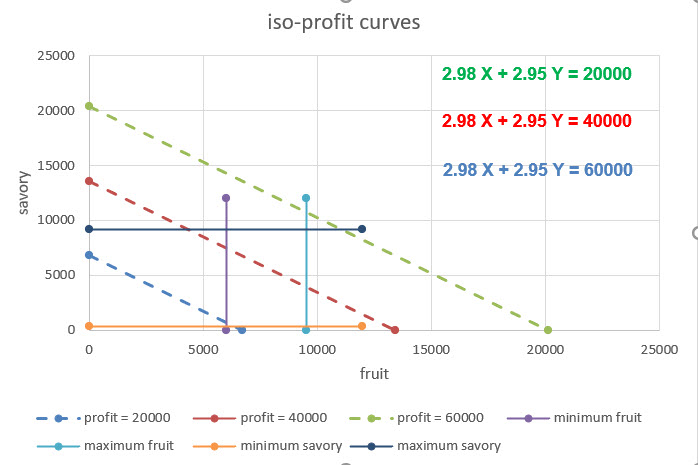
\includegraphics{images/03/pie-2-products-iso-profit-minmax-decision.jpg}

The low profit regime (\$20,000) just seems to makes it into the feasible rectangle of minimum and maximum pie requirements. The high profit regime (\$60,000) does not at all. The \textbf{decision core} will be somewhere within the feasible rectangle. One such profit is a mid profit regime of (\$40,000). Is this the optimal profit? Not yet! By shifting the iso-profit lines we must see that there is one (1) optimal, that is, maximizing profit, fruit and savory volumes solution. This plot depicts the situation.

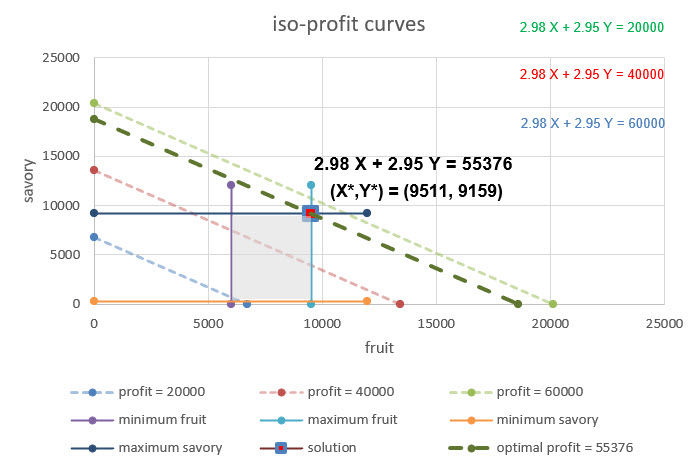
\includegraphics{images/03/pie-2-product-iso-profit-min-max-solution.jpg}

That's right, the maximizing profit decision is to produce and sell the maximum number of fruit and savory pies. This yields a profit of \$55,378. We simply moved the high profit regime line to the left to land on the northeast vertex (also known as a corner) of the four-sided polytope (also known here as a variant called a rectangle) that describes the region of feasible decision combinations. Again PHEW!

\hypertarget{not-without-constraint}{%
\subsection{3. Not without constraint}\label{not-without-constraint}}

We reach our third modeling question \textbf{how is success constrained?} First of all, the decision variable themselves may have minimums and maximums. Contracting with grocery chains may require minimum volumes of on-time and in-full delivery of pies to maintain the marketing channel. We know that this is sufficient to get at a notion of an optimized objective.

Second, each of the procuring, assembling, baking, and packaging processes will have only so many posible hours of operation in a given week. The strict time frame of a minute, an hour, a day, a week, of the limitations of work force, materials, and even square footage of floor space to produce all present themselves as candidates to constrain the feasible combinations of fruit and savory pie production volumes. Then there is potential demand which requires a number of fruit and savory pies. Even here markets, competition, communication create further constraints.

Again, we attempt an algebraic description. For the decided upon volume of \(X=\) of fruit pies and \(Y\) of savory pies, we have four (4) process resource constraints.

\[
\begin{align}
staging:\, &X + Y \leq 20160 \\
assembling:\, &2 X + 1.5 Y \leq 20160 \\
baking:\, &9 X + 10 Y \leq 100800 \\
packaging:\, &X + Y \leq 13440 
\end{align}
\]

\[
\begin{align}
filling:\, &0.6 X + 0.5 Y \leq 7150 \\
dough:\, &0.4 X + 0.5 Y \leq 6160 
\end{align}
\]
With the same results we developed for profit curves, we can find intercepts and slopes and plot these relationships. Here are the constraints for the four processes. We leave out the profit relationship for now.

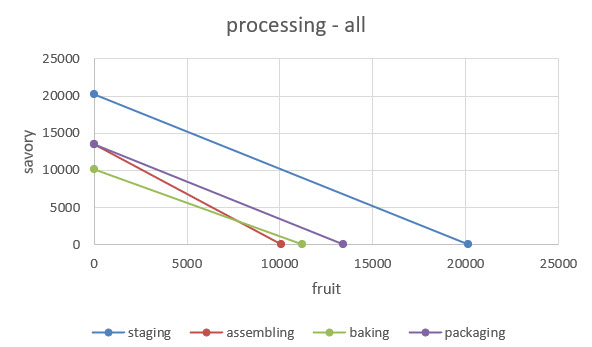
\includegraphics{images/03/pie-2-product-process-all.jpg}

We seek only the most constraining of these curves. We immediately see that both staging and packaging outstrip the assembling and baking processes. To the left of the assembling and backing process constraints lies a potential set of feasible decisions. Also we note that the slopes of the staging and packaging process constraints are the same. This adds to their irrelevance and redundancy. It is not that they are unimportant. Not at all, just not helpful in identifying the region within which decisions can be found feasibly. By feasible we then mean the decision space that fits all of the constraints. This criterion is then met only by the most constraining of the processes here.

And here are two ingredients for the material group of constraints.

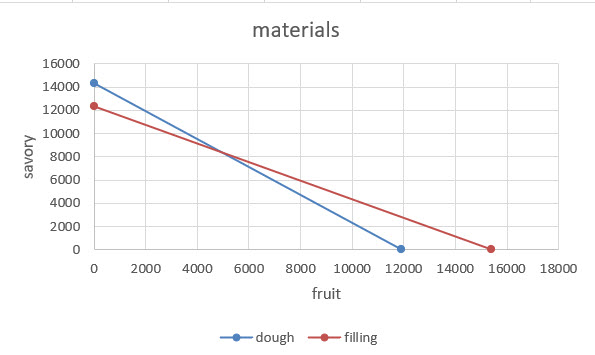
\includegraphics{images/03/pie-2-product-material.jpg}
They intersect at around \(X=\) 5,000 fruit pies and \(Y=\) a little under 9,000 savory pies. To the left of the kinked boundary at this point we may, just maybe, an optimal decision.

We now put the material constraints together with the relevant assembling and baking constraints.

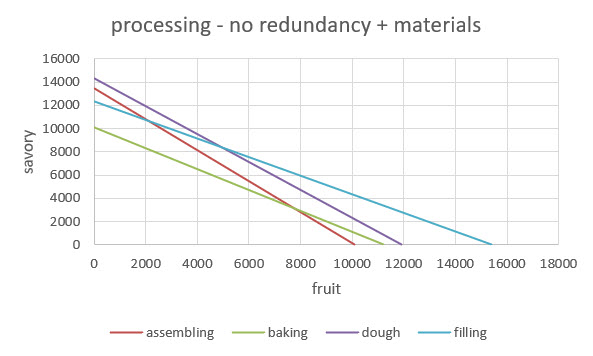
\includegraphics{images/03/pie-2-product-material-no-redundancy-process.jpg}

Wow, both of the material constraints are cut away by just the assembling and baking process constraints. Those two are the most constraining of the suite of six constraints. They alone define, along with the demand constraints, the feasible set of decisions.

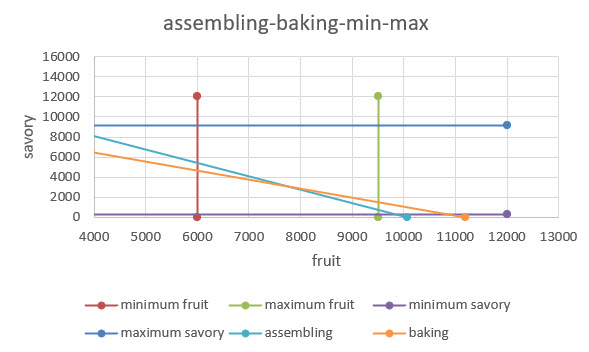
\includegraphics{images/03/pie-2-product-aassembing-baking-minmax.jpg}

That point at which the assembling and baking processes lies well within the minimum and maximum boundaries of the demand requirements. We arrive at the feasible decision space. Just one more step will get us to our goal of maximizing profit with pies!

\hypertarget{let-us-eat-pie}{%
\subsection{Let us eat pie}\label{let-us-eat-pie}}

And produce and sell it. Our sponsor Simone Tortiere and colleague Marta Fazi have followed us through this intense analysis. We are now ready to uncover the answers which we seek in this case. Here is the the final overlay of an iso-profit line through the intersection of the assembling and baking constraints.

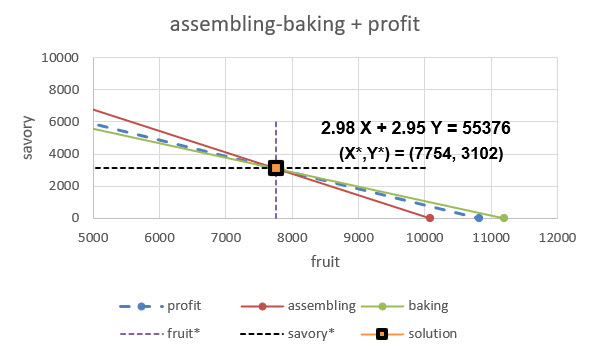
\includegraphics{images/03/pie-2-product-solution.jpg}

The iso-profit line registers a maximizing profit of \$55,376 against optimal 7,764 fruit and 3,102 savory pies. How can be know this is the best choice? First, any pie decision greater than this will be infeasible, will not honor the assembling and baking process constraints. Second, any iso-profit to the right of the dashed line will surrely be at a greater profit but then will evoke decisions that are infeasible. Any iso-profit to the left will enlist feasible decisions, but will be less profitable than the profit at the dashed line. We have found an optimizing solution, the hard way!

\hypertarget{an-easier-way}{%
\section{An easier way?}\label{an-easier-way}}

We can use the algebra of al-Khwarizmi to solve consecutively, much like the process we just followed, by eliminating, balancing, reducing constraints until we get to that one, or two, or three, or more feasible decision points. At those points we can move in the direction of increasing profit, moving the iso-profit curve to match the feasible decision point, all very geometric, in an algebraic sort of way. George \citet{Dantzig1949b} developed such an algorithm, the Simplex algorithm of linear programming.\footnote{Here is the abstract. ``Activities (or production processes) are considered as building blocks out of which a technology is constructed. Postulates are developed by which activities may be combined. The main part of the paper is concerned with the discrete type model and the use of a linear maximization function for finding the `optimum' program. The mathematical problem associated with this approach is developed first in general notation and then in terms of a dynamic system of equations expressed in matrix notation. Typical problems from the fields of inter-industry relations, transportation nutrition, warehouse storage, and air transport are given in the last section.''}

We use the Solver add-in from Excel to help us solve this problem algebraicly. We check that Excel has enabled the \href{https://support.microsoft.com/en-us/office/load-the-solver-add-in-in-excel-612926fc-d53b-46b4-872c-e24772f078ca\#:~:text=Load\%20the\%20Solver\%20Add-in\%20in\%20Excel.\%201\%20In,the\%20Analysis\%20group\%20on\%20the\%20Data\%20tab.\%20}{Solver add-in using the instructions at this site.} There are instructions for Windows, Mac-OS, and other operating systems. We find the Solver add-in in the Analysis group in the Data ribbon (way to the right!). Frontline Systems gives us \href{https://www.solver.com/tutorials}{this tutorial for using the Solver add-in, replete with examples and spreadsheets.}

We set up a separate worksheet for our decision optimization. Here is the setup.

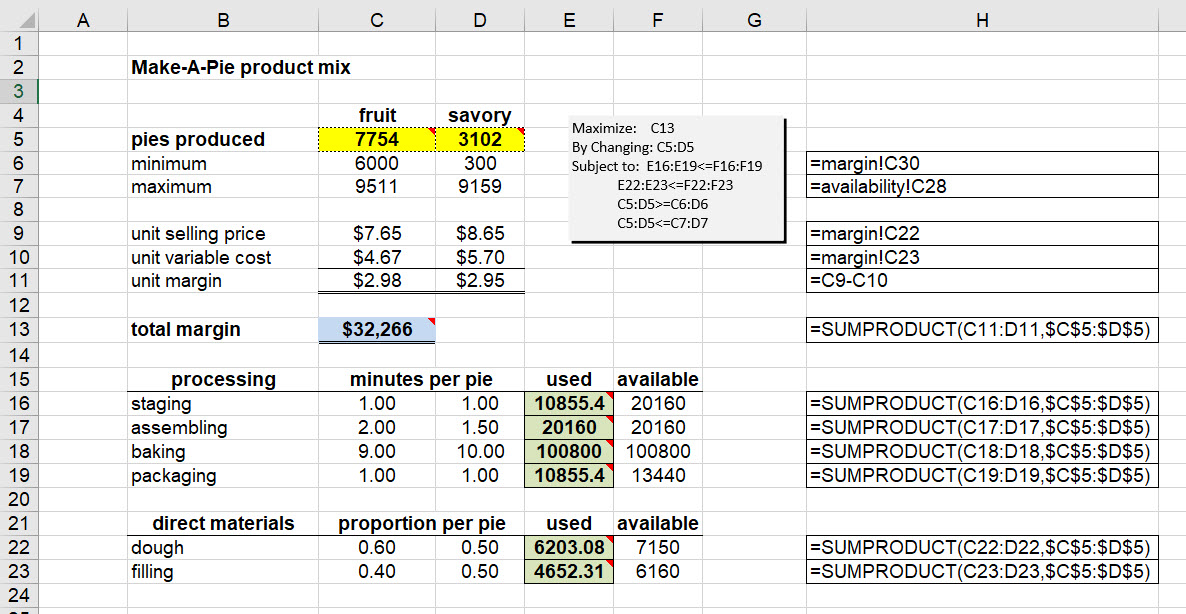
\includegraphics{images/03/pie-2-product-solver-sheet.jpg}

We color decisions yellow, criteria blue, and constraint usage green. Extensively SUMPRODUCT comes to our aid. We see the technology of pie making through the process and material constraints. The proportions of material filling and dough and the processing of the materials into pies evoke the design of each pie. We express labor and capital supply and demand, customer supply and demand through costs, availability, capacity values and constraints. This worksheet refers to other worksheets like availability and margin for values from reports and analysis.

We are ready to use Solver.

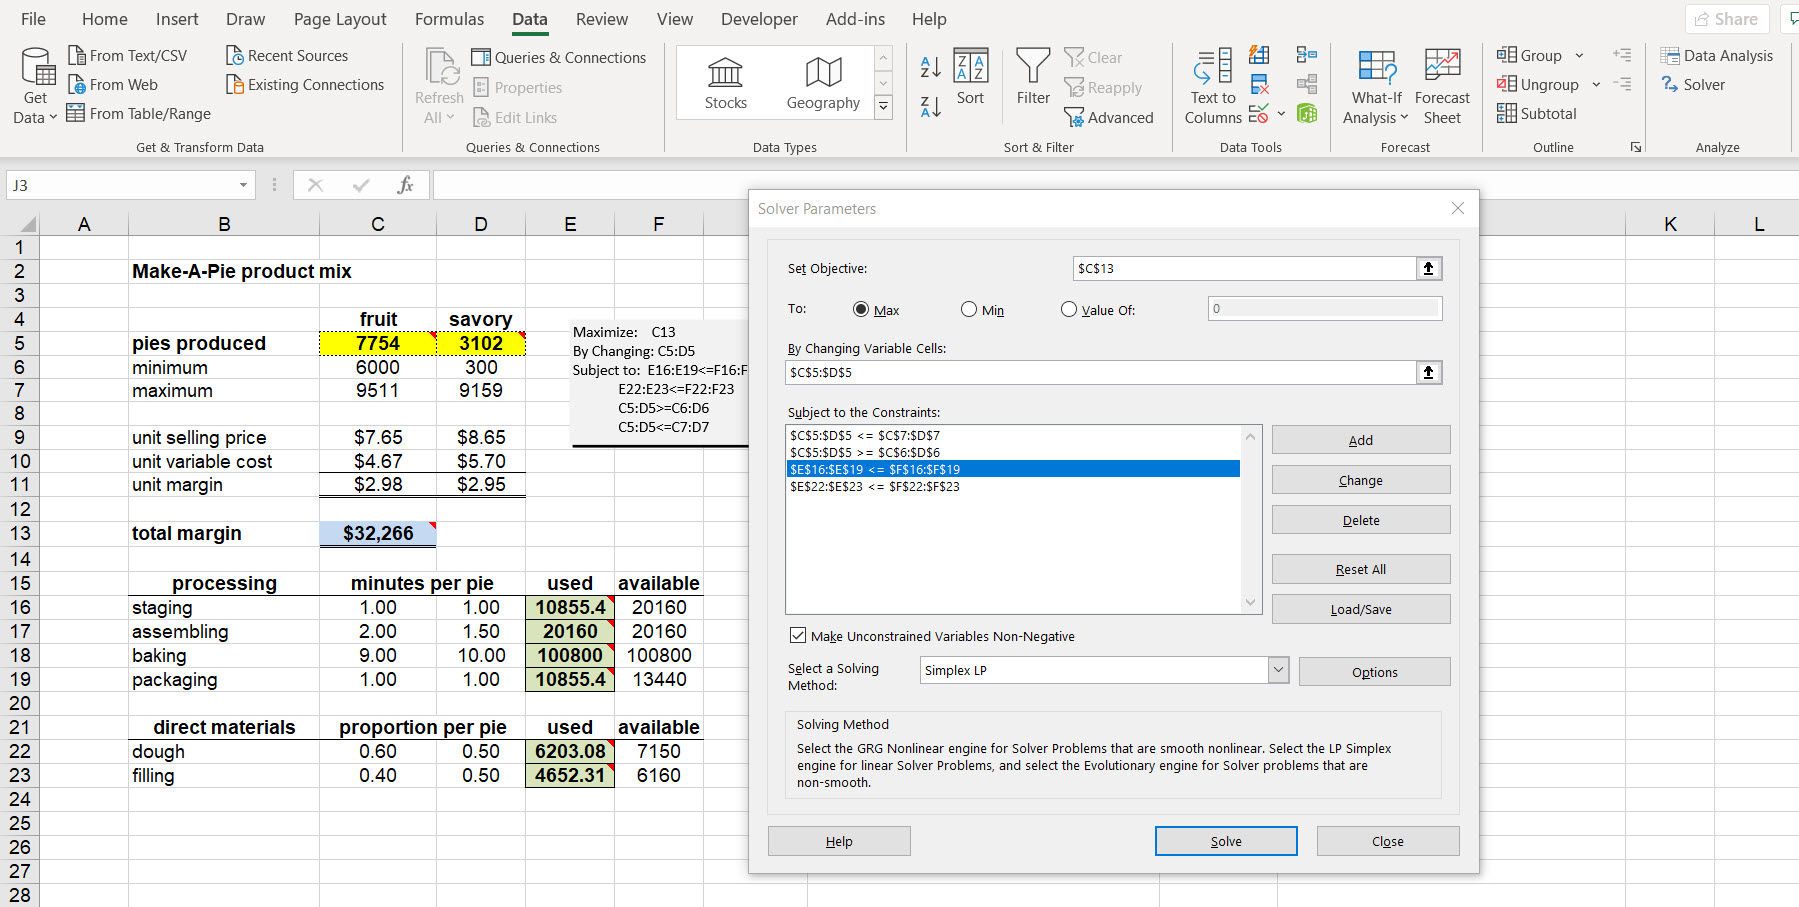
\includegraphics{images/03/pie-2-product-solver-1.jpg}

Let's look at one of the constraints, actually all four of the processing constraints. Here is how we enter and edit a constraint.

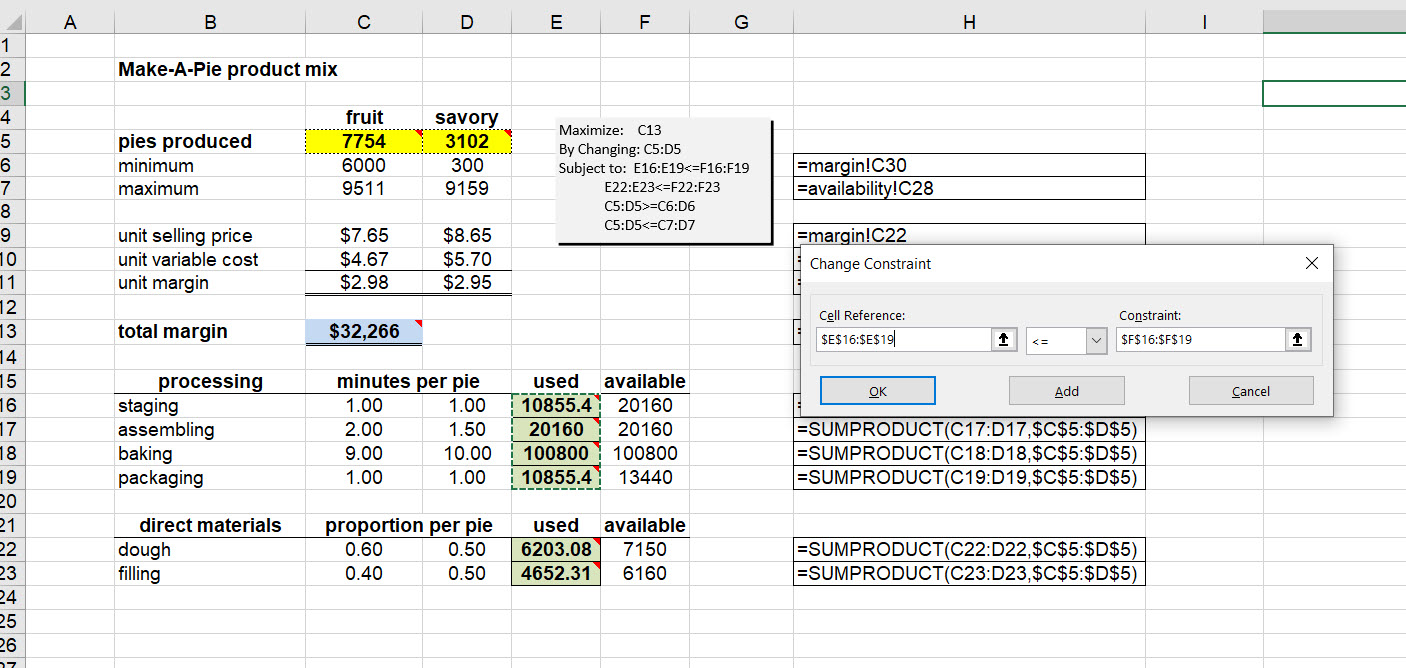
\includegraphics{images/03/pie-2-product-solver-2.jpg}

Constraint arrays can be chosen without the need to put each constraint separately. Thus the way we set up the problem with constraints in rows together, decisions in columns together, allow us this succinct way to implement the model. We press OK and go back to the main Solver dialogue. If we think we have loaded all of the data into Solver, we then press Solve.

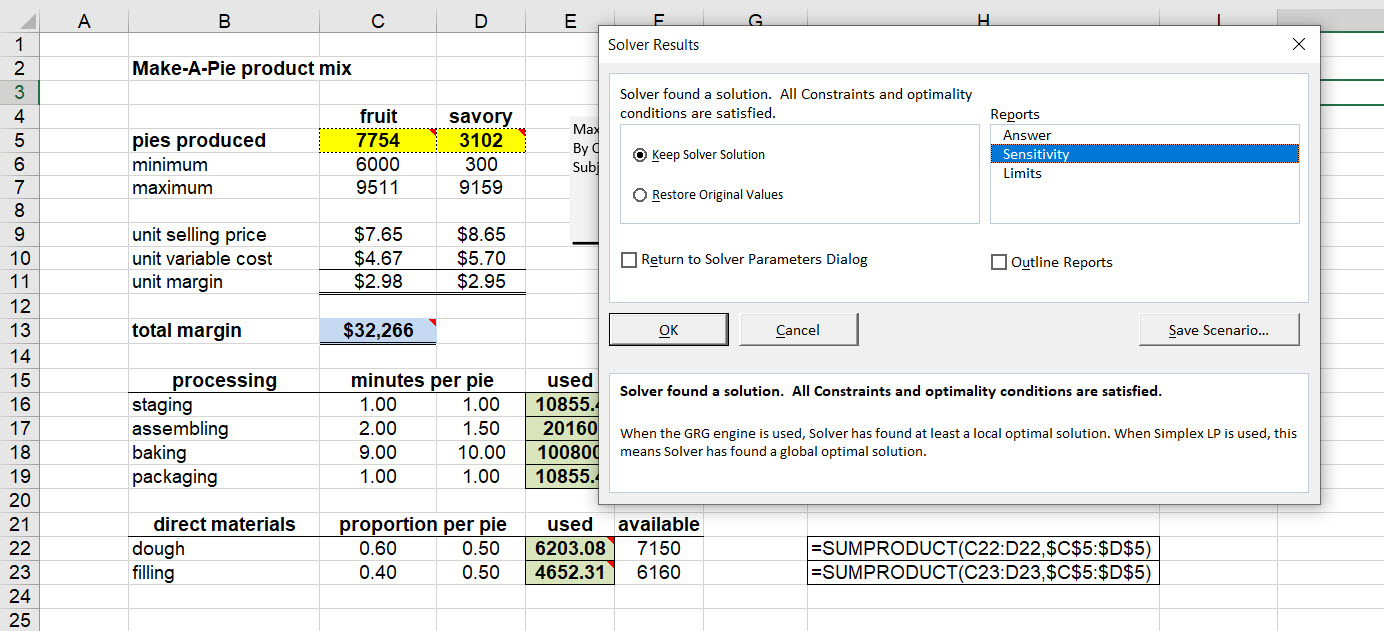
\includegraphics{images/03/pie-2-product-solver-solve.jpg}

This dialogue asks if we want to use the new solution. If yes, this will wipe out the previous solution. We also can write other reports to worksheets. Sensitivity analysis is one such report we will need. Press OK to see the solution deposited into our model.

All of this is very mechanical. Our design of worksheets definitely has that character. But design is born of principles and practice. These spreadsheets follow the logic of the algebraic model. The model and its inputs in turn follow the scope of Tortiere's and Fazi's requests, born of the need to understand the technology, markets, and competition in the markets all around pie making and feeding others.\footnote{We can visit \citet{Winston2019} for several of the tricks up his sleevers. Chapter 29 is an introduction. He follows this with chapters 30-35 for various examples of linear programming of many business problems. Other chapters in his book reveal further examples.}

\hypertarget{expanding-horizons}{%
\chapter{Expanding horizons}\label{expanding-horizons}}

\hypertarget{didos-bullhide}{%
\section{Dido's bullhide}\label{didos-bullhide}}

\includegraphics{images/04/04/dido-bullhide.jpg}

Queen Dido fled the tyrannical ruler of Tyre to found the city of Carthage. Rome later razed it to the ground, salted the earth, and to this day, the site in Tunisia is inarable. Virgil at about 21-19 BCE regaled the ruling class of Rome with its origin story, that of Aeneas, Greek veteran of the Trojan War. Aeneas landed at Carthage and into Dido's arms. Star-crossed lovers were not blessed by gods or humans, all ending in tragedy for Dido and Carthage, eventually, and the establishment of Rome by myth.

Wonderful story, but here is a formal optimization problem solved by Dido which resulted in her, and her retinue, founding of Carthage. They solved the problem of finding the figure bounded by a line which has the maximum area for a given perimeter. The solution is a semicircle. Here is a statement of the problem in Virgil's Aeneid, of course, with an engaging back story up front to keep up at the end of our seats.

``The Kingdom you see is Carthage, the Tyrians, the town of Agenor;
But the country around is Libya, no folk to meet in war.
Dido, who left the city of Tyre to escape her brother,
Rules here--a long and labyrinthine tale of wrong
Is hers, but I will touch on its salient points in order\ldots.Dido, in great disquiet, organised her friends for escape.
They met together, all those who harshly hated the tyrant
Or keenly feared him: they seized some ships which chanced to be ready\ldots{}
They came to this spot, where to-day you can behold the mighty
Battlements and the rising citadel of New Carthage,
And purchased a site, which was named `Bull's Hide' after the bargain
By which they should get as much land as they could enclose with a bull's hide.''

Well, we suppose they took the largest bull they could find and produced the longest length of leather thong they could and enclosed land area within the semicircle of leather lacing. Well, that's an optimization problem, solved!

Around 300 BCE Euclid wonders about the minimal distance between a point a line, and proves that a square has the greatest area among the rectangles with given total length of edges. About 100 BCE Heron proves that light travels between two points through the path with shortest length when reflecting from a mirror. This last optimization had psychological and metaphysical implications since the reigning theory from Plato was that light emanates from our souls outward into the world and what we see is what is reflected back to us.

Here we go this time with part two (ni in Japanese this time). In mathematical
finance, the idea of maximising a profit is, of course, very important, but it's modulated by the need to simultaneously manage the risk of loss. This all boils down to a sophisticated version of the very everyday idea of not putting all your eggs in one basket, also known as diversification.

Cervantes wrote \emph{Don Quixote} in the 1600s. Here's a useful quote.

``It is the part of a wise man to keep himself today for tomorrow and not venture all his eggs in one basket.''

Not only is diversification involved here, but also the beginnings of the notion of delayed consumption. The idea is that we might need to save for the future. Inventory is a sort of delayed consumption as well. Cervantes almost gets it. Another quote from Shakespeare expands on Cervantes (although backward in time!) the more sophisticated idea. In the Merchant of Venice, Shakespeare cleverly diversifies the asset structure of a whole estate, the portfolio, across time, when Antonio, in a conversation with his friends, told his friends he wasn't spending sleepless nights worrying over his commodity investments, and he says:

``My ventures are not in one bottom trusted, nor to one place, nor is my whole estate upon the fortune of this present year, therefore my merchandise makes me not sad.''

Hidden in there is this idea of thinking about having a balance between the near future and the rather more distant future in terms of the return on a portfolio of investments. Very nice, but how often should we diversify? Here is a heuristic from Rabbi Isaac bar Aha, in Aramaic. It's the simple equal allocation strategy, and what you should do with your wealth, you should hold a third in land, a third in merchandise, and a third, as he put it, ``at hand'', which means in cash. That is the so-called \emph{one over \(n\)} strategy. If you have \(n\) assets, you put an equal amount into each one. If you keep doing that, you're not necessarily turning over your portfolio very frequently when you move from one allocation to the other over time. Is there a Confucian version? Not necessarily, but Confucius did say that we who will not economise will have to agonise. We might think of that when we refinance, especially in tail events like the current pandemic - recession - whatever.

It is interesting that profit in prices in the NPV calculation we performed with Make-A-Pie is quadratic. When we go from the quadratic total profit to the marginal profit per unit we move to the linear. That was the big idea in optimization introduced in the 1870's by Walras. What is new now? Life is truly not quadratic! Normal (Gaussian) distributions are quadratic. Markets are not. They are not symmetric, nor are our profit decisions. They are skewed, they have outliers. We could use this for inspiration here here as we expand our horizons and dialogue with Robert Hamilton in his Introduction to Merchandize (\citet{Hamilton1777}).

\includegraphics{images/04/hamilton-quadratic-problems.jpg}

We have to remember when this was published! In this book are complete systems of trade, book keeping (double entry is the Italian approach used by Genovese bankers), probability (for annuities, pensions, forecasting), and, of course, solutions of simultaneous equations. Our task remains to build on this foundation. Our first stop will be Make-A-Pie's inventory.

\hypertarget{making-dough}{%
\section{Making dough}\label{making-dough}}

There are two outputs from the production of Make-A-Pie pies, fruit and savory pies. Our clients Toriere and Fazi want to be sure they can meet changes in demand, hold down storage and replenishment costs, save on space, and not invest too much in inventory. Quite an ask! Here is the set up.

\begin{enumerate}
\def\labelenumi{\arabic{enumi}.}
\item
  \textbf{Decisions.} Managers need to know how many fruit and savory pies to hold on hand to buffer changes in demand per week. If demand booms and production did not make enough pies, then inventory smooths the spike. If demand flags and there is too much inventory on hand, scarce short-term investment, and its financing, erodes costs and threatens profitability. With profitability threatened, plow back of earnings into the business for improvements and corrective maintenance is impaired. Is it possible to have negative and positive levels of ordering decisions? Why not, if it is possible to accept and not accept pies into inventory.
\item
  \textbf{Criteria.} Executives (Tortiere and Fazi) determine that the appropriate incentive for materials managers is the minimization of cost, without sacrificing quality of course, and numerous other constraints we will soon mention. There are several costs here. They usually are part of the \textbf{cost of carry}.
\end{enumerate}

\begin{itemize}
\item
  \emph{\textbf{Production cost}}, is assessed per unit here simply the number of pies, both fruit and savory. Working backward into the production process there would also be dough is in pounds and fillings in gallons. Make-A-Pie learned long ago to separate materials production from pie production. In fact, they own the copyrights and patents to the production of their proprietary dough and pie fillings. They then designate contract manufacturers to produce the required ingredients. Of course, Make-A-Pie audits quality daily sometimes. For our purposes, and to answer Fazi's question, we will focus on the inventory of pies.
\item
  \emph{\textbf{Storage cost}}, also called \emph{holding cost}, is also in fruit and savory pie units both per unit of time, a week in this case. What's involved in storage? Space in square footage, walk-in refrigerators, shelving, temperature and humidity control, daily maintenance and cleaning, among others, all contribute to this cost. We also should include insurance and factoring costs, both financial. There is labor too, administrative tracking, maintenance of storage facilities, cleaning, inspection.
\item
  \emph{\textbf{Replenishment cost}} occurs with any order whatever the size and is fixed per order. When inventory gets down to a \textbf{safety stock} level a **reorder point* triggers production of more pies. Demand for pies drives this cost. The demand rate is the ratio of demand to the order size, also known as the lot size.
\end{itemize}

\begin{enumerate}
\def\labelenumi{\arabic{enumi}.}
\setcounter{enumi}{2}
\tightlist
\item
  \emph{\textbf{Constraints}} are legion! At first we will not use any explicit constraints to get the classic \textbf{economic order quantity (EOQ)} model. But they will exist. One certainly is the inter-holding period constraint where we have beginning inventory, add to the inventory and use the inventory during a holding period, and net out the level of ending of period inventory. Other constraints will arise from receiving (load dock comes to mind) and storage capacities including walk-in refrigerators and freezers, shelf-space, facility availability. Still others might be an exogenously required level of \textbf{safety stock} as insurance against forced outages of supplies.
\end{enumerate}

As we should always, we begin with a simple, but instructive, and even useful model for a decision maker.

\hypertarget{model-me-an-eoq}{%
\subsection{Model me an EOQ}\label{model-me-an-eoq}}

First we draw a picture. Here is an influence diagram to help us model inventory order decisions. We might try this \href{https://online.visual-paradigm.com/drive/\#diagramlist:proj=0\&new=InfluenceDiagram}{visual art site to make an influence diagram.} Barring that here is a hand-drawn diagram on a Microsoft white board.

\includegraphics{images/04/eoq-diagram.jpg}

Aside from the scrawl all roads (arrows, that is) lead to the minimize total cost criterion for the manager. The three costs are at the next level, again, all pointing to the criterion hexagon. In this first exercise we will focus only on the pure inventory costs of storage (holding) and replenishment.

\begin{itemize}
\item
  The decision is the amount of the order in the green box, \(q_i\) for \(i=1,2\) where fruit is 1, savory is 2. If \(q_1=200\) this means that the correct number of extra fruit pies to be made per week is 200 fruit pies. This is called the \textbf{order quantity}.
\item
  Holding cost per unit \(h_i\) times the average order \(q_i/2\) across a holding period of a week feeds directly into the total cost criterion. If the total per pie holding cost of fruit pies is \$50/pie, then the fruit pie holding cost is \$h\_i q\_i = (0.60)(200) = \$ \$100,
\item
  We also have two demands driving the need for inventory, \(d_i\) for which when combined will eventually build a product mix of the two pie lines. The number of orders is the demand rate \(d_i/q_i\). If fruit pie demand \(d_1=11000\) and fruit pie order level \(q_1=200\) then the number of orders is \(d_i/q_i=10000/200=50\) replenishments. If replenishment cost is fixed at We multiply the orders by the replenish cost per order \(k_i\). This creates the replenishment cost which feeds the total cost criterion.
\item
  We leave purchase cost out of this initial analysis and give it over to the production for Make-A-Pie. We will come back to this portion of the analysis since we will eventually need to value this inventory.
\end{itemize}

The total cost function so far is this expression for each \(q_i\). Since the cost \(C_i\) for each pie simply adds together across the two pie products we really only need to look at one of the products at a time.

\[
\begin{align}
C_i = h_i\left(\frac{q_i}{2}\right) + k_i\left(\frac{d_i}{q_i}\right)
\end{align}
\]

We do not have any tradeoff between inventories of the two products in this version of the model. What determines the approximate location of a minimum cost is in the replenishment, or reordering of lot sizes, the second term. Total cost is the sum of all of the product inventory costs \(C_i\).

We can find the marginal holding and replenishment costs of \(q_i\) with this optimization. We drop the subscript to ease our notional anxieties, just for a moment. We first find the first derivatives of \(C\) with respect to \(q\). This gives us the marginal impact of a change in \(q\) on \(C\). We want to find that level of \(q\) such that the impact of a small change in \(q\) on \(C\). At this level of \(q\), in this case, \(C\) will be at its very desireable lowest possible level.

\[
\begin{align}
C &= h\left(\frac{q}{2}\right) + k\left(\frac{d}{q}\right) \\
\frac{dC}{dq} &= \frac{h}{2} - k\left(\frac{d}{q^{2}}\right) = 0\\
\frac{h}{2}   &= k\left(\frac{d}{q^{2}}\right) \\
q^2 &= \frac{2kd}{h} \\
q   &= \sqrt{\frac{2kd}{h}}
\end{align}
\]

This is the \textbf{economic order quantity (EOQ)} fabled since Ford W. \citet{Harris1913} asked how many parts should be made at one time, the economic lot size. Lot size, also known as the order size, increases with replenishment cost and demand and decreases with holding cost.

Let's take a look at a plot of holding, replenishment and total cost for \(h=0.75\), \(k=2.00\) and \(D=7000\). The economic order quantity is calculated here.

\[
\begin{align}
q^*   &= \sqrt{\frac{2kd}{h}} \\
      &= \sqrt{\frac{2(2)(7000)}{0.75}} \\
      &= 193
\end{align}
\]

And this is with rounding. When we substitute \(q^*=193\) into the total cost expression we have the minimized total cost of a lot size \(C^*=145\).

\includegraphics{images/04/eoq-graph.jpg}

Holding cost rises with order quantity in a nice straighline fashion from 0 so that the marginal holding cost is just \(h/2=0.375\) per unit. Replenishment cost is a hyperbola whose slope \(-2/q^2\) is the marginal replenishment cost per unit, a rapidly decreasing amount as \(q\) approaches the holding cost line, thereafter declining at a declining rate. Total cost is not at all linear in \(q\). The non-linearity derives solely from the need to incorporate a demand per order cost to calculate replenishment.

The optimal economic order quantity is the level of lot size where any further decrease in total cost equals any incremental or further increase in total cost, the bottom of the total cost curve. We should note that this optimal quantity occurs exactly where replenishment cost equals holding cost. EOQ implicitly takes into account the timing of reordering, the cost incurred to place and replenish an order, and the cost to store and hold product. If we constantly place small orders to maintain a specific inventory level, the ordering costs are higher, and there is a need for additional storage space. All of this sense was discovered by Ford and his colleagues.

The EOQ formula assumes that consumer demand is constant. The calculation also assumes that both replenishment and holding costs remain constant. This fact makes it difficult or impossible for the formula to account for business events such as changing consumer demand, seasonal changes in inventory costs, lost sales revenue due to inventory shortages, or purchase discounts a company like Make-A-Pie might realize for buying or making inventory in larger quantities.

\hypertarget{implementing-the-simple-eoq}{%
\subsection{Implementing the simple EOQ}\label{implementing-the-simple-eoq}}

Here is a Solver setup for the raw EOQ formula we just derived. All of the data we need is built into this setup.

\includegraphics{images/04/eoq-simple-solver-setup.jpg}

We set total cost to be minimized by choosing the two decision cells. Since this is a non-linear optimization problem, Solver uses a gradient reduction approach. This method effectively uses a smart approximation iteration to get closer and closer to an optimal solution. We need to take care here as there might be other optimal solutons. There are no constraints, yet. We press OK and solve.

\includegraphics{images/04/eoq-simple-solver.jpg}

Shown in row 11 is the EOQ formula we derived. Close enough for our purposes. We should, each week, be sure there is this amount of inventory available to manage these weekly demands, given this inventory cost structure.

The costs of fruit and savory pie inventories can be visualized with this 2-dimensional grid of contours.

\includegraphics{images/04/eoq-cost-graph.jpg}

We can locate the optimal lot sizes of fruit and savory pies somewhere in the middle of the yellow ochre blob. A brute force grid like this can be computationally and visually useful for a 2 product inventory. More products than that would be difficult if not impossible to visualize, even with our expansive imaginations.

\hypertarget{life-constrains-our-simple-model}{%
\subsection{Life constrains our simple model}\label{life-constrains-our-simple-model}}

What happens when we have only so much cubic footage of storage space. Each pie package is about 3``x12''x12". This translates into 0.25 cubic feet. We might only have so much, so we create a constraint like this.

\[
a_1 q_l + a_2 q_2 \leq S
\]

where the coefficients on the \(q\)s are the space occupied per pie and \(S\) is the available space.

Another wrinkle in the time-space continuum is financing of the inventory investment. We might suppose that Tortiere and Fazi set aside \$800 per week to cover short-term, recurring inventory investment. How they come up with that amount is the subject of a financial management course. But here is where the purchase cost enters the inventory. To value the inventory, the inventory management effectively takes in inventory from production management at least at the variable cost per pie. This first-in-first-out FIFO valuation can be assailed on many accounts, again best left for a management accounting course. Here is the constraint.

\[
b_1 q_l + b_2 q_2 \leq I
\]

where the coefficients on the \(q\)s are the variable production costs per pie and \(U\) is the desired limit on inventory investment.

In all its glory, here is the Solver setup for the revised EOQ model.

\includegraphics{images/04/eoq-space-investment-setup.jpg}

Again we press OK, but also this time in the next dialogue request the Sensitivity Report. We get this solution.

\includegraphics{images/04/eoq-space-investment-solution.jpg}

The constraints make the lot sizes smaller indeed. We should by now expect this. We notice that we have some space to spare, also known as \textbf{slack}. But we do use up our allocated investment funds for inventory.

Remember that sensitivity report? Here it is.

\includegraphics{images/04/eoq-space-investment-lagrange-multiplier.jpg}

THere is this new idea called the \textbf{Lagrange Multiplier} also known as the \textbf{shadow price.} It is zero for the space constraint since we do not use all of the space, there is some \textbf{slack.} On the other hand we use up all of the inventory investment funding. Whenever the right-hand side of a constraint is completely used, we can expect a Lagrange Multiplier to show up.

Here is a little bit more than we have bargained for. We formulate a one constraint EOQ model by minimizing the cost function with a further cost (possibly benefit) to avoid exceeding the investment constraint only. We ignore the space constraint, since we already know we have enough, and more, space to go around.

Since we only want to focus on the simplest version of this model for illustration, we train our sights on just one of the \(q\)s, again. Even so, we have introduced a new variable into our midst, \(\lambda\). We take partial derivatives of cost first with respect to \(q\), for any level of \(\lambda\), the with respect to \(\lambda\), for any level of \(q\). We end up with two simultaneous equations in two unknowns, \(q\) and \(\lambda\) when we set the partial derivatives to zero. There will be an important insight waiting for us at the end of this tunnel.

\[
\begin{align}
C &= h\left(\frac{q}{2}\right) + k\left(\frac{d}{q}\right) +\lambda(I - bq) \\
\frac{\partial C}{\partial q} &= \frac{h}{2} - k\left(\frac{d}{q^{2}}\right) - \lambda b = 0\\
\frac{\partial C}{\partial \lambda} &= I - bq = 0
\end{align}
\]

After some serious, and sometimes tedious, algebraic manipulation courtesy of al-Khwarizmi, we arrive at this solution.

\[
\begin{align}
q^*      &= \sqrt{\frac{2bkdI^2}{(b-h)I^2+2b^2d}} \\
\lambda^* &= \frac{h}{2b}-\frac{bkd}{I^2}
\end{align}
\]

Yes, these are as beastly as any other equations we might have, or hope never to have, seen. We see that investment \(I\) features prominently, as does demand. These large amounts are honed down by the marginal holding and replenishment costs. An increase in the spread between variable cost \(b\) and holding rate \(h\) will decrease the amount of the lot size needed to manage inventory.

It is hard to say whether an increase in demand \(d\) in the presence of this constraint will or will not increase lot sizes. It certainly decreases the marginal impact of an increase in inventory investment \(I\) on cost, \(\lambda\). An increase in marginal holding costs also unambiguously increases the impact of investment on total cost. For our joint space and investment constraints, an increase of investment of \$1 decreases costs by \$0.06. This seems true unambiguously as well.\footnote{If we are bold, we might calculate the rate of change of cost minimizing \(\lambda\) with respect to inventory investment \(I\). That operation guves us
  \[
  \frac{d \lambda^*}{dI} = \frac{bkd}{I^3}
  \]
  So that the rise over run of inventory impact on cost will be always negative in this model as it is inversely related to changes in \(\lambda^*\).
  We should plug some numbers into these formula. That is a great exercise for the less faint of algebraic heart among us. Toy models like this at least give us some insight into what might or might not impact total inventory cost. More constraints, more products in inventory, seemingly add to the complexity of the model, but these general relationships will continue to hold mostly.} This shadow price of inventory investment also looks like an interest rate (it is!). In fact this number is behind the use of inventory to collateralize short-term borrowing and lending operations.

\hypertarget{back-to-the-future}{%
\section{Back to the future}\label{back-to-the-future}}

Tortiere and Fazi still need to plan for the future. They have figured out with us a way to express product mix, pricing, and inventory as decisions chosen to optimize relevant objective functions subject to various constraints. They still need guidance on longer term planning. They ask now for a multi-period production planning model.

\hypertarget{bottom-line-up-front}{%
\subsection{Bottom line up front}\label{bottom-line-up-front}}

We are in luck! We have done this before. Most of the elements of such a model are present in previous models. Here is a template we can work from.

\includegraphics{images/04/multi-prod-template.jpg}

Which layout should we choose?

Here is a source-sink network representation of the model from a previous engagement.

\includegraphics{images/04/multi-prod-network-old.jpg}

\(P\) is production, \(B\) and \(I\) are inventory, \(D\) is demand, the sink. We will definitely need to clean this up. We will use it to scope out the data we need and the client's requirements at the same time.

In a network like this a common, if not also neutral, node is the source. Its links point to the 6 production periods with ranges of potential production at a production cost, or it could be profit. Networks represent flows from and to common and disparate nodes. Each edge is an amount or condition flowing. The arrows indicate the direction of flow and thus by convention the sign of an amount of flow. Graphical representations like these help us understand complex relationships like feed forward and feed back flows. We know these relationships in algebra as simultaneous equations.

At period 1 initial production along with initial inventory feed demand. What is left over from demand leaves period 1 as ending inventory at a holding cost becoming the beginning inventory into period 2. Potential production enters period 2 with beginning inventory to meet outgoing period 2 demand. Again what is left over is inventory and a holding cost to the next period node and so on to the final inventory leaving the period 6 node. The algebra of the node is arrows into a node will sign positive while arrows from a node will sign negative.

\hypertarget{tighter-and-tighter}{%
\subsection{Tighter, and tighter}\label{tighter-and-tighter}}

Here is a tighter formulation that may suit us. We forecast that customers demand \(D_1,\ldots, D_T\) be the demands for the next \(T\) periods. For our purposes \(T=6\) weeks. When we get to simulation we will assume that the \(D_t\)'s are independent random variables, and that all stockouts are backordered. We will let \(c_t\) denote the unit purchase cost in period \(t\), and let \(x_t\) denote the inventory level at the beginning of period \(t\), where a positive \(x_t\) means that \(x_t\) units of inventory are carried from the previous period, and a negative \(x_t\) is a backlog of \(−x_t\) units is carried from the previous period.

We can produce, or contract with a product to procure, \(y_t\). With these conventions then \(y_t −x_t ≥ 0\) is the size of the order, the lot size in in period \(t\) with procurement cost \(c_t(y_t − x_t)\) and an increase of the inventory level to \(y_t\). Since customers demand \(D_t\) units during the period, the inventory level at the beginning of period \(t + 1\) is then this expression.

\[
x_{t+1} = y_t − D_t.
\]
If \(y_t = y\) the loss function in period t is given by

\[
G_t(y) = h_tE(y − D_t)_+ + k_tE(D_t − y)_+
\]

We use subscripted \(+\) strokes to avoid writing this expression repeatedly.

\[
(b-a)_+ = max(0, b-a)
\]

If we take expectations as perfectly fulfilled, then our model has no so-called randomness, becomes nicely deterministic, and perhaps a little rosier, for now.

Let's bring money to the table. Economic losses include the costs of holding and setting up, replenishing, back ordering, whatever vocabulary we use, of inventory. This situation is just like the myopic, period by period, static approach we used for the economic order quantity of \citet{Harris1913}. We have finally introduced here \(h_t\) as the holding cost per unit of any positive levels of inventory on hand and and \(k_t\) as the replenishment, or some might say, the back order cost. In contracts \(k_t\) could be in a penalty or breakage clause as well. We attempt to find the policy, that is, the time path, for managing inventory from time \(t=1\) to time \(t=T\) in our formulation. If we extinguish inventory, or at least factor it out and sell it at time \(t=T+1\), then we would in that time produce more or reimburse customers for funding any backlogs.

We now formulate our multi-period production plan.

\textbf{Decisions} include the path of production, or contract production known as procurement and even tolling, \(y_t\) from time \(t=1\) to the finite horizon \(t=T\), which in our problem is 6 weeks.

\textbf{Criterion} is just to minimize costs. We must set out our criterion equation. It gets a bit messy, but says it all. For the moment we will inventory management's life on the job be very rosy indeed by the gift of \(k_t=0\). We will see that this artifice will straighten any quadratic lines.

\[
min_{y_t \geq x_t} \Sigma_{t=1}^{t=T} \left(c_t y_t + h_t \left(\frac{x_t + x_{t-1}}{2}\right)\right)
\]

\textbf{Constraints} (and oops we already have at least one buried in the criterion) include any upper and lower bounds on production, inventory (for space and funding reasons at the least), as well as the relationship between current and past inventory levels.

\[
\begin{align}
y_{min} &\leq y_t \leq y_{max} & (C1)\\
x_{min} &\leq x_t \leq x_{max} & (C2)\\
x_t &= x_{t-1} + y_{t-1} - D_{t-1} & (C3)\\
x_0 &= x & (C4)
\end{align}
\]

The first two constraints, C1 and C2, just set the stage for bounding a decision in practical life. We have only so much production capacity and so much space to store inventory. These are easy ways to express much more difficult to formulate ideas, including space and capacity decisions.

The third constraint C3 is the kicker. It allows decisions in one week to affect a decision in another week. This moves us into the much more complex realm of far-sighted rather than the myopia of the static EOQ.

The fourth constraint C4 means we have to seed the process of decision making with a beginning inventory, an initial value. If this sounds like differential equations, it is, except we use the discretization of derivatives known as differences. We will also in our implementation hold the holding cost \(h_t\) and the variable cost of production
\(c_t\) constant.

\hypertarget{implementing-the-model}{%
\subsection{Implementing the model}\label{implementing-the-model}}

We use the template, repurpose it, and input the data from reports which CFO Fazi provide. Here is a summary of her report.

\includegraphics{images/04/multi-prod-data.jpg}

We have 6 weeks in the planning cycle. A large beginning inventory seems to consume funding, space, and the attention of management disproportionately to production. Both Tortiere and Fazi realize this and want us to help pare this level down. The problem is how low? They contend that the fragility of their products requires special handling, storage, and then there is shrinkage of product in inventory. So the only way to contend with high storage costs per unit is to constrict the volume, while still meeting demand and within the constraints imposed by production. In week 3 they forecast a partial shut-down of production facilities to refit and upgrade equipment.

\hypertarget{a-revised-rendering}{%
\subsection{A revised rendering}\label{a-revised-rendering}}

In conversations with Tortiere, Fazi and their colleagues we draw this map of the model.

\includegraphics{images/04/mult-prod-network.jpg}

Sources are from production and appear in squares. Demands are sinks in triangles. They flow into and out from period nodes in circles. Each period node links to past and future adjacent nodes. They follow the algebraic model. We notice from the discussion to use the average inventory across a period to assess holding period cost. Fazi wants, for the time being, to prescind from replenishment lot sizes.

We use the report and the flow network to develop this worksheet model. Here is the Excel Solver setup.

\includegraphics{images/04/multi-prod-solver-setup.jpg}

We also notice a late request to require a \(b = 10\)\% of demand per period safety stock. This is the constraint. We use a \(\geq\) relationship since a requirement is a matter of have at least a certain level of inventory on hand.

\[
x_t \geq bD_t
\]

The request for this constraint may be result of Fazi's recent conversations with Make-A-Pie's insurance broker about the coverage for the high level of inventory investment. If Make-A-Pie internally reserves some production, the insurance policy might be able to reduce, or at least not increase, the deductible for inventory losses. In this way safety stock can act as self-insurance.

Now for the final model, and this only the beginning of our analysis.

\includegraphics{images/04/multi-prod-model.jpg}

We do not violate any constraints. We have reduced inventory and inventory cost. We have a multiperiod production plan whose path depends on past and future demand. We also notice we have almost double the warehouse space needed to fulfill demand, production, and inventory requirements.

\hypertarget{next-steps}{%
\section{Next steps?}\label{next-steps}}

Of course we will find the breaking points of this model. We can render a sensitivity analysis report, attempt to understand the range of values production, and by deduction inventory, policy can evolve. What would happen if Make-A-Pie expands to all five boroughs of NYC and Westchester and Long Island? What would happen if Make-A-Pie grows new lines of business? How would we model these questions?

\hypertarget{references-and-endnotes}{%
\section{References and endnotes}\label{references-and-endnotes}}

\hypertarget{case-pricing-production-at-make-a-pie}{%
\chapter{Case: Pricing Production at Make-A-Pie}\label{case-pricing-production-at-make-a-pie}}

\hypertarget{front-matter}{%
\section{Front matter}\label{front-matter}}

Tortiere and Fazi now want us to do the seemingly impossible? Price pie. Our job is to insert a pricing decision into the multi-period production planning model. We will use the existing demand framework from the previous chapter. We could alternatively set up a similar Salmeron Solar model? Try it for practice of course! We will try to sow up our discussions on production, demand, inventory, in short a good hunk of the Make-A-Pie supply chain. That's is and that's certainly enough! But, you know, the Salmeron multiperiod planning model might be an interesting final project. Hmmm. We will see. Next week we will hop into another problem that Tortiere faces. We will need to use simulation to help her solve it.

\begin{enumerate}
\def\labelenumi{\arabic{enumi}.}
\item
  Watch this walkthrough video. \href{https://drive.google.com/drive/folders/1IiUmsB4u3j39ve8y-wpj6WK6D8uyp1FO?usp=sharing}{You can access this video here}
\item
  Build an influence diagram with production , inventory, demand, and now pricing. This could follow the approach for the production process network.
\item
  Start from the Make-a-Pie cost minimization multi-period production model. Adding more weekly periods to the model.
\item
  Use a Make-A-Pie demand worksheet as the base for price based demand.
\item
  Make a new pricing decision row. Now be sure all of the cell calculations flow through the model cleanly, especially for price drive demand. Remember we solve for price.
\item
  Check Solver's settings to be use we have the right objective cell, decisions including price, just add price cells next to the production sequence with a comma
\item
  Run GRG Non-linear as cost is now quadratic in prices, just like the NPV and weekly profit analysis of weeks 1 and 2.
\item
  Remember this is cost minimization. You should get a not too surprising result: the model does the absolute minimum production and finds a price to support that policy.
\item
  Override the cost minimization assumption by creating a revenue and then a profit cell. Maximize profits. We might see different price and production possibilities? Or not?
\item
  Always perform sensitivity analysis, especially with respect to the right hand-side constraint values. For GRG-non-linear you will be examining the Lagrange multiplier values interpreted as shadow prices.
\end{enumerate}

\hypertarget{part-3-simulation}{%
\chapter*{Part 3 -- Simulation}\label{part-3-simulation}}
\addcontentsline{toc}{chapter}{Part 3 -- Simulation}

Getting our arms around

\begin{itemize}
\item
  Developing a waiting time archetypal model to answer specific business questions
\item
  Simulating correlated variates
\item
  Applying variates to the waiting time model
\item
  Collecting data relevant to the decision framework inherent to the simulation model
\item
  Exploring simulated data
\item
  Analyzing sensitivity of results with respect to changes in in key decision parameters
\end{itemize}

\hypertarget{waiting-for-the-simulation}{%
\chapter{Waiting for the Simulation}\label{waiting-for-the-simulation}}

\hypertarget{a-story-of-chance}{%
\section{A story of chance}\label{a-story-of-chance}}

Stan Ulam got sick one day, and it lasted for quite a while. The year was about 1945 . The place, a secret facility in a not so secret desert in the Southwest United States. To wile away the time he played, as many might do, \href{https://en.wikipedia.org/wiki/Patience_(game)}{solitaire, a game of self-imposed patience.} He was a mathematician and soon became impatient with not winning several hands in a row.

The combinations of potential hands and their rule by rule repositioning in an ace-high order, and Stan knew this, results in \(52! \approx 8.07 \times 10^{67}\) possible games. If he could play 4 games per hour, non-stop, it would take him about \(3.29 \times 10^{62}\) years. That wasn't happening! He discussed this idea with his colleague John von Neuman who had just been involved in building the \href{}{ENNIAC computer.} He supposed he could generate \(N\) games.

For each game he determines which proposed game is, or is not, winnable. The number of winnable games is \(W\). The relative frequency \(f\) of winnable, acceptable games is then \(f = w/N\). Next he would let \(N\) get larger thinking that the accuracy of this thought experiment should improve. There are after all just two possibilities win or lose, a binary outcome. If there are just two outcomes, and like the flipping of a coin, equally likely or nearly so, then solitaire wins and losses can be modeled by a binomial distribution with \(N\) games a probability of a win \(p\). and thus a loss \(1-p\). The standard deviation of \(p = f =w/N\) wins over losses is the sampled \(f\) from a binomial distribution of a 1 shot sample (also known as a geometric distribution, but neither here nor there.\footnote{Here's a sketch of the derivation. The sketch includes a manipulation of expectations. Now, we do remember a bit of information about expectations. They are ultimately weighted averages of outcomes, like the \(f/N\) we, including Stan, sampled, where the weights are assigned probabilities of occurrence of outcomes. We let \(E()\) stand in for this aggregation. Then we remember that the standard deviation is the square root of the variance. The variance in turn is the expectation (weighted probability average) of squared deviations of outcomes from means (which are in turn expectations). If \(f\) is a binomial outcome, then \(Ef = np\) and \(Var(f) = E(f-Ef)^2 = np(1-p)\). Here is the sketch without much, in any, commentary.
  \[
  \begin{align}
  Var(p) &= E(p-Ep)^2 \\
  &= Ep^2 - (Ep)^2 \\
  p &= \frac{f}{N} \\
  Var(p) &= E(f/N)^2 - (E(f/N))^2 \\
     &=(1/n^2)(Ef^2 - (Ef)^2) \\
     &=(1/n^2)var(f) \\
     &=(1/n^2)np(1-p) \\
     &=\frac{p(1-p)}{n}
  \end{align}
  \]
  The standard deviation \(sigma_p\) of \(Var(p)\) is then
  \[
  \sigma_p = \sqrt{\frac{p(1-p)}{n}}
  \]
  Phew! Only a little waving of the hands required.}

\[
\sigma_p = \sqrt{\frac{p(1-p)}{n}}
\]

This means that as the number of sampled solitaire (Klondike style) hands climbs, the standard deviation of relative frequencies declines and thus the process produces more accurate results. The win rate for recreational play has been apocryphally estimated at \(p=0.43\). This is almost a random walk.

John von Neumann, his \emph{computer} wife Klara von Neumann, and others worked with Ulam's idea, code-named Monte Carlo (it was secret until about 1948) on the ENNIAC computer with its 17,000+ vacuum tubes. They were able to find solutions to problems they had no idea even existed. They also built thermo-nuclear weapons with designs enabled by Monte Carlo methods on the ENNIAC. Haig et al.~document the use of the stored program modern computing paradigm installed in the ENNIAC as well as the programs themselves (\citet{Haigh2014}),

We might have three or so takeaways from all of this story-telling. First, we should always keep a notebook, the original stored program facility. Second, we can use Monte Carlo to generate new insights through a random brute force method. Third, advances in technology provide a touchstone for technique: always be on the look-out for off trend movements in a domain of knowledge.

The second takeaway has an important implication for us. Generative models build joint probabilities of highly interrelated groupings of data. In our working example this week we will need the capability of letting multiple eateries communicate with different times of day. With 20 eateries and 2 shifts there are over \(4 \times 10^{18}\) possible interactions. That's a lot of potential communication. Conditioning the data will help us pare this down to size. Monte Carlo will help us understand customer experience at the eateries.

\hypertarget{a-piece-of-pie-please}{%
\section{A piece of pie, please}\label{a-piece-of-pie-please}}

Tortiere and Fazi started baking vegan pies because they really wanted to open a chain of small eateries where the pies, with salads of course, would be the main attraction. They would also offer coffee, near-coffee as they call products from some chains from the Northwest United States, perhaps liquor and beer, very cosmopolitan. They hire some restaurant experts to help them understand some of the business side of an eatery. The so-called experts build a robot. This is a pie-eating-robot, not a person, but a machine that can sense, observe, build probability tables for how long it takes to get served.

Our model (we are the so-called experts) should be able to go from one eatery to another with memory. and we We do remember that last time we ordered a cup of coffee and a piece of pie at a lunch counter eatery. The model should also be able to the same eatery or another in the morning or the afternoon. Time of day traffic at eateries could be different, exhibiting different customer experiences. The primary metric we elicit from our clients is their concern over how long a customer remains in line, gets to order, and receives the order. Too slow and the customer might bolt next door and eat meat pies. Too fast and service quality, including basic courtesy might jump out of the back window.

We will program a robot to visit two eateries, order coffee and a piece of pie, and
estimate the waiting times at each. The robot enters the first eatery, either in the morning or in the afternoon. The pie-eating-robot begins with a vague idea for the waiting times, say with a mean of 5 minutes and a standard deviation of 1. After ordering a cup of coffee and a piece of pie at the first eatery, the robot observes a waiting time of 4 minutes, an observation below the mean, about 1 standard deviation's worth. It updates its probability of being at this eatery, the so-called entry, just getting in the queue, prior distribution, using Bayes' theorem of course, with this information. This gives it an exit, resulting, otherwise known as a posterior distribution for the waiting time at the first eatery.

Now the robot moves on to a second eatery. It might be morning or afternoon. When this robot arrives at the next eatery, what is its expectation upon entering, the so-called prior, the probability that the next eatery is to be entered? It could just use the resulting distribution, also known as a posterior, from the first eatery as its entry distribution, also known as a prior, for the second eatery. But that implicitly assumes that the two pie-eateries have the same average waiting time. Eateries are all pretty much the same, but they aren't identical.

On the other hand, it doesn't make much sense to ignore the observation, the experience of waiting, from the first eatery. That would make the robot have amnesia and we want the robot to remember, and possibly compare. So how can the eatery customer-robot do better? It needs to represent the population of eaterys and learn about that population. The distribution of waiting times in the population becomes the prior, the probability, for each eatery, until, and if, the pie-eating-robot encounters a new customer experience, which will be compared with and conditioned by prior experiences.

Whatever the eatery, the robot has a simple model in its robotic cortex.

\[
\mu_{i} = \alpha_{i} + \beta_{i}A_i
\]

where \(\mu_i\) is the average waiting time in minutes at eatery \(i\), \(\alpha_i\) is the average morning waiting time, \(\beta_i\) is the average difference in morning and afternoon waiting times, and \(A_i\) is a zero/one indicator of whether we are in the afternoon shift, 1, or present ourselves to the morning shift, 0.

Eateries covary in their intercepts and slopes. Why? At a popular eatery, wait times are on average long in the morning, because staff are very busy, in a word, slammed. The eatery might be the only place open for blocks, but the same eatery might be much less busy in the afternoon, leading to a large difference between morning and afternoon wait times. At such a popular eatery, the intercept is high and the slope is far from zero, because the difference between morning and afternoon waits is large. But at a less popular eatery, the difference will be small. Such a less than popular eatery would make us wait less in the morning, because it's not busy. and there is not much of a change in the afternoon. In the entire population of eateries, including both the popular and the unpopular, intercepts and slopes covary. This covariation is information that the robot can use.

\hypertarget{a-brief-interlude-with-cholesky}{%
\section{A brief interlude with Cholesky}\label{a-brief-interlude-with-cholesky}}

The information structure we impose on the customer-robot relates morning and afternoon wait times. We model this as covariance, eqivalently as correlation, which is covariance scaled (divided) by the product of the standard deviations of morning and afternoon. Scaling forces a covariance that can possibly range from negative to positive infinity into a far more useful range between -1 and +1. If we (through a scanner darkly\footnote{Pilfered directly from Philip K. Dick's memorable novel, \href{https://en.wikipedia.org/wiki/A_Scanner_Darkly}{\emph{A Scanner Darkly}.} Our aim is not at all as dystopic as Dick's.} with our robot, that is)

We have two random parameters, so our problem is like this one. Given a \(2 \times 2\) standardized variance-covariance matrix, also known as a correlation matrix, \(R\), where \(\rho\) is the coefficient of correlation,

\[
R =
\begin{bmatrix}
1 & \rho \\
\rho & 1
\end{bmatrix}
\]

We start with uncorrelated variates \(x\) from no particular distribution. Our job is to transform the uncorrelated variates to produce correlated variates \(z\) with the same expected variance-covariance matrix as \(R\). This will put informational structure into the otherwise independently occurring \(x\).

When we say transform we mean this mathematically.

\[
z = Lx
\]

such that

\[
R = LL^T
\]

This may be a tall order if it weren't for a trick we might have learned when solving simultaneous equations called triangularization.

\hypertarget{solution}{%
\section{Solution}\label{solution}}

We can decompose \(R\) into the product of upper and lower triangular symmetrical matrices. This is the standard trick of matrix algebra noted above.

\[
R = 
\begin{bmatrix}
1 & \rho \\
\rho & 1
\end{bmatrix}
=
\begin{bmatrix}
\ell_{11} & 0 \\
\ell_{21} & \ell_{22}
\end{bmatrix}
\begin{bmatrix}
\ell_{11} & \ell_{21} \\
0 & \ell_{22}
\end{bmatrix}
\]

When we multiply the upper and lower triangular matrices we get this interesting matrix.

\[
R =
\begin{bmatrix}
1 & \rho \\
\rho & 1
\end{bmatrix}
=
\begin{bmatrix}
\ell_{11}^2 & \ell_{11}\ell_{21} \\
\ell_{11}\ell_{21} & \ell_{22}^2
\end{bmatrix}
\]

Now we use another trick by matching elements of \(R\) with the elements in our new matrix. Here we go.

\begin{itemize}
\tightlist
\item
  \(\ell_{11}^2 = 1\) implies \(\ell_{11}= 1\)
\item
  \(\ell_{11}\ell_{21} = \rho\) then implies \(\ell_{21} = \rho\)
\item
  \(\ell_{11}^2 + \ell_{22}^2 = 1\) then implies that \(\ell_{22} = \sqrt{1 - \rho^2}\)
\end{itemize}

That wasn't as bad as we might have thought when we started. We then let \(L\) be the new mashed up \(R\) matrix.

\[
L =
\begin{bmatrix}
\ell_{11} & 0 \\
\ell_{21} & \ell_{22}
\end{bmatrix}
= 
\begin{bmatrix}
1 & 0 \\
\rho & \sqrt{1 - \rho^2}
\end{bmatrix}
\]

This matrix can be expanded to more than 2 dimensions. The procedure to make that happen is called a \href{https://en.wikipedia.org/wiki/Cholesky_decomposition}{\textbf{Cholesky} factorization}, really an algorithm, well beyond these proceedings, but on a path for Monte Carlo generation.

\hypertarget{now-we-can-simulate}{%
\section{Now we can simulate}\label{now-we-can-simulate}}

We generate correlated \(z = Lx\) building on the uncorrelated \(x\). We first generate a random \(x_1\) and, independently, a random \(x_2\). We can use the \texttt{=RAND()} function in Excel to perform this task.

\[
x =
\begin{bmatrix}
x_1 \\
x_2
\end{bmatrix}
\]
Then we generate a \(z_1\) and a \(z_2\) using the \(x\) vector of random numbers, but transformed by pre-multiplying \(x\) with \(L\).

\[
z = 
\begin{bmatrix}
z_1 \\
z_2
\end{bmatrix}
=
\begin{bmatrix}
1 & 0 \\
\rho & \sqrt{1 - \rho^2}
\end{bmatrix}
\begin{bmatrix}
x_1 \\
x_2
\end{bmatrix}
\]
We do remember that By definition, if \(x_1\) is not correlated with \(x_2\), then \(\rho_{12} = 0\). We can check our maths with this calculation.

\[
xx^T
=
\begin{bmatrix}
x_1 \\
x_2
\end{bmatrix}
\begin{bmatrix}
x_1 & x_2
\end{bmatrix}
=
\begin{bmatrix}
x_1^2 & x_1 x_2 \\
x_1 x_2 & x_2^2
\end{bmatrix}
=
\begin{bmatrix}
1 & 0 \\
0 & 1
\end{bmatrix}
\]

The multiplication of a column vector of independently drawn \(x\) with its transpose, the row vector of thos same \(x\) random numbers will always return the the identity matrix \(I\). This shows that variates are perfectly correlated with themselves but not each other.

Back to the main business at hand. We now calculate

\[
zz^T = (Lx)(Lx)^T = Lxx^TL^T = LIL^T = LL^T
\]

But, \(R = LL^T\) so that \(R = zz^T\).

Thus we have sketched out these steps.

\begin{itemize}
\item
  Generate uncorrelated \(x\).
\item
  Generate \(z = Lx\), where \(L\) reflects the desired correlation structure.
\item
  Find that \(L\) generates the same correlation structure as the correlations in \(z\).
\end{itemize}

\hypertarget{excel-or-bust}{%
\subsection{Excel or bust!}\label{excel-or-bust}}

Here is a demonstration in Excel. It will use VBA without apology.

\includegraphics{images/05/cholesky-demo-calculation.jpg}

Vectors of \(x\) and \(z\) flank the correlation matrix \(R\) and the transformation matrix \(L\), just like the maths. We name the region B2:N3 `calculation. The \(x\) vector is populate with RAND() functions. These will always return a uniformly distributed random number between 0 and 1. This will act like a probability if we would like to shape the draws into something more usful to our purposes. We use the MMULT() array function to matrix multiply \(L\) and \(x\) to get \(z\). We then simulate this act 10,000 times.

To simulate we designate the Q3:T3 range by naming it \texttt{interface}. This is a go-between region that mediates the calculations with the presentation of a single run to another named range called \texttt{simulation}in cells Q5:T5.

We then (cleverly) write a routine that replaces our fingers. They would otherwise press F9 10,000 times to recalculate the sheet, drawing new \(x\) values and transforming them into new \(z\) values. Each time the fingers would drop a copy of the interface value row into the next available row below the \texttt{simulation} range Q5:T5, and do it all over again, shall we say it again? Yes, 10,000 times. We replace this labor intensive work with this Visual Basic for Applications (VBA) code which may be viewed by pressing the Visual Basic button in the Developer ribbon.

\includegraphics{images/05/cholesky-demo-vba.jpg}

We might some appropriate pithy remark in the MsgBox. We can also change the number of simulations to some other assumption of the analysis by editing the FOR-NEXT loop. Otherwise, this code is self-sufficient and ready to reuse. We simply specify the named ranges. The rest is nicely automated. Assigning this subroutine to a button finishes the job.

\hypertarget{back-to-the-eatery-robot}{%
\section{Back to the eatery robot}\label{back-to-the-eatery-robot}}

The robot enters an eatery and observes waiting times. We will have this robot do this many times in the morning and / or the afternoon for 20 eateries, thus the simulation.

Here is the setup, calculation and graph for the random \(\alpha_i\) waiting time intercepts correlated with \(\beta_i\) afternoon waiting time differentials. This table is the starter for the rest of the waiting time simulation. It represents our prior expectations about the range and shape of morning intercept times and afternoon slope times. We will use this table in the main simulation in the next section.

\includegraphics{images/05/eatery-a-b.jpg}

The intercepts and slopes for 20 eateries plots a negative relationship. We shape the random variates into Gaussian (normal) distributions. In an x\_1 cell in column F we make a normally distributed random variable with a 0 mean and 1 standard deviation. This is none other than the centered and scaled normal z-score. NORM.INV() will report the number of standard deviations away from 0 corresponding to a probability, here drawn as a number from 0 to 1 with RAND(). But we need a probability version of this drawn that transforms z's that may positive or negative and very large or very small into a probability. That magic we perform with NORM.DIST set to TRUE, the cumulative normal density distribution. In the end we get a normally distributed random number with mean zero and standard deviation one.

We move to an x\_2 cell in column G where we \emph{Cholesky} (a new verb, perhaps) the x\_1 normal random number into a new normal (pun intended!) but correlated random number. We use the second row of the Cholesky matrix, which when multiplied by another randomly drawn x\_2 in Excel gives us in Excel this algebraic formula.

\[
z_2 = \rho \, x_1 + \sqrt{1-\rho^2}\, x_2
\]

We remember that \(z_1 = x_1\) in the Cholesky transformation. Maybe this is too much information, but it does come in handy when numbers blow up or do not at all align with anyone's common sense.

We then get to the random intercepts and slopes in columns H and I. The hard work has already been done. We draw normal variates with mean and standard deviations already specified for a and b. The graph concurs with our expectations that they are random and negatively correlated.

\hypertarget{the-main-course}{%
\subsection{The main course}\label{the-main-course}}

The robot randomly enters eatery number one and orders again, and possibly, again, or goes to eatery number two to do the same. The robot may go in the morning, or possibly in the afternoon. We and the robot do not expend any calories, get heartburn, or even have a good time. The robot only cares about how long it takes to get served.
from the data. This means the robot tracks parameters for each eatery and time of day.

\includegraphics{images/05/eatery-simulation-calculation.jpg}

We introduce more, uncorrelated, uncertainty by allowing the customer-robot to choose whether to sample an eatery in the morning \(A=0\) or afternoon \(A=1\). We use the IF() statement to make a choice with a threshold of p\_am. Basically this is Jakob Bernoulli jum probability. The robot jumps into the eatery in the morning if a uniformly drawn RAND() number exceeds this threshold, otherwise wait for the afternoon shift.

We calculate the average wait time using each eatery\_id in an INDEX(MATCH()) statement to lift the correct intercept \(\alpha_i\) and slope \(\beta_i\) for eatery \(i\). We then add intercept to the slope times the 0 or 1 afternoon marker. This is the mean, along with an assumed standard deviation that samples a waiting time from a normal distribution in the wait column. We do this 2000 times.

With all of this data it behooves us to study it closely.

\hypertarget{exploring-wait-times}{%
\subsection{Exploring wait times}\label{exploring-wait-times}}

We now have 2000 logically related versions of how 20 eateries with two shifts, morning and afternoon produce wait times for wary and unwary customers. We did this by building a logically endowed robot to perform the calculations all in Excel. Here is the workup in a separate worksheet called eda (for \citet{Tukey1977} exploratory data analysis).

\includegraphics{images/05/eatery-eda-calculation.jpg}

There are three tables. The one on the left at the top builds the parameters for an equally spaced set of intervals from which we can count the number of wait time results occur in the interval. All of that action occurs in the table to the right. Just below the grid parameter table is a summary of results.

We compose a typical data summary with these items:

\begin{enumerate}
\def\labelenumi{\arabic{enumi}.}
\item
  Maximum, minimum, and the 25th, 50th, and 75th quartiles, since they break the data into four parts. All four are measures of location. We measure centeral tendency with the median. Generally these are all we need to make a box plot. We also record the Interquartile Range (IQR), a scale metric useful for helping us determine outliers.
\item
  Mean and standard deviation to get other measures of location and scale. We also compare with median with the mean and see they are very close.
\item
  Skewness measures how lopsized, asymmetric the distribution of data is. Kurtosis is very nearly a scaled standard deviation of the standard deviation. It measures the thickness, or thinness, of the tail where we find less frequent outcomes. This data is nearly symmetric with a meso-kurtic, a medium-thick, tail. It so looks like the normal distribution, and it should, since we sampled from this distribution in the first place.
\item
  Other measures such as the data can be included.
\end{enumerate}

Now off to the right is a table where we calculate, using 21 intervals, the frequency, relative frequency, and cumulative relative frequency of the data occurring in intervals. We use enough intervals with interval mid-point spacing designed for the use of managers and other decision makers. The documented cells at the bottom of the table document the way we construct intervals and their mid-points. We use midpoints in graphing. We count the integer number of times that a wait time we just sample happens to occur in a an interval.

The Excel function COUNTIFS(array, criterion, array, criterion) does the heavy lifting for us. An array here is the vector of wait times. All criteria are logical statements. The syntax for a finding the number of wait time samples in an interval with beginning of interval value in a cell and an ending of interval value in another cell is ``\textgreater=''\&begin\_cell and ``\textless{}''\&end\_cell. The very last interval, to ensure we count all of the data has a ``\textless=''\&end-cell logical statement. We check each of the beginning and ending interval cell formulae and the logical criteria to count wait time observations.

In the last column of the table we compute the normal (Gaussian) cumulative distribution function (CDF) version of cumulative relative frequency. We use mid-points from our interval estimations and the mean and standard deviation from the data summary table. We set the last argument to TRUE to calculate the CDF. Our mechanical work is done. Here is a graph of the results.

\includegraphics{images/05/eatery-eda-graph.jpg}

We see that the simulation and normal CDF's nearly collide into one another. The utility of a distribution like this is to help us ask how certain are we about average wait times? Probability intervals with lower and upper bounds will help us allocate scarce resources in a more principled fashion. We continue to remind ourselves that models are abstractions from reality, they are not customer experience, or the staff and facilities needed to enhance the experience.

\hypertarget{any-next-steps}{%
\section{Any next steps?}\label{any-next-steps}}

We certainly should take a paste-values frozen copy of the simulation, split it into morning and afternoon sections and run the same exploratory data analysis on the splits. This will enable us to determine whether the eateries have much the same or radically different customer experiences.

We can also ask the question about which eateries are more or less popular, if we think popular is longer wait times for both morning and afternoon shifts. If popular, the conjecture is that longer wait times are due to customer congestion. Unfortunately they could be due to staff shortages, relatively less trained staff or even the physical configuration of an eatery. But at least we have a start on beginning to advise Make-A-Pie.

Can we use this model in other settings? We might try to map the parameters of this model to other processes. For example the model might apply to analyze queues at vaccination sites. We might also conceive of the use of the model for tracking time to correct faults in geographically distributed electric and gas equipment. We might also use this sort of model in any environment where the number of steps, the number movements, the distance to and from, varies by some category in time and space (physical and imaginary) and where the categories are correlated. As always one size will probably only fit one. Customization will require further scoping, designing, and implementing.

\hypertarget{references-and-endnotes}{%
\section{References and endnotes}\label{references-and-endnotes}}

\hypertarget{the-outer-limits}{%
\chapter{The Outer Limits}\label{the-outer-limits}}

\hypertarget{tales-of-tails}{%
\section{Tales of tails}\label{tales-of-tails}}

Rod Serling portrayed the edge of human dire straits and decisions in his classic TV series, \emph{The Twilight Zone}.\footnote{Local lore places the zone at a now decommissioned train station in Dryden, NY. Serling ran the entire series with his company Cayuga Production, anmed for the lake where Serling's family owned a summer home Ithaca, NY, not far from Dryden on, yes, Route 13.} We will go to the edge in this round of simulation, but we hope, not too far over the edge of our capabilities to analyze. The edges and horizons of our work will be peering into the tails of distributions of decision outcomes. One of these outcomes is workers compensation claims experience.

Let's set the scene. Make-a-Pie owner Simone Tortiere meets regularly with other vegan food company owners. This week their agenda covers the rising incidence of and cost of covering workers compensation claims. A claim arises when a worker, on the job, becomes disabled for any reason. The \href{https://ww3.nysif.com/Home/Employer/LookingForInsurance/NYSIFInsurancePlans}{New York State Insurance Fund (NYSIF)} offers several plans and products to employer policy-holders. The vegan company owners around the table at host \href{http://www.candle79.com/}{Candle Cafe} try to get a handle on claims, rejection of claims, required drug formularies and treatment codes, increasing cost of disability, loss of key personnel, among other things.

Many of the vegan businesses are NYSIF policy-holders. For example, if a covered worker falls, has extended health issues, the fund will cover expenses for a specific time frame, using specified drug and other therapy treatments, all under the direction of NYSIF medical associates. Premiums will undoubtedly rise with more claims experience. Safety Group plans, while paying dividends to policy-holders with relatively low claims experiences, often groups all food-related workers into one class. This may, or may not, disadvantage the vegan food industry.

The group decides on this course of action.

\begin{itemize}
\item
  Gather workers compensation claims experience across the group
\item
  Attempt to model future claims to understand the range and shape of the distribution of claims, all based on existing claims experience
\item
  Use the future claims model to simulate a self-insurance portfolio
\end{itemize}

All of this is a very tall order for experts in vegan food production and service. Tortiere has already talked to us about the issues. She recommends that our analytics service can at least start to structure the group's next conversation in a month with some provisional results.

\hypertarget{it-always-starts-with-data}{%
\section{It always starts with data}\label{it-always-starts-with-data}}

Not really, because we actually begin with Tortiere's question: can we insure ourselves and be better off? Yes, then we begin our analysis by gathering 12 years of annual workers claim experience from several of the vegan establishments.

\includegraphics{images/06/claims-data.jpg}

This is only a small sample of owners experience, all in hundreds of thousands of dollars. We visualize the times series.

\includegraphics{images/06/claims-eda.jpg}

Two patterns emerge. There seems to be a base-line of claims experiences. But there are several very large experiences as well. We ask is there some sort of threshold that splits the analysis of claims experience?

Well a well-known exploratory technique exists to examine the behavior of data, especially extreme values in this claims data. We see that \citet{Tukey1977}'s outlier fences detect outliers above a threshold claims level of \$529,000. Another technique develops an excess of high threshold series. We generate a series of possible thresholds \(u\). Then we sort the claims from lowest to highest. For each threshold and claim \(x\) we calculate the excess of threshold metric.

We use this tool to evaluate this metric.

\[
\operatorname{max}(x, y) = \frac{x+y+|x−y|}{2}
\]

Let's try this with \(x=0\) and \(y = 5\). We remember that we are trying to measure claims 5 in excess of a threshold of 0.

\[
\begin{align}
e(u) &= \operatorname{max}(0, x -  u ) \\
     &= \frac{x+y+|x−y|}{2} \\
     &= \frac{0+5+|0−5|}{2} \\
     &= \frac{5+5}{2} \\
     &= 10 / 2 \\
     &= 5 \\
     &= (5 - 0)_+ 
\end{align}
\]

This case seems to work. This works only because when and \(x > y\), then \(x-y < 0\) and \(|x-y| = y-x > 0\). Here we flex our algebraic muscles to verify this relationship.

\[
\begin{align}
e(u) &= \frac{0 + (x-u) + |0 - (x - u)|}{2} \\
     &= \frac{x-u + |- (x - u)|}{2} \\
     \text{ if } x>u \\
e(u) &= \frac{x-u + x - u}{2} \\
     &= \frac{2x - 2u}{2} \\
     &= x -u\\
     \text{ if } x \leq u \\
e(u) &= 0     
\end{align}
\]

We can use this analysis to program spreadsheet cells. We use the subscript \(+\) to economize on notation. Next we average \(e(u)\) for each threshold. We remember from somewheere, maybe an elementary statistics course, the for \(u\) a constant that \(\operatorname{E}u = u\).

\[
\begin{align}
\operatorname{E}e(u) &= \sum_i^{N_u} \pi_i (x_i - u)_+ \\
                     &= \pi_1 (x_1 - u )_+ \ldots \pi_{N_u} (x_{N_u} - u )_+ \\
                     &= \operatorname{E}x - u
\end{align}
\]

On the other hand does the variance of \(e(u)\) have anything at all to do with \(u\)?

\[
\begin{align}
\text{ if } x > u \\
\text{then} \\
\operatorname{Var}e(u) &= \operatorname{E}[e(u) - \operatorname{E}e(u)]^2 \\
     &= \operatorname{E}[(x-u)^2 + (\operatorname{E}x - u)^2 - 2(x-u)(\operatorname{E}x - u)] \\
     &= \operatorname{E}[x^2 - 2ux + u^2 + (\operatorname{E}x)^2 - 2u\operatorname{E}x +u^2 - 2x\operatorname{E}x + 2u\operatorname{E}x - u^2] \\
     &= \operatorname{E}x^2 - (\operatorname{E}x)^2 + u^2 - 2u\operatorname{E}x \\
     &= \sigma_x^2 + u^2 - 2u \mu_x
\end{align}
\]

We can use these calculations to build probability intervals around \(e(u)\) should the desire ever percolate to the surface.

Expectations build around a number \(N_u\) of non-zero \(e(u)\) values. It is possible that there are less than \(N\) observations for which a claim \(x\) only exceeded a threshold \(u\). It is very possible that given a stream of claims, a very few set of claims which exceeds a high threshold will occur and thus we can state another rule of the excess over threshold story that \(N_u \leq N\).

Here we calculate the mean excess of claims over a series of potential thresholds \(u\).

\includegraphics{images/06/claims-mep-calculation.jpg}

Wenotice that there are a lot of zeros in this table. That is a direct result from just considering only positive differences \(x-u\). We use this idea to calculate a conditional mean with the AVERAGEIF() function. We generate the thresholds \(u\) on an equally spaced grid. What is \(N_u\)? In column L after all of the zeros we are left with \(N_u=3\), and in column N \(N_u=2\). We look at Now for the plot of all of this handiwork.

\includegraphics{images/06/claims-mep-plot.jpg}

The plot is a straight line until some turbulence occurs as the threshold approaches the maximum value of claims in the data. This usually indicates that the following distribution will work well to match this data.

\hypertarget{a-distribution-to-remember}{%
\section{A distribution to remember}\label{a-distribution-to-remember}}

We need an observational model with these qualities:

\begin{enumerate}
\def\labelenumi{\arabic{enumi}.}
\item
  It generates a regularly occuring ranges of outcomes.
\item
  On occasion the distribution generates very high outcomes.
\item
  It will be relatively easy to implement.
\end{enumerate}

Well, we always hope for 3) but will get by with 1) and 2). Such a distribution is the \href{https://en.wikipedia.org/wiki/Generalized_Pareto_distribution}{Generalized Pareto Distribution (GPD)} built on ideas by the Italian civil engineer, sociologist and economist \href{https://en.wikipedia.org/wiki/Vilfredo_Pareto}{Vilfredo Pareto} at the turn of the last century. The very high outcomes he observed were wealth in the hands of an elite. For us, its just a lot of bad work days in a year, no elites are involved. The GPD has been used in quality control for manufacturing, epidemic outbreaks, severe weather, finance collapse, and political violence. We use it for workers compensation claims experience

Here is the probability distribution function. There are three parameters, location \(\mu\) is a threshold of claims \(x\), \(\sigma\) is the scale or dispersion of claims, \(\xi\) is the shape of claims that allow thick or thin tails in the distribution. That last quality is crucial. It marks a way to measure kurtosis in our observational model.

\[
Pr(x \mid \mu, \sigma, \xi) = (1/\sigma)[1 + \xi (x-\mu) / \sigma ]_{+}^{- (1+ \xi )/ \xi}
\]
where \(\mu>0\) is the location parameter (a known value, the threshold), \(\sigma > 0\) is Again we use the short hand notation \(h_+ = \max(h,0)\). If \(\xi<0\), then we are taking a root of a negative number in the square brackets. We must not! At least not here as this will entail complex numbers, a fate we do not want to tempt, again, at least here. If \(\xi\) should wander into a negative range, then this condition must hold true, or else, we have a singular model, and we will get a !NUM error in Excel.\footnote{What distribution to choose? \citet{Taleb2019} has a bit to say about the matter, and very technically, and practically, so.}

Here we isolate the \(x\) to get an idea of what range (mathematicians sometimes call this a support) \(x\) can take on before the model blows up.

\[
\begin{align}
1 - \xi (x-\mu) / \sigma &< 0 \\
1 &< \xi (x-\mu) / \sigma &< 0 \\
\frac{\sigma}{\xi} + \mu &< x \\
x &> \frac{\sigma}{\xi} + \mu
\end{align}
\]
In other words, \(x\) definitely needs to be greater than the \(\mu\) threshold. In general, the support is \(x>\mu\) for \(\xi>0\), and \(\mu < x < \mu-\sigma / \xi\) for \(\xi<0\). This will be our observational model. Such a model takes a \(\xi,\,\sigma\) combination as a conjecture, for a given level of threshold \(\mu\), a hypothesis as a given, a condition.

The model computes the probability that a \(x\) occurs given this conjecture. Of course, we conjecture many combinations of the shape and scale parameters. Which one do we pick? The most plausible one. It turns out that the most plausible hypothesis is the hypothesis with the highest probability of choosing a particular hypothesis of \(\xi,\,\sigma\) given all of the data we have available, here 12 annual observations of claims.

How do we get to that probability? We simply find the probability that \textbf{both} the data occurs, given a hypothesis, \textbf{and} the probability that the hypothesis itself occurs. We calculate the probability both of the data in a model and of the probability of the hypothesis as the product of the probabilities. This is justly called the \href{https://en.wikipedia.org/wiki/Conditional_probability}{\textbf{Law of Conditional Probability}.}

\[
\operatorname{Pr}(x \wedge (\sigma, \xi)) = \operatorname{Pr}(x \mid \sigma, \xi)\operatorname{Pr}(\sigma)\operatorname{Pr}(\xi)
\]
The little wedge \(\wedge\) means \textbf{and} and the \(\operatorname{Pr}(\mu) = 1\), means we know \(\mu\) with certainty, after all we are setting it ourselves. But that does mean there will be some scrutiny to assure ourselves of the level of the threshold.

\includegraphics{images/06/claims-grid-approximation-xi-sigma.jpg}

Yes, this a beast of a table. But while there is a lot going on here, we can start from left to right and top to bottom. This calculation machine is our claims-robot's cerebral cortex in its separate \href{https://journals.plos.org/ploscompbiol/article?id=10.1371/journal.pcbi.1002803}{grid-approximation} worksheet.\footnote{Grids, and techniques to approximate functions like our GPD, are popular in many fields, including option pricing in finance, queue measurement in operations, customer sentiment analysis in marketing, reservoir flow in hydrological engineering, and beam stress analysis in civil engineering. We already used grids to optimize Simone Tortiere's pie price in our first outing with decision models.} A grid on the left has all of the conjectured \(\xi\) shape and \(\sigma\) parameter combinations from the grid-setup worksheet. This table is pivotable, a task we perform in the next worksheet.

We can unpack the \texttt{IF()} statements in cells C6 and D6 by realizing that we must stay at the same \texttt{xi\_h} only while we loop through the list of \texttt{sigma\_h}s, otherwise move to the next \texttt{xi\_h}. Cells C5 and D5 start the parade with the beginning entries of the \texttt{xi\_h} and \texttt{sigma\_h} lists.

Cell C6 tests whether the previous D5 is the end of the \texttt{sigma\_h} list by using the \texttt{MAX()} function. If true then the \texttt{INDEX(...,\ MATCH())} retrieves the next \texttt{xi\_h}, otherwise stay at the same \texttt{xi\_h} in cell C5.

At the same time, the \texttt{IF()\ statement\ in\ D6\ tests\ whether\ or\ not\ the}sigma\_h\texttt{in\ D5\ is\ the\ last}sigma\_h\texttt{in\ the\ list.\ If\ true,\ then\ go\ back\ to\ the\ beginning\ of\ the}sigma\_h\texttt{,\ otherwise\ go\ to\ the\ next}sigma\_h` in the list.

We end up With 25 nodes, that is, \(5 \times 5 = 25\) hypotheses, in a grid. We can then proceed to use the GPD observational model, one fit for use with location, \(\mu\) is the threshold, shape, approximated by \texttt{xi\_h}, and scale, \(\sigma\), approximated by \texttt{sigma\_h}.

Our next stop on the magical mystery tour is the mashing together of observed data with the unobserved data of hypotheses, all 25 combinations of set \(\mu\) and approximated \(\sigma\) and \(\xi\). These hypothetical parameters turn up in the GPD observational model again, here for reference.

\[
Pr( x \mid \xi, \, \sigma) = \frac{1}{\sigma} \left[1+\xi\left(\frac{x-\mu}{\sigma}\right) \right]^{-(1+\xi)/\xi}
\]

This distribution is less beastly than the Gaussian (normal) distribution, after all it does not have \(\pi\) in it! So we just drop in one of the claims observations for \(x\), and one of the \(\xi,\,\sigma\) combinations from the 25 node grid and compute. There will be \(12 \times 25 = 300\) such calculations, much more effectively and efficiently performed in the spreadsheet.

For example, the probability of observing \(x=101.00\) given a hypothesis that \(\xi=1.00\) and \(\sigma=12.00\) is \(0.0710\), found in the first calculation cell F5 of the table. Then we calculate the probability that the next claim occurs under the same condition, and so one until we get to the end of the 12 claims observations. We now have 12 probabilities that observations occur, all conditional, in this row, on the same hypothesis \(\xi\) and \(\sigma\).

To calculate the probability that we see both observation 1 and observation 2 and, \(\ldots\), observation 12, we multiply all of the probabilities together with the PRODUCT() function. We now find the probability both of the data, \(\operatorname{Pr}( x \mid \xi, \, \sigma)\) and of the hypotheses, \(\operatorname{Pr}(\xi)\) and \(\operatorname{Pr}(\sigma)\). the hypotheses probabilities are in columns E and F, We assume all hypotheses are equally likely until we happen to update our assumptions. We multiply the three probabilities together and now we have this expression all up and down column T.

But the next column U tells the story. We take the column T joint probabilities, sum them up to get the grand total probability both of all of the data and all of the hypotheses. We use this grand total probability to normalize each of the column T joint probabilities. How do we do that? In column U we divide each cell in column T by the grand total probability. This ends up computing the one thing we have been looking for all along, the probability of a particular hypothesis given the data. Column U is the contribution of each joint probability to the medley of mashing together data and conjectures about the data.

\hypertarget{what-does-it-all-mean-so-far}{%
\section{What does it all mean, so far?}\label{what-does-it-all-mean-so-far}}

Does our grid tell us anything useful? On its own it is not in a form easy to interpret. We have the raw \(\operatorname{Pr}(\mu,\,\sigma \mid wages)\) in column U. We did build a key in column W above. Now is the time to put it to good use. We need to calculate the total probability of any particular \(\mu\) or \(\sigma\). Here is the ultimate grid that relates each hypothesized \(\mu\) with each hypothesized \(\sigma\). The link between them is the probability both of \(\mu\) and \(\sigma\), that is, \(\operatorname{Pr}(\mu,\,\sigma \mid wages)\) in column U.

\includegraphics{images/06/claims-xi-sigma.jpg}

Right in the cross-hairs is the maximum joint probability of \(\xi\) and \(\sigma\). These indicate the maximum probabilities of hypotheses and the value of those best hypotheses \(\xi=2\) and \(\sigma=13.5\).

The marginal probability of \(\operatorname{Pr}( \xi = 2.00)\) is the highest density in the I column. We calculate it realizing that this probability must take into account any of the ways in which \(\xi=12.00\) interacts jointly with each of the hypothesized \(\sigma\)'s. The key word in the last sentence is the indefinite pronoun \emph{any}. This pronoun denotes an \emph{either-or} proposition: either \(\sigma=12\) or 12.75 or, \ldots, 15. Either-or situations have probabilities that add up and thus the \texttt{SUM()} in cell I5.

Similarly the marginal probability of \(\operatorname{Pr}(\sigma = 13.5 )\) is the highest density for the hypthesized \(\sigma\)s. This probability is also the sum of the either-or probabilities of \(\sigma = 10\) interacting jointly with any of the hypothesized \(\mu\)s. We often refer to this calculation as integrating out, in this case, the \(\mu\)s for each \(\sigma\), and \emph{vice-versa} for integrating out the \(\sigma\)s for each \(\mu\).

Thus we end our estimation of the hypotheses which are most compatible with the claims data. We now have the ability to simulate the claims experience in a principled way.

\hypertarget{the-joints-ajumpin}{%
\section{The joint's ajumpin'}\label{the-joints-ajumpin}}

We know that \(\xi\) and \(\sigma\) are joined at the hip. The estimation table is a joint probability table. Let's investigate further. We will calculate the mean, variance (standard deviation), and covariance (correlation). In this way we can generate claims with correlated shape and scale parameters exactly in the manner we did with waiting times using Cholesky Factorization.

In this table we first calculate the expectations of \(xi\) and \(\sigma\) for means, standard deviations and covariances. These are weighted averages with probabilities and grid outcomes ported directly from the \(\xi \times \sigma\) table. The probabilities for the covariance calculation are the diagonal joint probabilities in that table. Since they do not add up to one we follow our standard practice by normalizing them using their sum.

\includegraphics{images/06/claims-xi-sigma-parm.jpg}

Using this calculation apparatus we can then calculate the means, standard deviations, covariance, and correlation that summarize the joint estimation of claims shape \(\xi\) and scale \(\sigma\). Using these parameters we can then simulate correlated versions of \(\xi\) and \(\sigma\) for each of 6 funding years we will forecast for the self-insurance discussion.

We now have the parameters and the one run simulation of \(\xi\) and \(\sigma\) values for each of the forward years we will include in our burgeoning fund analysis. We also set a maximum claim size to keep our model from exploding.

It turns out we can generate GPD variates with this formula for \(\xi \neq 0\).

\[
Y =\mu + \frac {\sigma (U^{-\xi }-1)}{\xi } \sim GPD(\mu ,\sigma ,\xi \neq 0)
\]

If \(U\) is uniformly distributed on (0, 1{]}, we can use RAND() in our spreadsheet. Here is a revised one run simulation with simulated claims. Finally!

\includegraphics{images/06/claims-xi-sigm-sim-2.jpg}

In fact this run looks a little like the experience of claims in the small sample. There are several threshold level claims and a nearly 2x claim to thicken the tails of this kurtotic distribution.

\hypertarget{a-sinking-feeling}{%
\section{A sinking feeling?}\label{a-sinking-feeling}}

The Vegan Workers Insurance Fund (VWIF, Fund) would be a monoline insurance fund Federally chartered, operating in New York State, with strategic partners chartered in Bermuda. The fund would specialize in vegan food industry worker compensation risk. As an insurance fund it considers the matching of claims exposures with investments needed to fund claims over a several year period. Premiums charged will depend on the riskiness of the funding, and the variability and size of claims over time. In this way the Fund operates similarly to any sinking fund where cash flow obligations occurring over several time periods must be met with a slate of investment returns.

As a first step, Fund investment analysts would propose a slate of potential funding opportunities while claims analysts determine potential exposures over time. The slate of potential investments reflect the monthly timing of expected cash flow in along with annual annual returns. At the same time, claims are cash flows determined by analysis of various risk drivers and exposures. Our model takes the more naive approach to jump-start the analysis of claims using the GPD to model exposures.

The fund would have a 7 year mandate to meet claims. A 7th year is required to manage overlaps in coverage among participants and restart the investment allocations. Here is the expected claims schedule based on data collected from a small sample of vegan establishments and projected for years 2 to 6. The first year is the funding period for this tranche of exposures.

The main constraint is to have investment surplus from proceeds equal claims requirements. The calculation of investment surplus \(S_t\) for each year \(t=2,\ldots,7\). A return \(r_{it}\) from investment \(i\) at year \(t\) accrues according to the schedule of years of cash flow for each investment. These abstractions become a bit clearer in this next panel.

\includegraphics{images/06/claims-fund-allocation-base.jpg}

Our objective is to minimize the front-end investment in year 1. In calculating premia for each policy-holder we can levelize payments according to the capital needed by year. This process is not shown here and would be quite a good exercise. For now we content ourselves with understanding this version of a funding model. In this model we add all of the investments that start with year 1 using the SUMIF() function.

We choose levels of capital to invest in each of the A, B, C, D funds. These funds have starting and ending years. Each then earns a different time-based return. We flow a \$1 dollar (-1) in a starting year across the holding period of the fund to earn at the end of the holding period the invested capital \$1 plus a return. The nested IF() statements establish these flows successfully. They only took a few fevered hours to concoct!

The \textbf{constraints} for each year calculate the investment surplus (insurance-speak for dollar returns) by summing up the products of the one plus returns and the amount of capital investment by fund. Investment surplus must equal claims. Claims in turn are the simulated claims from much previous and laborious analysis. To calculate investment surplus we multiply the amount invested with the return in each investment return year from years 2 through 7. This effort requires the use of the SUMPRODUCT() function.

The right-hand side (the bottom here) is the projected claims experience from the simulation of claims in another worksheet. Because Solver badly interacts (as would any interative algorithm!) with volatile functions like OFFSET() and RAND() we must cut and paste special with values the projection into the claims constraint. Failure to do this will result in Solver errors like non-linear or binary constraints detected, when there aren't any in the model.\footnote{Solver linear programming uses a modified simplex algorithm, along with a genereralized reduced gradient and genetic algorithms, all of which iterate to an approximation solution. The routines expect a stable numerical input, one that does not change with spreadsheet recalculations. Even if we set recalculation to manual, Solver will still react to underlying changes and produce the error.}

We build several headers and data transpositions for input into the fund-sim worksheet all starting at row 28. Two buttons adorn this model. One executes a single run of the model, the other 100 runs of the model. Here is the Visual Basic for Applications script for one run of Solver.

\includegraphics{images/06/claims-one-run-vba.jpg}

We record the key strokes in this macro by turning on the Record Macro feature in the Developer ribbon. The copy of the selection in the xi-sigma-sim worksheet can be optimized simply by naming the range. But it is instructive to see how Excel seems as if to think about all of the steps needed for a selection of a range. The paste utility works on a selection of the first cell, H20, in the fund-allocation sheet. The script will always need to have some way of identifying in which sheet a range resides. We can now invoke Solver and its settings. We can also add and delete constraints as well. All of this points to the way we often need to build VBA scripts: first and foremost just record key strokes, and second, review and revise the script as needed.

\hypertarget{simuluate-and-stimulate}{%
\section{Simuluate and stimulate}\label{simuluate-and-stimulate}}

We accomplish multiple runs, with storage, of the funding simulation itself through this subroutine. We simulate several runs, 100 here, of the fund-allocation model in a separate spreadsheet. Because we need to automate the manual cut and copy paste special with values claims projections from the claims simulation into the fund allocation constraints, we must resort to VBA.

\includegraphics{images/06/claims-fund-sim-vba.jpg}

Here is a snapshot of the simulator itself in its own worksheet.

\includegraphics{images/06/claims-fund-simulation.jpg}
We generated quite a bit of data here! We named the range B4:T4 \texttt{interface} and the range header B5:T6 as \texttt{simulation}. The Offset() function in VBA will advance the row from 0 to the value of iRun to record each run's worth of results from the fund allocation model. We will additionally name the ranges of the header and data to perform the analysis for which we have all been not so patiently waiting.

To see the sausage being made in the fund-simulation worksheet we could place a \('\) single quote in front of the Application.ScreenUpdating = False line in the VBA code to comment this instruction out. We should have a beverage on hand for the viewing, or perhaps popcorn, as this action will take even more precious time away from other activities in the busy analyst's life.

Each run can takes up to 20 seconds or 3 runs per minute depending on available CPU availability and thus we only perform 100 runs where, perhaps, 10,000 might be preferable by some analysts. On a Lenovo IdeaPad from the factory, 10,000 runs could take up to 2.5 hours. A GPU multi-core processor would run such routines nearly in the blink of an eye.

\hypertarget{finally-exhaustively-where-are-the-results}{%
\section{Finally, exhaustively, where are the results?}\label{finally-exhaustively-where-are-the-results}}

With all of that derived data we generate, we owe ourselves results. We name each column of simulated data with the cell at the head of the vectors of length 100 we generated. We then reuse the 21 interval (yet another grid!) frequency analysis from the waiting time analysis.

First, here is the grid setup for the frequency table, along with a summary of the simulated data. We build a list box from the data validation feature in the Data ribbon to facilitate choices of variable to analyze. We show here the year 1 capital required to meet simulated claims.

\includegraphics{images/06/claims-eda-sim-grid-summary.jpg}

We cannot help but notice the whopping 14+ kurtosis. The volatility of volatility of simulated capital requirement is impressively large, as advertised by the GPD approach to tails.

Next, the table of frequencies of occurrence of capital values across 21 intervals. From these counts we calculate relative and cumulative relative freuqencies. For comparison purposes we also compute the estimated GPD probability distribution function (from the mass function) and cumulative probability functions.

Last, and most importantly we have a plot.

\includegraphics{images/06/claims-eda-sim-plot.jpg}

Estimated are not exactly, but only generally following the simulation. We might call sampling error here, as we only simulated 100 variations of potential future decisions. We do have the characteristic GPD shape and scale inside gamma distributed exponential rates. What does it all mean? We have a highly variable capital requirement further necessitating risk management for extreme claims experience. An insurance analyst might remark that we need an \href{https://www.investopedia.com/terms/t/treaty-reinsurance.asp\#:~:text=Treaty\%20reinsurance\%20is\%20insurance\%20purchased\%20by\%20an\%20insurance,of\%20the\%20three\%20main\%20types\%20of\%20reinsurance\%20contracts.}{excess of loss reinsurance treaty} along with our general insurance coverage. Then there is the preventive maintenance and capital to support safer and healthier worker conditions to consider.

\hypertarget{references-and-endnotes}{%
\section{References and endnotes}\label{references-and-endnotes}}

\hypertarget{case-forecasting-workers-compensation-claims}{%
\chapter{Case: Forecasting Workers Compensation Claims}\label{case-forecasting-workers-compensation-claims}}

\hypertarget{some-background}{%
\section{Some background}\label{some-background}}

Make-A-Pie CEO and owner Simone Tortiere helped organize a group of like-minded owners of vegan food providers. Many of the vegan businesses are New York State Insurance Fund workers compenations policy-holders. For example, if a covered worker falls, has extended health issues, the fund will cover expenses for a specific time frame, using specified drug and other therapy treatments, all under the direction of NYSIF medical associates. Premiums will undoubtedly rise with more claims experience. Safety Group plans, while paying dividends to policy-holders with relatively low claims experiences, often groups all food-related workers into one class. This may, or may not, disadvantage the vegan food industry. The owners seek an alternative solution, at least to get a baseline view of the expense and exposure they face altogether.

\hypertarget{the-ask}{%
\section{The ask}\label{the-ask}}

The group decides on this course of action.

\begin{itemize}
\item
  Gather workers compensation claims experience across the group
\item
  Attempt to model future claims to understand the range and shape of the distribution of claims, all based on existing claims experience
\item
  Use the future claims model to simulate a self-insurance portfolio
\end{itemize}

All of this is a very tall order for experts in vegan food production and service. Tortiere has already talked to us about the issues. She recommends that our analytics service can at least start to structure the group's next conversation in a month with some provisional results.

\hypertarget{some-requirements}{%
\section{Some requirements}\label{some-requirements}}

The ask only includes the simulation of potential claims experience, not to simulate the self-insurance fund itself. Tortiere's colleagues offer some new data arrives for several years of workers compensation claims experience.

\includegraphics{images/06/claims-data-new.jpg}
1. Explore the data using summaries, Tukey's fences, and a time series plot. Observe possible thresholds.

\begin{enumerate}
\def\labelenumi{\arabic{enumi}.}
\setcounter{enumi}{1}
\item
  Perform a mean excess of threshold plot. Identify possible threshold candidates. Be able to communicate the need for such an analysis to a decision maker.
\item
  Propose an appropriate distributional model that respects the thick tail nature of this data, including the threshold, scale, and shape of the distribution. Discuss its relevance and parameterization. Make a plot of the proposal.
\item
  Use a grid to approximate the joint probability of conjectured parameters and claims data of the proposed distribution.
\item
  Calculate summary statistics of the conjectured parameters including mean, standard deviation, and correlation using the distribution of conjectured parameters. Use these statistics to generate 12 years of correlated parameter values.
\item
  Simulate 10,000 runs of 12 years each run of claims data.
\item
  Analyze the sensitivity of anticipated claims using a plot of claims relative and cumulative relative frequency of occurrence in the simulation, along with a data summary including quantiles, mean, standard deviation, skewness, and kurtosis. Discuss the impact of these graphical and tabular results on projected claims experience.
\end{enumerate}

  \bibliography{book.bib,packages.bib}

\end{document}
